\PassOptionsToPackage{unicode=true}{hyperref} % options for packages loaded elsewhere
\PassOptionsToPackage{hyphens}{url}
%
\documentclass[]{book}
\usepackage{lmodern}
\usepackage{amssymb,amsmath}
\usepackage{ifxetex,ifluatex}
\usepackage{fixltx2e} % provides \textsubscript
\ifnum 0\ifxetex 1\fi\ifluatex 1\fi=0 % if pdftex
  \usepackage[T1]{fontenc}
  \usepackage[utf8]{inputenc}
  \usepackage{textcomp} % provides euro and other symbols
\else % if luatex or xelatex
  \usepackage{unicode-math}
  \defaultfontfeatures{Ligatures=TeX,Scale=MatchLowercase}
\fi
% use upquote if available, for straight quotes in verbatim environments
\IfFileExists{upquote.sty}{\usepackage{upquote}}{}
% use microtype if available
\IfFileExists{microtype.sty}{%
\usepackage[]{microtype}
\UseMicrotypeSet[protrusion]{basicmath} % disable protrusion for tt fonts
}{}
\IfFileExists{parskip.sty}{%
\usepackage{parskip}
}{% else
\setlength{\parindent}{0pt}
\setlength{\parskip}{6pt plus 2pt minus 1pt}
}
\usepackage{hyperref}
\hypersetup{
            pdftitle={Appunti di epidemiologia per le scienze infermieristiche},
            pdfauthor={Angelo Solimini},
            pdfborder={0 0 0},
            breaklinks=true}
\urlstyle{same}  % don't use monospace font for urls
\usepackage{longtable,booktabs}
% Fix footnotes in tables (requires footnote package)
\IfFileExists{footnote.sty}{\usepackage{footnote}\makesavenoteenv{longtable}}{}
\usepackage{graphicx,grffile}
\makeatletter
\def\maxwidth{\ifdim\Gin@nat@width>\linewidth\linewidth\else\Gin@nat@width\fi}
\def\maxheight{\ifdim\Gin@nat@height>\textheight\textheight\else\Gin@nat@height\fi}
\makeatother
% Scale images if necessary, so that they will not overflow the page
% margins by default, and it is still possible to overwrite the defaults
% using explicit options in \includegraphics[width, height, ...]{}
\setkeys{Gin}{width=\maxwidth,height=\maxheight,keepaspectratio}
\setlength{\emergencystretch}{3em}  % prevent overfull lines
\providecommand{\tightlist}{%
  \setlength{\itemsep}{0pt}\setlength{\parskip}{0pt}}
\setcounter{secnumdepth}{5}
% Redefines (sub)paragraphs to behave more like sections
\ifx\paragraph\undefined\else
\let\oldparagraph\paragraph
\renewcommand{\paragraph}[1]{\oldparagraph{#1}\mbox{}}
\fi
\ifx\subparagraph\undefined\else
\let\oldsubparagraph\subparagraph
\renewcommand{\subparagraph}[1]{\oldsubparagraph{#1}\mbox{}}
\fi

% set default figure placement to htbp
\makeatletter
\def\fps@figure{htbp}
\makeatother


\title{Appunti di epidemiologia per le scienze infermieristiche}
\author{Angelo Solimini}
\date{2022-05-02}

\begin{document}
\maketitle

{
\setcounter{tocdepth}{1}
\tableofcontents
}
\hypertarget{prefazione}{%
\chapter*{Prefazione}\label{prefazione}}
\addcontentsline{toc}{chapter}{Prefazione}

Angelo Solimini (2021). Appunti di epidemiologia per le scienze infermieristiche. \url{https://asolimini.github.io/EBN/}

Questo documento è una introduzione ai principi epidemiologici utili all'infermiere interessato alla pratica clinica basata sulle prove di efficacia. Ogni capitolo è completato da esempi ed alcuni esercizi.

Angelo Solimini è professore associato presso il Dipartimento di Sanita' Pubblica e Malattie Infettive, Universita' di Roma ``La Sapienza''. Insegna corsi di epidemiologia ed analisi dei dati biomedici. \url{https://asolimini-website.netlify.app/}

\textbf{License CC BY-SA 4.0 license}

Questo open book è realizzato con licenza creative commons \href{https://creativecommons.org/licenses/by-sa/4.0/}{CC BY-SA 4.0}. Ciò significa che questo libro può essere riutilizzato, rieditato, conservato, rivisto e ridistribuito (anche commercialmente) a condizione che venga dato il giusto credito agli autori. Se modifichi la versione originale di questo open book, devi ridistribuire tutte le versioni di questo libro con la stessa licenza - CC BY-SA 4.0.

\hypertarget{overview}{%
\chapter{Overview}\label{overview}}

\hypertarget{che-cosa-uxe8-questo-tutorial}{%
\section{Che cosa è questo tutorial?}\label{che-cosa-uxe8-questo-tutorial}}

Questo tutorial illustra alcuni principi di base dell'epidemiologia utili allo studente di scienze infermieristiche che affronta lo studio della pratica clinica basata sulle prove di efficacia. Nasce dall'esigenza di fornire un tool pratico agli studenti del mio corso di Epidemiologia per la laurea di primo livello in scienze infermieristiche e rappresenta una trasposizione piu' o meno fedele delle slide delle mie lezioni. Gli esempi e gli esercizi sono tratti (o ispirati) da problemi assistenziali reali. Questo libro non vuole essere una trattazione esaustiva, per la quale si rimanda a testi piu' completi come per esempio il testo di Chiari e colleghi ``L'infermieristica basata su prove di efficacia, guida operativa per l'evidence based nursing'' \href{https://www.mheducation.it/evidence-based-clinical-practice-2-ed-9788838636738-italy}{link}.

Per una piena comprensione della materia lo studente dovrebbe effettuare anche gli esercizi proposti sul sito web del corso.

\hypertarget{sito-web-del-corso}{%
\section{Sito web del corso}\label{sito-web-del-corso}}

Il sito web del corso e' sulla piattaforma E-learning dell'Universita' La Sapienza, il cui accesso e' riservato agli studenti in corso. \href{https://elearning.uniroma1.it/course/view.php?id=3720}{EBN-S.Spirito}

\hypertarget{openepi}{%
\section{OpenEpi}\label{openepi}}

Per la risoluzione di alcuni degli esercizi e' consigliato l'utilizzo del software \href{http://www.openepi.com/Menu/OE_Menu.htm}{OpenEpi}. OpenEpi è un software per statistiche epidemiologiche open source. Può essere avviato dal web o scaricato e usato sul proprio device senza la connessione di rete. Non è necessario un server. Il programma è scritto in JavaScript e HTML e compatibile con tutti i sistemi operativi. Il programma può essere avviato dal browser dei cellulari iPhone e Android.

\hypertarget{evidence-based-nursing-la-pratica-clinica-basata-sulle-prove-di-efficacia}{%
\chapter{Evidence Based Nursing: la pratica clinica basata sulle prove di efficacia}\label{evidence-based-nursing-la-pratica-clinica-basata-sulle-prove-di-efficacia}}

L'assistenza infermieristica indica l'attività terapeutica, palliativa, riabilitativa, educativa e preventiva rivolta all'individuo, alla comunità o alla popolazione. Sono quindi tutti quegli interventi svolti dall'infermiere su soggetti sani o malati, al fine di recuperare uno stato di salute adeguato o prevenire l'insorgenza delle malattie.

La scelta dell'intervento assistenziale proposto al paziente deve essere basata su criteri di \emph{appropriatezza}. Il trattamento più appropriato è quello che porta benefici al paziente creando il minor numero di effetti negativi (o effetti avversi). Le prove di efficacia e sicurezza stanno alla base delle linee guida cliniche e dei protocolli diagnostico-terapeutici che sono condivisi dal personale sanitario responsabile dell'assistenza.

L'esito dello stesso intervento assistenziale in una popolazione di pazienti non è però omogeneo per tutta una serie di fattori tra cui la variabilità individuale da paziente a paziente e le circostanze cliniche che variano da reparto a reparto.

\textbf{Come determiniamo che l'intervento scelto per un pz specifico sia il più appropriato?} Le opzioni disponibili nel passato erano limitate a quanto imparato durante il corso di formazione o alla routine dell'unità operativa (``si e' sempre fatto cosi'''). La rapida obsolescenza delle tecniche e conoscenze infermieristiche in molti settori dell'assistenza e l'assenza di un sistema per valutare l'appropriatezza delle scelte assistenziali rende pero' questo approccio non ottimale ed inaccettabile nella moderna pratica clinica.

Dall'inizio degli anni '90 si diffonde in tutti i settori della medicina un nuovo paradigma che sostiene la \emph{necessità} di basare le decisioni cliniche e assistenziali sulle \textbf{evidences} provenienti dalla ricerca clinica. Nasce il movimento \emph{Evidence Based Medicine} che è definito come \emph{l'uso coscienzioso ed esplicito nella pratica clinica delle migliori conoscenze possibili al momento del processo decisionale riguardante la cura dei singoli pazienti} (Sackett et al., 1996).

Questo approccio si diffonde alle professioni sanitarie e nelle scienze infermieristiche prendendo il nome di \textbf{Evidence Based Nursing (EBN)}, in italiano \emph{infermieristica basata sulle prove di efficacia}.

\hypertarget{definizione-di-ebn}{%
\section{Definizione di EBN}\label{definizione-di-ebn}}

L'infermieristica basata sulle prove di efficacia è il processo attraverso il quale gli infermieri assumono decisioni cliniche relative all'assistenza utilizzando i risultati delle le migliori ricerche disponibili, la loro esperienza clinica, le preferenze del paziente e tenendo conto del contesto di risorse disponibili. (Di Censo et al., 1998)

\begin{quote}
Si noti come il termine inglese \emph{evidence} (``prova'', ``dimostrazione'') abbia in italiano proprio il significato opposto (evidente: ``chiaro'', ``esplicito'', non confutabile``). Per questo motivo è \textbf{errato} riferirsi all'EBN come''Infermieristica basata sulle evidenze" perchè in EBN non è evidenza ciò che è esplicito ma ciò che è dimostrato. In italiano EBN si traduce come Infermieristica basata su prove di efficacia dove per \textbf{efficacia} si intende \emph{la capacità o il potere del trattamento infermieristico di produrre l'effetto desiderato}.
\end{quote}

Questa definizione e' conforme al codice deontologico dell'infermiere che negli articoli 11 e 12 recita:

Art. 11:

\emph{``L'infermiere fonda il proprio operato su conoscenze validate e aggiorna saperi e competenze attraverso la formazione permanente, la riflessione critica, sull'esperienza e la ricerca''}

Art. 12:

\emph{``L'infermiere riconosce il valore della ricerca, della sperimentazione clinica e assistenziale per l'evoluzione delle conoscenze e per i benefici sull'assistito.''}

Il modello concettuale EBN prevede dunque l'integrazione della migliore evidenza prodotta dalla ricerca sia con la competenza e l'esperienza clinica dell'infermiere sia con le preferenze e i valori del paziente \{figura mod concettuale EBN\}.

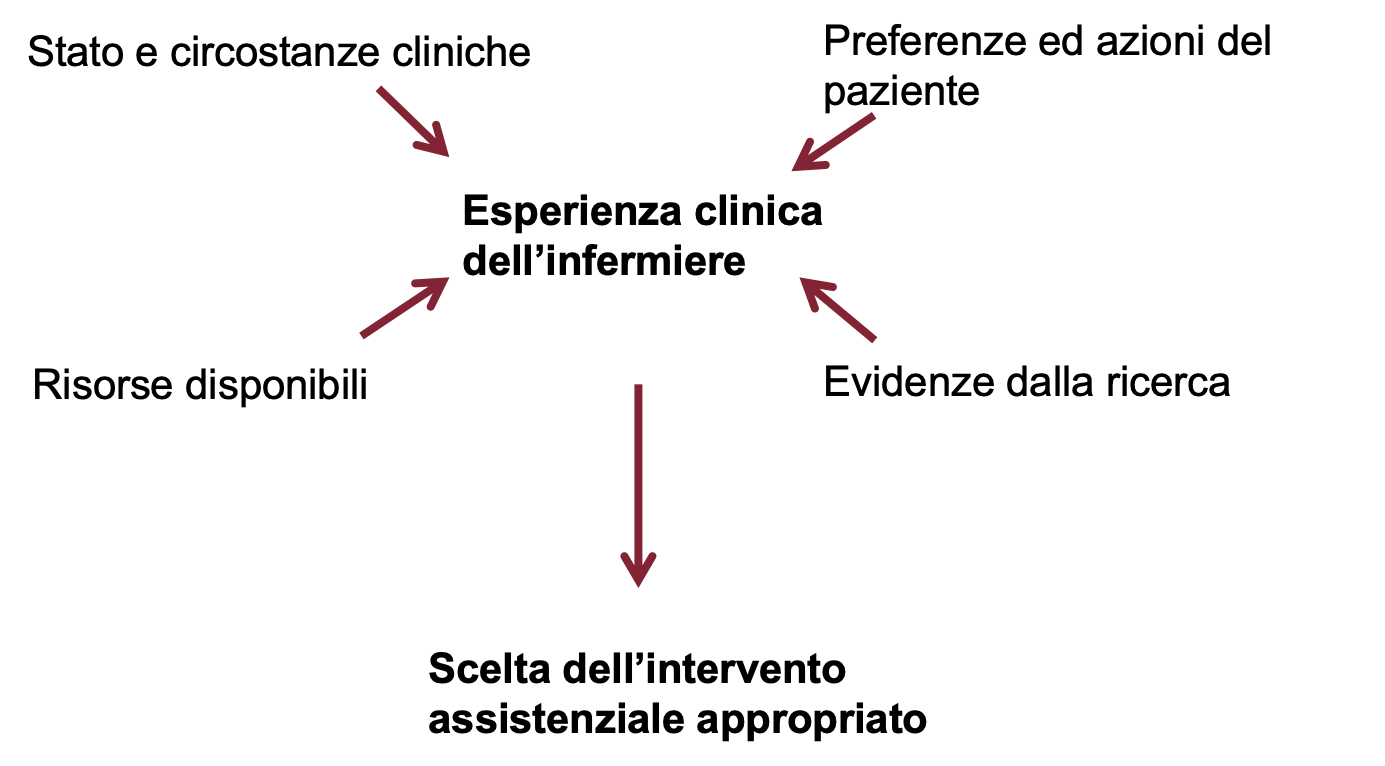
\includegraphics[width=0.8\textwidth,height=\textheight]{./img/mod-concettuale-ebn.png}

Gli elementi che vanno considerati sono:

\textbf{Stato e circostanze cliniche}. Lo stato e le circostanze cliniche (es. gravità della malattia, instabilità clinica, comorbidità) influenzano l'intensità assistenziale (o setting assistenziale). L'aspetto essenziale delle decisioni cliniche basate sull'evidenza è quello di effettuare azioni assistenziali appropriate alle specifiche circostanze del paziente.

\textbf{Preferenze ed azioni del paziente}. Le preferenze e le azioni del paziente si riferiscono alle aspettative che il paziente ha e che vanno considerate nella decisione clinica. Si noti come le azioni del paziente possono essere differenti dalle sue preferenze e/o desideri. Per esempio, un paziente può accettare ``a parole'' di perdere peso, smettere di fumare o prendere la terapia prescritta ma poi puo' non riuscire ``nei fatti'' a raggiugere questi obiettivi.

\textbf{Risorse disponibili}. Si riferiscono alle risorse utilizzabili per erogare l'assistenza infermieristica in un contesto organizzativo specifico in termini di dispositivi e presidi medici (qualità struttura), qualità del processo di assistenza, abilità e numerosità del personale, tempo a disposizione ecc.

\textbf{Evidenze dalla ricerca}. Nel nursing, come in tutte le scienze sanitarie, la migliore evidenza prodotta dalla ricerca si riferisce a studi epidemiologici che siano metodologicamente corretti e clinicamente rilevanti. Le linee guida e i protocolli diagnostico-terapeutici sono basati su prove (in inglese ``evidences'') di efficacia e sicurezza. Ne segue che le regole formali per interpretare i risultati della ricerca clinica devono essere insegnate come parte della regolare formazione infermieristica. Identificare le migliori evidenze scientifiche richiede rudimentali nozioni di epidemiologia.

\textbf{Esperienza personale}
L'esperienza clinica è il mezzo per integrare le quattro componenti sopra citate. Si riferisce all'abilità dell'infermiere di identificare i bisogni assistenziali del pz, prevedere i rischi durante la degenza /convalescenza, saper agire/affrontare gli interventi assistenziali più appropriati, saper comunicare le informazioni ai pazienti e ai loro familiari, saper fornire loro un ambiente che sia confortevole e di supporto al paziente.

\hypertarget{benefici-dellapproccio-evidence-based}{%
\subsection{Benefici dell'approccio ``evidence based''}\label{benefici-dellapproccio-evidence-based}}

Praticare EBN è da molti ritenuto necessario per erogare la migliore assistenza possibile e quindi rispettare l'obbligo degli infermieri verso la società. Le implicazioni del modello EBN sopra descritto sono che l'intuizione e l'esperienza clinica \emph{non sistematica} del professionista e la mera conoscenza delle tecniche non siano sufficienti a garantire standard assistenziali qualitativamente elevati.

Per esempio, Heater et al. (1988) hanno riassunto 84 studi condotti da infermieri che comprendevano 4.146 pazienti. I pazienti assistiti da professionisti che praticavano EBN avevano miglioramenti considerevoli in comportamenti, conoscenze, parametri fisiologici e psicosociali rispetto ai pazienti assistiti in maniera tradizionale.

Cui et al. (2018) hanno riassunto 9 studi condotti su \textgreater{}1000 infermieri. Gli infermieri che hanno studiato EBN hanno una maggiore attitudine al pensiero critico e all'applicazione dell'assistenza più appropriata.

Alcune conseguenze della non applicazione dei principi EBN sono la erogazione di prestazioni sanitarie non ottimali, l'esposizione dei pz a rischi non necessari, la determinazione di costi non giustificati, la difformità nella pratica infermieristica tra reparti ed ospedali oltre alla scarsa crescita professionale.

\hypertarget{ostacoli-e-limiti-allapplicazione-dellebn}{%
\subsection{Ostacoli e limiti all'applicazione dell'EBN}\label{ostacoli-e-limiti-allapplicazione-dellebn}}

Uno degli ostacoli allo sviluppo dell'EBN in Italia è rappresentato dalla resistenza del personale infermieristico al cambiamento: conservazione della tradizionale organizzazione per compiti e consuetudine alle routine. L'assenza di sufficiente razionalita' organizzativa e di adeguate motivazioni scientifiche a supporto delle attività̀ assistenziali determinano spreco di risorse professionali e bassa efficacia complessiva dell'assistenza. Questo si associa spesso a demotivazione e all'abbassamento dei livelli di professionalita' del personale infermieristico.

Un altro problema è costituito dall'assenza di risultati o risultati contrastanti della ricerca per alcuni quesiti clinici (``zone grigie'' della letteratura). In molti settori dell'assistenza, come più̀ in generale della medicina, vi sono numerose ed ampie zone grigie dove non sono reperibili evidenze sull'efficacia di un intervento assistenziale e/o delle sue alternative.

Altri ostacoli all'implementazione della EBN sono l'incremento continuo di nuove conoscenze che rende estremamente difficile per qualsiasi professionista mantenersi aggiornato e la scarsa trasferibilità dei risultati di alcune ricerche alla pratica clinica. Infine, la formazione universitaria fornisce solo in parte competenze specifiche per la ricerca e l'approccio critico alla letteratura sanitaria. A questo si sommano una scarsa conoscenza della lingua inglese, una limitata diffusione dei moderni strumenti d'informazione ed informatici nelle nostre strutture assistenziali.

\hypertarget{esercizio}{%
\section{Esercizio}\label{esercizio}}

\begin{enumerate}
\def\labelenumi{\arabic{enumi})}
\tightlist
\item
  Descrivi con parole tue le 5 componenti del modello EBN
\end{enumerate}

-- Stato e circostanze cliniche

-- Preferenze ed azioni del paziente

-- Risorse disponibili

-- Evidenze della ricerca

-- Esperienza personale

\begin{enumerate}
\def\labelenumi{\arabic{enumi})}
\setcounter{enumi}{1}
\item
  Quali sono le conseguenze di non seguire la pratica clinica basata sulle prove di efficacia?
\item
  Descrivi alcune dei limiti all'applicazione della EBN in Italia
\end{enumerate}

\hypertarget{le-fasi-della-infermieristica-basata-sulle-evidenze}{%
\section{Le fasi della infermieristica basata sulle evidenze}\label{le-fasi-della-infermieristica-basata-sulle-evidenze}}

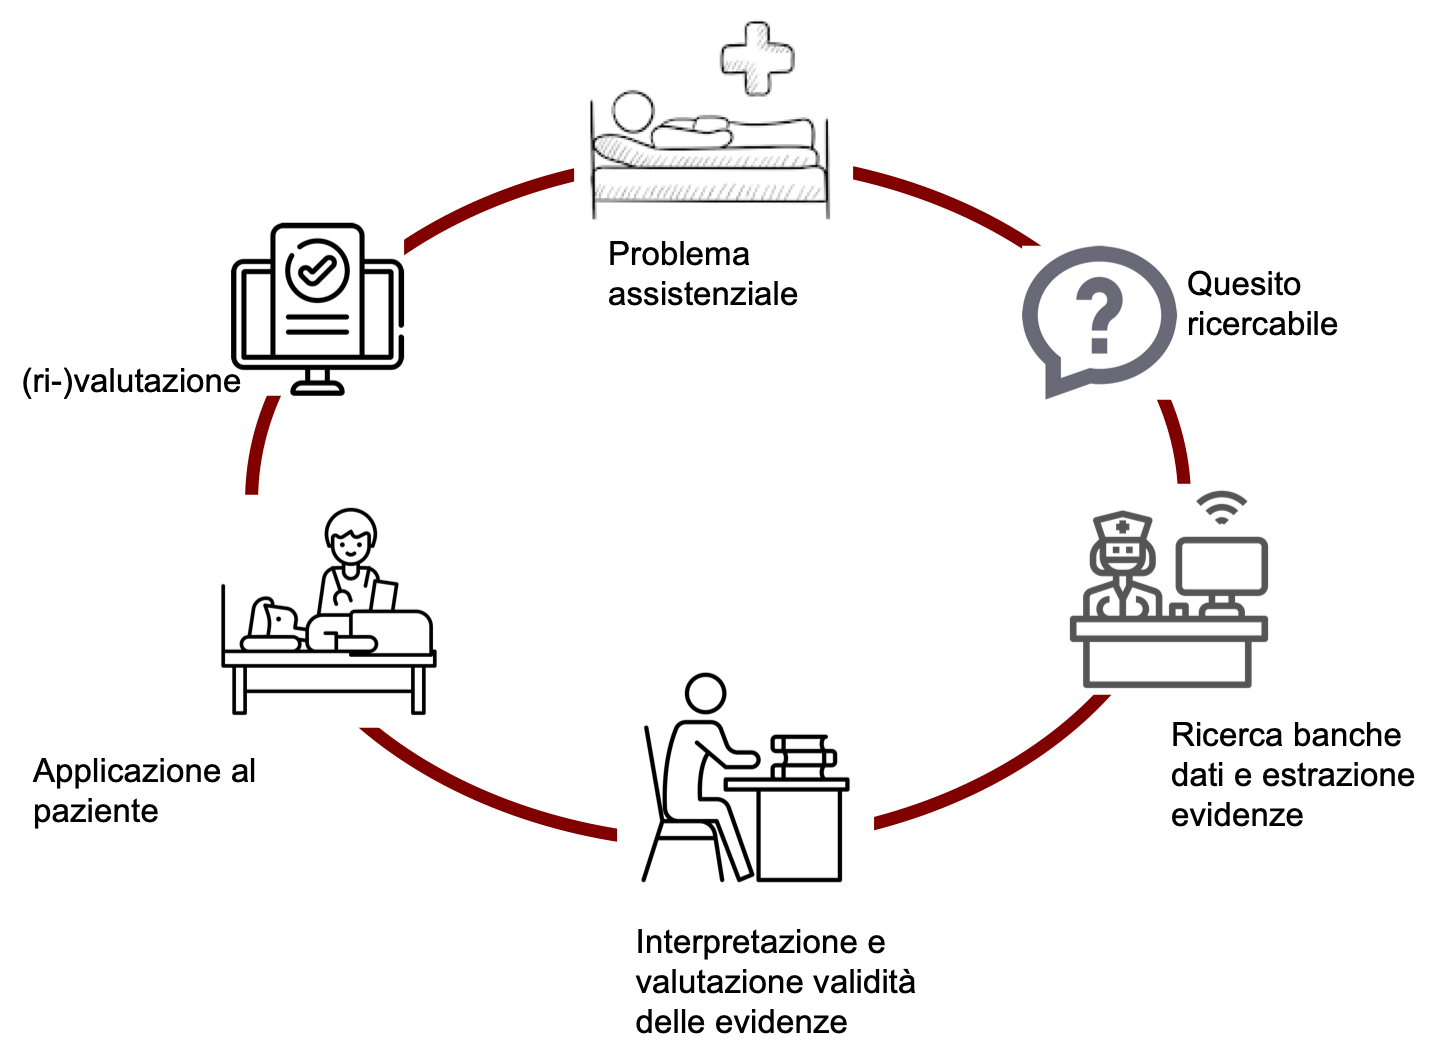
\includegraphics[width=0.8\textwidth,height=\textheight]{./img/ebn-ciclo.png}

Operativamente si possono identificare 5 fasi:

\begin{enumerate}
\def\labelenumi{\arabic{enumi})}
\item
  Identificare i problemi o i dubbi che derivano dalla pratica quotidiana o dall'assistenza ad un specifico paziente e tradurre queste incertezze in quesiti focalizzati e ricercabili (``quesito'' o ``dubbio'' assistenziale)
\item
  ricercare nella banche dati con apposite strategie gli studi epidemiologici pubblicati che, con disegni appropriati, aiutano a rispondere al quesito
\item
  interpretare ed analizzare criticamente gli studi raccolti
\item
  adeguare la pratica clinica alle indicazioni individuate
\item
  rivalutare periodicamente l'efficacia
\end{enumerate}

\textbf{Implicazioni}

Le implicazioni di questo modello di assistenza al paziente sono:

\begin{itemize}
\item
  l'infermiere e' proattivo nell'identificare i bisogni assistenziali dei pz che non sono soddisfatti efficacemente;
\item
  a partire dal bisogno del pz, e' in grado di formulare un quesito ricercabile nelle banche dati e condurre la ricerca (es. su PubMed);
\item
  l'infermiere conosce la struttura degli studi epidemiologici ed e' in grado di valutarli ed ottenere una risposta al quesito;
\item
  applica il risultato nell'assistenza al pz;
\item
  rivaluta periodicamente l'appropriatezza dell'intervento.
\end{itemize}

\hypertarget{problema-assistenziale-e-quesito-di-ricerca}{%
\section{Problema assistenziale e quesito di ricerca}\label{problema-assistenziale-e-quesito-di-ricerca}}

La prima fase del ciclo EBN riguarda l'individuazione del problema relativo all'assistenza e la sua trasformazione in un quesito di ricerca che possa essere utilizzato in una banca dati. Il problema assistenziale sono le domande che l'infermiere si pone ogni volta che visita un paziente e che individuano le informazioni di cui ha bisogno per prendere la migliore decisione in ambito assistenziale. Quindi tutto nasce dai bisogni/richieste assistenziali del paziente che rimangono ancora irrisolti e che possono essere inerenti la diagnosi, il trattamento (terapia), la prognosi, l'eziologia o la prevenzione di una certa condizione medica.

\textbf{Formulazione ed importanza del quesito di ricerca}
Il quesito di ricerca è fondamentale per il processo EBN. Esso deriva dal problema assistenziale che, a sua volta, origina dall'osservazione del paziente. ``Finché non si è in grado di formulare quesiti a cui è possibile rispondere, si è destinati a sprecare molto del limitato tempo dedicato alla ricerca ed alla consultazione della letteratura disponibile con la conseguenza di rimanere non solo frustrati, ma di vedere diminuire la propria competenza clinica'' (Chiari et al., 2011).

\textbf{Perchè è importante chiarire bene il quesito di ricerca?} Perchè dal quesito vengono estratte le parole chiave che useremo nella interrogazione della banca dati. Dalla chiara espressione del quesito di ricerca possiamo definire i criteri di inclusione o di esclusione, ovvero a quali pazienti possono essere applicati i risultati della ricerca. La tipologia del quesito indica anche quale tipo di studio dobbiamo cercare.

Un buon quesito di ricerca risulta solitamente costituito dalle seguenti componenti:

\begin{itemize}
\item
  Chiara definizione delle caratteristiche del soggetto da assistere (popolazione)
\item
  Tipo di azione che si intende attuare nei confronti del pz o fattore di rischio/prognostico di interesse (intervento)
\item
  Intervento o esposizione di confronto (confronto)
\item
  Risultati che si vogliono conseguire o eventi che si vogliono evitare (esito)
\end{itemize}

\begin{quote}
Per esempio: Come posso alleviare (questo particolare) dolore di (questo particolare) paziente in questa (particolare) fase della degenza?
Che tipo di comportamento preventivo devo consigliare a (questo particolare) paziente per evitare ricadute (in questa particolare fase della convalescenza) di questa (particolare) malattia?
Quale fattore di rischio a contribuito a causare la malattia di questo particolare paziente?
\end{quote}

\textbf{Quesiti di background} Riguardano gli aspetti generali di una patologia, intervento, situazione clinica, ecc. e riflettono la necessità di arricchimento/ aggiornamento culturale e di conoscenza generale.

\begin{quote}
Per esempio: quali tipi di complicanze possono manifestarsi nei portatori di cateteri vescicali? Quali tipi di medicazioni usare per i portatori di CVC? Cosa si può fare per ridurre il rischio di errori nella somministrazione di farmaci?
\end{quote}

\textbf{Quesiti di foreground (clinici)} I quesiti di foreground (o clinici) riguardano informazioni e conoscenze specifiche circa la gestione di un particolare paziente affetto da una determinata malattia o riguardano una specifica situazione.

\begin{quote}
Ad esempio: In un paziente con ictus è meglio posizionare i liquidi sull'arto plegico o su quello non plegico? Nel paziente anziano, quanto il rumore e la vibrazione determinata dal materasso antidecubito incide sul sonno e sul livello di stress? Nel paziente con ulcere cutanee infette, la terapia antibiotica sistemica è più efficace della terapia antibiotica topica?
\end{quote}

\hypertarget{il-metodo-pico}{%
\section{Il metodo PICO}\label{il-metodo-pico}}

Il ``dubbio'' assistenziale è di solito formulato in maniera discorsiva o narrativa e deve essere ``trasformato'' per poter diventare un quesito a cui è possibile dare una risposta. Il metodo \textbf{PICO} permette contestualizzare il quesito e di trasformare il quesito dalla forma narrattiva in una ``stringa'' di ricerca da inserire in una banca dati.

\textbf{P: Patient}. Descrivi il gruppo di pazienti o il problema clinico oggetto della ricerca. Come descriverei un gruppo di pazienti (popolazione) simile al mio? Considerare: eta', sesso, patologia, instabilita' clinica, stadiazione della malattia, storia personale e familiare, contesto socio-economico, storia di patologie pregresse ecc.

\textbf{I: Intervention}. Quale intervento sto prendendo in considerazione? Essere specifici. Puo' essere un trattamento o un intervento terapeutico sperimentale, nuova scala diagnostica, possesso di fattore eziologico/prognostico, una esposizione ad un fattore nocivo di origine ambientale ecc.

\textbf{C: Comparison}. Quale è l'alternativa da confrontare con l'intervento? Puo' essere nulla o piu' spesso un trattamento di controllo o un intervento standard, test diagnostico standard, assenza fattore eziologico/prognostico, la non esposizione ad un fattore nocivo di origine ambientale ecc.

\textbf{O: Outcome}. L'esito o risultato clinico a cui sono interessato. Quale effetto osservo in termini di esiti clinicamente rilevanti cone per es. la morte, guarigione, sopravvivenza, infezione, ecc.

\hypertarget{tipologia-quesito-domanda}{%
\subsection{Tipologia quesito / domanda}\label{tipologia-quesito-domanda}}

Una classificazione molto utile riguarda la tipologia del quesito di ricerca. I quesiti di ricerca possono riguardare il trattamento, l'eziologia, la prognosi o la diagnosi di una patologia.

I quesiti di \textbf{Trattamento (terapia)} riguardano domande sull' \emph{efficacia} degli interventi su pazienti affetti da uno o piu' patologie come per esempio valutazioni di efficacia di una terapia farmacologica o di una procedura assistenziale. Sono i quesiti piu' comuni nella pratica infermieristica.

I quesiti \textbf{Eziologici} riguardano domande sulle \emph{cause} dell'insorgenza di una condizione patologica. Di solito viene formulato un quesito eziologico quando si vogliono indagare i fattori di rischio di una certa patologia. Per esempio potremmo essere interessati a identificare le caratteristiche del paziente (come gli stili di vita, l'eta', le comorbidita' ecc.) piu' frequentemente associate con un alto rischio di infarto del miocardio. Sono spesso quesiti di interesse per l'infermiere che presta servizio presso i presidi territoriali (distretto).

I quesiti di \textbf{Prognosi} riguardano domande sull' \emph{evoluzione} di una patologia nei pz che ne sono gia' affetti. Si tenta quindi di identificare quei fattori (``fattori prognostici'') che sono associati con una migliore o peggiore prognosi. Per esempio potremmo essere interessati ad individuare i fattori (come l'eta', le comorbidita' ecc.) associate con un recupero funzionale piu' lento nei pazienti che hanno subito un infarto del miocardio. Sono quesiti comuni per l'infermiere ospedaliero.

I quesiti di \textbf{Diagnosi} riguardano domande sull'efficacia degli strumenti o di procedure diagnostiche. Per esempio domande concernenti l'accuratezza della valutazione iniziale o le diagnosi (identificazione dei problemi del paziente) ed il confronto tra diversi sistemi per ottenere una certa diagnosi infermieristica.

\begin{longtable}[]{@{}llr@{}}
\toprule
\begin{minipage}[b]{0.30\columnwidth}\raggedright
Tipo di quesito\strut
\end{minipage} & \begin{minipage}[b]{0.30\columnwidth}\raggedright
Significato\strut
\end{minipage} & \begin{minipage}[b]{0.30\columnwidth}\raggedleft
Esempio\strut
\end{minipage}\tabularnewline
\midrule
\endhead
\begin{minipage}[t]{0.30\columnwidth}\raggedright
Trattamento\strut
\end{minipage} & \begin{minipage}[t]{0.30\columnwidth}\raggedright
Efficacia di un intervento\strut
\end{minipage} & \begin{minipage}[t]{0.30\columnwidth}\raggedleft
E' il trattamento X piu' efficace del trattamento Y?\strut
\end{minipage}\tabularnewline
\begin{minipage}[t]{0.30\columnwidth}\raggedright
Eziologici\strut
\end{minipage} & \begin{minipage}[t]{0.30\columnwidth}\raggedright
Eziologia di una condizione\strut
\end{minipage} & \begin{minipage}[t]{0.30\columnwidth}\raggedleft
E' il diabete un fattore di rischio per l'infarto del miocardio?\strut
\end{minipage}\tabularnewline
\begin{minipage}[t]{0.30\columnwidth}\raggedright
Prognostici\strut
\end{minipage} & \begin{minipage}[t]{0.30\columnwidth}\raggedright
Evoluzione di una condizione\strut
\end{minipage} & \begin{minipage}[t]{0.30\columnwidth}\raggedleft
Nel paziente ricoverato per infarto del miocardio, e' il diabete collegato con una degenza piu' lunga?\strut
\end{minipage}\tabularnewline
\begin{minipage}[t]{0.30\columnwidth}\raggedright
Diagnosi\strut
\end{minipage} & \begin{minipage}[t]{0.30\columnwidth}\raggedright
Accuratezza diagnostica\strut
\end{minipage} & \begin{minipage}[t]{0.30\columnwidth}\raggedleft
E' una certa diagnosi infermieristica accurata?\strut
\end{minipage}\tabularnewline
\bottomrule
\end{longtable}

\hypertarget{esempi}{%
\subsection{Esempi}\label{esempi}}

\textbf{Quesito di trattamento}

Siete in servizio presso il reparto di pediatria. Un collega vi chiede se un bambino di 8 anni che deve essere sottoposto a sutura di una ferita lacero-contusa, l'applicazione di pomata anestetica sia meno dolorosa della somministrazione di lidocaina sottocutanea per l'analgesia (livello di dolore percepito).

-- Paziente: Pediatrico con ferita lacero-contusa

-- Intervento: Trattamento con pomata anestetica

-- Confronto: Trattamento con lidocaina sottocutanea

-- Outcome: livello dolore percepito

\textbf{Quesito eziologico}

Sei un coordinatore di un reparto di medicina generale. Un pz di 50 anni ex fumatore e sovrapeso ricoverato per infarto miocardio vi chiede se praticare uno sport come la corsa a livello amatoriale possa essere stata la causa della sua malattia.Prima di rispondere decidi di svolgere la ricerca nelle banche dati.

-- Paziente: individuo ex-fumatore, sovrapeso

-- Intervento: Pratica sport aerobico

-- Confronto: Non pratica sport

-- Outcome: infarto

\textbf{Quesito prognostico}

Sei un coordinatore di un reparto di medicina generale. Un pz di 50 anni ex fumatore e sovrapeso ricoverato per infarto miocardio vi chiede se praticare uno sport come la corsa a livello amatoriale possa provocare un recidive/ricadute della sua malattia. Prima di rispondere decidi di svolgere la ricerca nelle banche dati.

-- Paziente: pz exfumatore, sovrapeso, infartuato

-- Intervento: Pratica sport aerobico

-- Confronto: Non pratica sport

-- Outcome: recidive

\textbf{Quesito diagnostico}

Un coordinatore di un reparto di geriatria e ti chiedono un consiglio relativamente alla migliore scala per diagnosticare il rischio di caduta nei pz affetti da demenza grave che entrano in reparto. Individui due scale: la scala di Conley e la scala Stratify. Ti chiedi quale sia la piu' accurata per pz di questo tipo.

-- Paziente: pz geriatrico con demenza grave

-- Intervento: Scala Conley

-- Confronto: Scala Stratify

-- Outcome: cadute in reparto

\hypertarget{ricerca-delle-evidenze}{%
\section{Ricerca delle evidenze}\label{ricerca-delle-evidenze}}

La ricerca delle evidenze e' il secondo step nel ciclo EBN. Per prima cosa chiariamo cosa sono le ``evidenze'' e dove le possiamo reperire in maniera efficiente e poi facciamo un esempio di interrogazione della banca dati PubMed.

\textbf{Evidenze = prove scientifiche}. Come detto, le ``prove di efficacia'' sono delle dimostrazioni scientifiche che una determinata azione assistenziale (trattamento, diagnosi ecc.) funziona per lo scopo per la quale la facciamo. In altri termini sono i risultati di ricerche di buona qualita' che sono state pubblicati su riviste specializzate dopo essere stati sottoposti al processo di revisione tra pari (peer review). Ovvero sottoposte alla verifica preventiva della ricerca di professionisti/esperti del settore specifico. Una volta pubblicato, le conclusioni e le metodologie di un lavoro possono essere verificate da altri ricercatori su altri pazienti.

\textbf{Cosa viene archiviato in forma ricercabile?} Tutti gli abstract delle ricerche pubblicate su riviste internazionali vengono indicizzate nelle banche banche dati. Gli abstract riflettono la struttura dell'intero articolo scientifico che di solito e' composto dalle seguenti sezioni:

-- Introduction = motivazioni per affrontare quel particolare quesito di ricerca

-- Methods = Come è stata svolta la ricerca e in che modo hanno analizzato i risultati

-- Results = Cosa è stato provato/scoperto

-- Discussion = Cosa gli autori pensano possano significare i risultati ottenuti

-- Conclusions = Quali sono le implicazioni, il significato per l'assistenza infermieristica

\textbf{Quale studio è utile per EBN?} Al giorno d'oggi c'è sovracarico di informazione disponibile: esistono \textgreater{}50 milioni di pubblicazioni biomediche disponibili in database, viene aggiunta una pubblicazione ogni 30 secondi. Per es. con una ricerca su PubMed su un problema clinico comune si ottengono facilmente migliaglia di titoli ed abstract di pubblicazioni tra le quali e' difficile orientarsi. Tuttavia, le informazioni contenute nel 70 - 80\% di questi articoli sono spesso inutili perchè derivanti da studi costruiti con metodologie scorrette o perchè irrilevanti dal punto di vista clinico o perchè obsoleti.

Perchè sia rilevante per EBN uno studio deve:

\begin{enumerate}
\def\labelenumi{\arabic{enumi})}
\item
  Essere rilevante: dare indicazioni utili per la propria pratica clinica. Quindi deve dare un informazione orientata al paziente ovvero riguardare esiti clinicamente significativi (eventi maggiori, mortalità, qualità di vita).
\item
  Essere valido: devono essere verificate la validità interna (assenza di errori casuali e sistematici) e la validità esterna (trasferibilita' dei risultati ad altri contesti assistenziali)
\item
  L'informazione deve essere reperibile in maniera efficiente in termini di tempo, costi, energie mentali
\end{enumerate}

\hypertarget{ricerca-nelle-banche-dati}{%
\section{Ricerca nelle banche dati}\label{ricerca-nelle-banche-dati}}

L'infomazione relativa alle ricerche pubblicate (e a volte ancora non pubblicate, cioè in forma di pre-prints) può essere ricercata con i comuni motori di ricerca o nelle apposite banche dati biomediche.

\textbf{Motori di ricerca (google)}. I contenuti di una ricerca che vengono restituiti da google non devono adeguarsi ad alcuno standard qualitativo e l'informazione non è organizzata o stabile (cioe' puo' scomparire). I risultati di una ricerca su google e' una lista di link a pagine web e sono il prodotto di algoritmi automatici non controllati dall'utente. Non consentono ricerche complesse o combinate e hanno poche possibilita' di applicare limiti e/o filtri. Tuttavia sono semplici da utilizzare e consentono di recuperare tutte le informazioni non indicizzate nelle banche dati (come per es. la letteratura grigia come i rapporti tecnici).

\textbf{Banche dati}. Le banche dati come per es. Pubmed, Scopus, Chinal sono dei cataloghi che contengono i riferimenti bibliografici di ogni ricerca pubblicata.I contenuti sono indicizzati da specialisti del settore e, come detto, sono stati precedentemente sottoposti a peer review. L'informazione contenuta è organizzata e stabile nel tempo, consentono la ricerca per parole chiave in molteplici campi (per es. nel titolo, nell'abstract, negli autori ecc.), consentono di visualizzare la cronologia delle ricerche effettuate, di combinare le ricerche tra loro, di salvare le ricerche, di impostare degli avvisi sulle novità concernenti le ricerche effettuate ed e' possibile raffinare la ricerca tramite filtri e limiti dettagliati e peculiari.

\textbf{Cosa devo valutare?} Dalla lettura dell'abstract in genere si capisce se l'articolo e' rilevante per rispondere ad un determinato quesito di ricerca. Se riteniamo, dopo la lettura dell'abstract, che un articolo sia rilevante passeremo al reperimento e successiva valutazione critica dei risultati previa lettura dell'intera pubblicazione. Come vedremo nei capitolo seguenti, la valutazione critica di una ricerca prevede l'analisi dei metodi e dei risultati, ovvero le sezioni Methods e Results dell'articolo.

\hypertarget{pubmed}{%
\subsection{PubMed}\label{pubmed}}

La banca dati PubMed {[}(\url{https://www.ncbi.nlm.nih.gov/pubmed/}){]} è la più utilizzata in campo biomedico. Una volta definito il quesito di ricerca in formato PICO, posso inserire le varie parole chiave, combinarle con opportuni \emph{operatori booleani} e cercarle nei campi indicizzati (es. tutto l'abstract, il titolo\ldots{}) degli abstract che sono stati archiviati nella banca dati.

\textbf{Operatori booleani} si tratta di operatori logici che possono essere utilizzati per stabilire una particolare relazione tra i termini da ricercare; quelli utilizzabili in PubMed sono i tre più noti: \texttt{AND}, \texttt{OR}, \texttt{NOT}, da scriversi in maiuscolo tra i due termini posti in relazione.

-- \texttt{AND} recupera documenti che contengono entrambi i termini;

-- \texttt{OR} recupera documenti che contengono almeno uno dei due termini, oppure entrambi;

-- \texttt{NOT} recupera documenti che contengono solo il primo dei due termini, escludendo il secondo o i documenti in cui ci sia compresenza dei due.

\textbf{Esempi:}

-- \texttt{Pressure\ ulcers\ AND\ geriatric}: i documenti contengono contemporaneamente i termini \texttt{Pressure\ ulcers} e \texttt{geriatric}

-- \texttt{Pressure\ ulcers\ OR\ geriatric}: i documenti contengono o \texttt{Pressure\ ulcers} o \texttt{geriatric}, oppure entrambi;

-- \texttt{Pressure\ ulcers\ NOT\ geriatric}: i documenti contengono solo \texttt{Pressure\ ulcers}, escludendo quelli in cui è presente anche \texttt{geriatric}.

La ricerca in cui i termini sono combinati con l'operatore \texttt{OR} produce un maggior numero di risultati rispetto alla stessa ricerca impostata con \texttt{NOT}. L'operatore \texttt{AND}, invece, restringe ulteriormente la ricerca.

\textbf{Uso di parentesi}. Nelle ricerche più articolate, in cui vengono combinati diversi termini, è possibile utilizzare le parentesi per stabilire un ordine di priorità nella lettura della stringa di ricerca: in assenza di parentesi, infatti, il sistema legge sequenzialmente, da sinistra a destra. Le parentesi \texttt{(\ )} indicano l'ordine con cui i termini vengono ricercati: quelli tra parentesi sono analizzati per primi. Importanti per estrarre i termini secondo l'eventuale condizione booleana. Es. volete ricercare come assistere un pz con infezioni specifiche delle piaghe da decubito, una stringa con \texttt{nursing\ AND\ bedsores\ OR\ infections} avra' come esito: \texttt{nursing\ AND\ bedsores\ +\ infections}. Per avere il risultato voluto \texttt{nursing\ AND\ bedsores\ +\ nursing\ AND\ infections} si possono utilizzare le parentesi in questo modo: \texttt{nursing\ AND\ (bedsores\ OR\ infections)}

\textbf{Caratteri jolly}. Le \texttt{“\ ”} (virgolette) permettono di ricercare due o più termini nell'ordine preciso con il quale vengono scritte. Es: \texttt{“pressure\ ulcers”} Il motore cerchera' nei vari campi testuali esattamente le due parole e nel preciso ordine in cui sono state scritte. Se non fossero presenti le virgolette l'ordine non sarebbe considerato, sarebbe calcolata la sola presenza delle 2 parole nel testo (\texttt{pressure\ OR\ ulcers}).

L'asterisco \texttt{*} Permette di ricercare all'interno dei campi tutte le parole con una stessa radice. Es. \texttt{ulcer*} Il motore cerchera' nei vari campi testuali tutte quelle parole che cominciano con ulcer come ulcer, ulcers, ulceration\ldots{}

\textbf{Uso dei termini MeSH}. Nel menu a tendina e' possibile selezionare l'archivio ``MeSH''. Si tratta di un ``dizionario dei sinonimi'' molto utile. Per es. selezionando il termine MeSH \texttt{“pressure\ ulcers”}, comprendiamo nella ricerca tutti gli altri sinonimi di ulcere da pressione (Bedsores, Decubitus Ulcers) senza che li dobbiamo inserire manualmente nei campi di ricerca.

\textbf{Limiti}. Sulla homepage di PubMed, nel menu sulla sinistra, è possibile utilizzare lo strumento \texttt{"Limits"} per delimitare la ricerca. Diversi menu a tendina e box selezionabili permettono di aggiungere termini in uno specifico campo (autori, titoli di periodici) e di scegliere varie opzioni di restituizone dei records come i soli record provvisti di abstract e/o di full-text, la data di pubblicazione degli articoli, il tipo di pubblicazione, il tipo di studio e moltio altri (si veda additional filters).

\textbf{Salvataggio delle ricerche effettuate}. Attraverso il menu a tendina ``send to'', inoltre, sono possibili diverse azioni: visualizzare i risultati in formato testo (text), salvare su file nel formato scelto (file); stampare in formato testo (selezionando il numero di voci per pagina desiderato); inviare il risultato della ricerca alla propria e-mail o usufruire di altri servizi di archiviazione o elaborazione dei dati.

\hypertarget{esempio}{%
\subsection{Esempio}\label{esempio}}

Siete interessati a sapere di piu' sull'efficacia della movimentazione (\texttt{repositioning}) sulla prevenzione delle ulcere da pressione (\texttt{pressure\ ulcer}) nel paziente geriatrico (\texttt{geriatric}). Preferibilmente ci indirizzeremo ad una revisione sistematica o ad una meta-analisi.

Di seguito una possibile strategia della ricerca, con il numero di records restituiti ( \emph{ricerca effettuata il 29-01-2021}):

\begin{longtable}[]{@{}lr@{}}
\toprule
Termini & Records\tabularnewline
\midrule
\endhead
\texttt{pressure\ ulcers} & 20313\tabularnewline
\texttt{pressure\ ulcers\ {[}MeSH{]}\ AND\ geriatric} & 707\tabularnewline
\texttt{pressure\ ulcers\ {[}MeSH{]}\ AND\ geriatric\ AND\ repositioning} & 23\tabularnewline
\bottomrule
\end{longtable}

Poi selezioniamo i box dei \texttt{limits\ to\ Systematic\ review} e quello delle \texttt{meta-analysis}. La banca dati ci restituisce 5 articoli di cui due abbastanza recenti che, a giudicare dalla lettura dell'abstract, potrebbero rispondere al nostro quesito di ricerca. Questi ( \emph{ricerca effettuata il 29-01-2021}) sono:

Lozano-Montoya I, Vélez-Díaz-Pallarés M, Abraha I, Cherubini A, Soiza RL, O'Mahony D, Montero-Errasquín B, Correa-Pérez A, Cruz-Jentoft AJ. Nonpharmacologic Interventions to Prevent Pressure Ulcers in Older Patients: An Overview of Systematic Reviews (The Software ENgine for the Assessment and optimization of drug and non-drug Therapy in Older peRsons {[}SENATOR{]} Definition of Optimal Evidence-Based Non-drug Therapies in Older People {[}ONTOP{]} Series). J Am Med Dir Assoc. 2016 Apr 1;17(4):370.e1-10. doi: 10.1016/j.jamda.2015.12.091. Epub 2016 Feb 5. PMID: 26857298.

Vélez-Díaz-Pallarés M, Lozano-Montoya I, Abraha I, Cherubini A, Soiza RL, O'Mahony D, Montero-Errasquín B, Cruz-Jentoft AJ. Nonpharmacologic Interventions to Heal Pressure Ulcers in Older Patients: An Overview of Systematic Reviews (The SENATOR-ONTOP Series). J Am Med Dir Assoc. 2015 Jun 1;16(6):448-69. doi: 10.1016/j.jamda.2015.01.083. Epub 2015 Feb 27. PMID: 25737261.

Reddy M. Pressure ulcers. BMJ Clin Evid. 2011 Apr 28;2011:1901. PMID: 21524319; PMCID: PMC3217823.

Reddy M, Gill SS, Rochon PA. Preventing pressure ulcers: a systematic review. JAMA. 2006 Aug 23;296(8):974-84. doi: 10.1001/jama.296.8.974. PMID: 16926357.

\hypertarget{esercizi}{%
\subsection{Esercizi}\label{esercizi}}

Lavorate come infermiere nel reparto di pediatria (child). Vi chiedete se lo iodopovidone (povidone iodine) sia piu' efficace della clorexidina (chlorhexidine) nel prevenire le infezioni del sito chirurgico (surgical site infections).
Prima definite il PICO e poi in Pubmed (\url{https://www.ncbi.nlm.nih.gov/pubmed/}) effettuare la ricerca usando opportunamente l'operatori booleano (AND, OR, NOT), le parentesi, virgolette e l'asterisco se necessari.

\hypertarget{che-cosa-uxe8-lepidemiologia}{%
\section{Che cosa è l'epidemiologia}\label{che-cosa-uxe8-lepidemiologia}}

L'infermiere ha tra i sui obiettivi quello di offrire la migliore assistenza possibile per i pazienti. Abbiamo visto che le pratiche infermieristiche vengono continuamente aggiornate tramite i risultati della ricerca scientifica. Infatti, la ricerca è il ``tentativo di incrementare le conoscenze disponibili, mediante la scoperta di nuovi fatti o relazioni attraverso un'indagine sistematica'' e si basa sul metodo scientifico.

La ricerca clinica è l'oggetto dell'epidemiologia. Per questo motivo l'infermiere che vuole praticare EBN deve essere in grado di interpretare criticamente i risultati degli studi epidemiologici e conoscerne a grandi linee la struttura, le diverse tipologie e sapere individuare gli eventuali punti di forza e principali limiti.
\{figura ricerca met scientifico\}

\hypertarget{definizioni}{%
\subsection{Definizioni}\label{definizioni}}

L'epidemiologia fornisce ai professionisti della sanità l'insieme dei metodi che permettono di effettuare ricerca in ambito clinico, leggere criticamente la letteratura scientifica ed interpretarne i risultati. È una disciplina metodologica che studia

\begin{quote}
la distribuzione e la frequenza degli esiti di salute e dei loro determinanti nelle popolazioni e l'applicazione dei risultati/conoscenza prodotta in sanità pubblica
\end{quote}

Esaminiamo brevemente le componenti della definizione che abbiamo proposto:

\textbf{Esito (outcome)} L'epidemiologia studia sia gli esiti ``negativi'' sia gli esiti ``positivi'' per la salute (in inglese: esito = \emph{outcome}). Sono esempi di esiti clinici negativi per la salute: morte, ricadute, complicanze, ulcere da pressione, difficoltà (sibilo) respiratoria ecc.). Esempi di esiti positivi: guarigione, qualità vita, assenza di ricadute\ldots{}(cute integra, remissione sintomi respiratori, diminuzione dolore\ldots{})

\textbf{Determinanti} Rappresenta lo specifico intervento assistenziale di cui si vuole testare l'efficacia o più in generale tutti quei fattori che sono, almeno in teoria, associati con l'esito. Quindi può essere un trattamento (es. applicazione di lidocaina) oppure il possesso di un fattore di rischio (per es. essere obeso). In altre parole sono i fattori che sono associati con un maggiore / minore rischio di esito.

\textbf{Popolazione} La procedura assistenziale appropriata per il singolo paziente viene individuata partendo da osservazioni condotte su gruppi di pazienti con caratteristiche simili.

La popolazione può essere costituita da pz in regime di degenza (si parla quindi di ``popolazione ospedalizzata'') che hanno le stesse caratteristiche di presentazione del decorso della malattia, le stesse comorbidità, uguale trattamento terapeutico, appartengono allo stesso reparto ecc.

Se l'intervento infermieristico è di tipo preventivo, l'idonea strategia viene individuata su osservazioni condotte su individui non ospedalizzati, ovvero nel loro ambiente di vita e di lavoro (``popolazione generale''), con le loro caratteristiche socio-demografiche, stili ed ambienti di vita, dal possesso o meno di fattori di rischio ecc.

\hypertarget{tipi-principali-di-studi-epidemiologici}{%
\subsection{Tipi principali di studi epidemiologici}\label{tipi-principali-di-studi-epidemiologici}}

Come abbiamo visto in precedenza i quesiti di ricerca possono riguardare diversi aspetti dell'assistenza infermieristica (trattamento, eziologia, prognosi e diagnosi). Anche i principali studi epidemiologici hanno una struttura diversa a seconda degli obiettivi specifici della ricerca.

Alcuni degli obiettivi degli studi epidemiologici sono:

-- Descrizione dei bisogni di salute;

-- Descrizione dei bisogni assistenziali;

-- Individuazione di fattori di rischio per la salute in popolazioni target (per es. obesità infantile);

-- Individuazione di fattori prognostici per il decorso clinico in popolazioni di pz

-- Valutazione di efficacia degli interventi clinici;

-- Valutazione di efficacia di interventi disposti sulla popolazione (per es. vaccinazione)

Come vedremo nel proseguo del corso, gli studi epidemiologici principali per l'EBN sono gli studi sperimentali (o studi di trattamento), gli studi di corte, gli studi caso controllo e gli studi trasversali. Una categoria di studi secondari molto importante e' rappresentata dalle revisioni sitematiche e meta-analisi che integrano i risultati di piu' studi primari offrendo all'infermiere una sintesi delle evidenze relative ad un determinato quesito di ricerca.

Gli studi sperimentali hanno l'obiettivo di verificare l'efficacia di trattamenti preventivi o terapeutici. Comprendono i trial clinici, che sono descritti nel capitolo 3. Gli studi di corte, caso-controllo e gli studi trasversali sono studi osservazionali e hanno l'obiettivo di verificare l'effetto delle esposizioni (eziologia) o possesso di un fattore prognostico sugli outcome di salute. Sono descritti nel capitolo 4. Le revisioni sistematiche e meta-analisi sono analisi di piu' studi primari (sperimentali o osservazionali) e saranno l'oggetto del capitolo 5. Menzioniamo inoltre anche degli studi puramente descrittivi, i case report, che sono utilizzati nelle scienze mediche per descrivere il decorso clinico o la presentazione sinomatologica inusuale di determinati pazienti. Più case reports simili formano una case series (serie di casi).

Come vedremo nei capitoli successivi, i quattro modelli di studio che abbiamo menzionato si adattano con diversa efficicacia ai diversi quesiti assistenziali. Gli studi sperimentali sono particolarmente adatti in caso di quesiti di trattamento (es. efficacia terapia / intervento preventivo), gli studi di corte e quelli caso controllo ai quesiti prognostici e a quelli eziologici, gli studi trasversali ai quesiti diagnostici.

\hypertarget{fonti-di-conoscenza}{%
\subsection{Fonti di conoscenza}\label{fonti-di-conoscenza}}

Le fonti di conoscenza in EBN possono essere di tipo primario, secondario o terziario.

Gli \textbf{studi primari} descrivono le singole ricerche e si basano su (tanti) dati individuali (dei singoli pazienti). Sono le fonti di conoscenza sulle quali e' piu' facile verificare la validita' interna. Come detto in precedenza, i 4 modelli principali di studi epidemiologici (studio sperimentale, di corte, caso-controllo e trasversale) vengono scelti dai ricercatori in base alla tipologia di quesito e ad altre considerazioni di fattibilità dello studio.
Pubblicazioni secondarie.

Gli \textbf{studi secondari} o integrativi hanno lo scopo di riassumere e trarre le conclusioni dagli studi primari. Esempio: review sistematiche, metanalisi, linee guida. Sono le fonti di conoscenza migliori per verificare la generalita' dei risultati riportati nelle fonti primarie. Quindi esistono meta-analisi di studi sprimentali, studi di corte ecc.

Infine le \textbf{fonti terziarie} sono quelle tradizionali come il parere di un collega esperto, libri, riviste, revisioni narrative.

\hypertarget{piramide-delle-evidenze}{%
\subsection{Piramide delle evidenze}\label{piramide-delle-evidenze}}

I diversi tipi di studi epidemiologici hanno diverse caratteristiche di validità interna. Alcuni sono più soggetti a errori sistematici di altri e quindi devono essere valutati criticamente prima di applicare il risultato nella pratica clinica. La cosidetta \textbf{piramide delle evidenze} esprime una gerarchia delle prove di efficacia in base al tipo di studio o in base alla sorgente di conoscenza. Ovviamente questa e' una semplificazione. Per es. uno studio di corte ben condotto produce evidenze migliori rispetto ad un trial clinico con problemi di validita' interna e/o esterna. Per questo motivo, l'attuale sistema di valutazione della qualita' delle evidenze si basa su un metodo piu' complesso (il metodo GRADE), per il quale si rimanda ai riferimenti riportati in bibliografia.

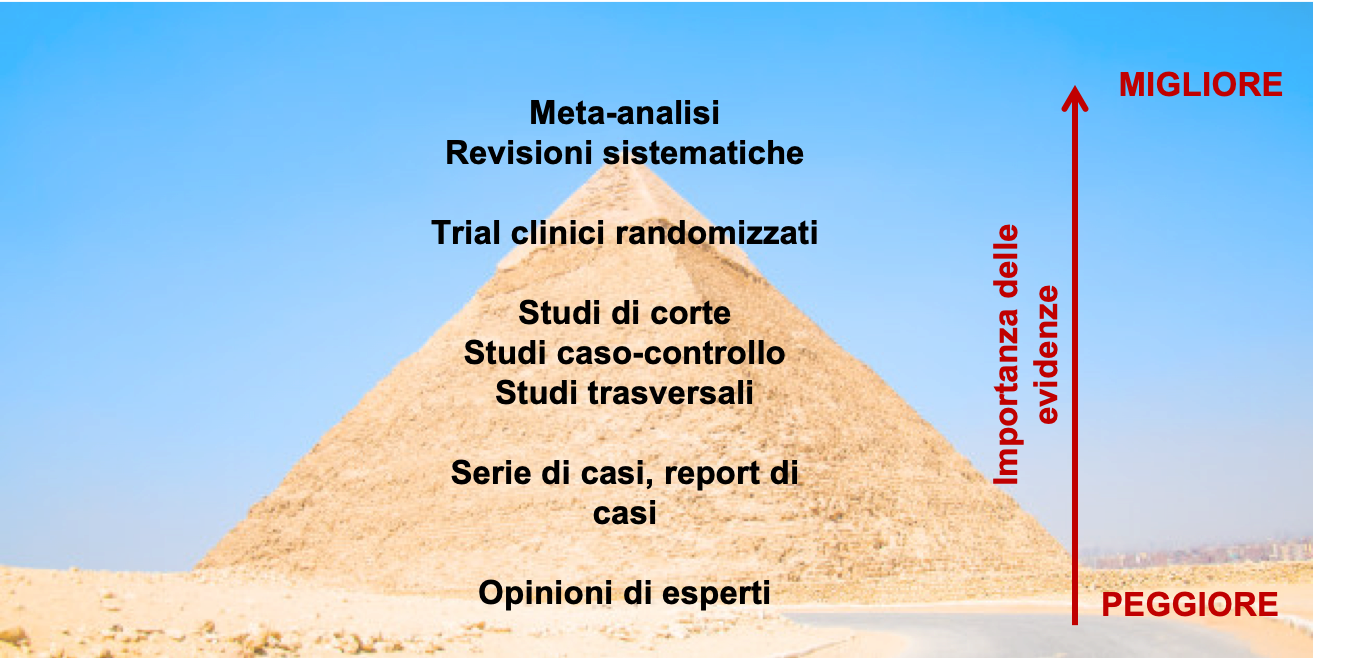
\includegraphics[width=0.8\textwidth,height=\textheight]{./img/piramide.png}


\hypertarget{esercizio-1}{%
\subsection{Esercizio}\label{esercizio-1}}

Per ogni quesito di ricerca individua quale è la popolazione, l'esito ed il determinante studiato.

\begin{enumerate}
\def\labelenumi{\arabic{enumi}.}
\tightlist
\item
  Esempio: La mobilizzazione precoce diminuisce il rischio di ulcere da pressione nei pz allettati per frattura all'anca ? Risposta:
\end{enumerate}

-- Popolazione: Pz allettati per frattura anca

-- Esito: lesioni da pressione

-- Determinante dell'esito: mobilizzazione precoce

\begin{enumerate}
\def\labelenumi{\arabic{enumi}.}
\setcounter{enumi}{1}
\item
  L'esposizione a fumo passivo determina sintomi respiratori nei bambini \textless{} 6 anni?
\item
  L'obesità negli adulti \textgreater{}55 anni aumenta il rischio di infarto?
\item
  L'incontinenza nell'anziano ricoverato aumenta il rischio di cadute accidentali in reparto?
\item
  Il riposizionamento del pz ogni 4h diminuisce il rischio di lesioni da pressione del pz immobilizzato per frattura agli arti?
\item
  La terapia con eparina diminuisce il rischio di trombosi venosa profonda nel paziente anziano ricoverato per polmonite interstiziale?
\end{enumerate}

\hypertarget{letture-e-risorse-utili}{%
\section{Letture e risorse utili}\label{letture-e-risorse-utili}}

\href{https://bal.lazio.it/wp-content/uploads/2017/05/Il-metodo-GRADE.pdf}{Il metodo GRADE -- Laura Amato, Luca De Fiore, Elena Parmelli, Marina Davoli}

\hypertarget{studi-di-trattamento}{%
\chapter{Studi di trattamento}\label{studi-di-trattamento}}

L'obiettivo degli studi di trattamento e' verificare l'efficacia di un intervento rispetto allo standard di riferimento. In questi studi si interviene assegnando gli individui che partecipano allo studio a due o più gruppi che si differenziano per il ricevere o meno il trattamento ``sperimentale''. L'intervento puo' essere preventivo o terapeutico. Sono detti anche studi di intervento o studi sperimentali o trial.
L'attiva manipolazione dell'assegnazione (o meno) del trattamento «sperimentale», ovvero dello status di esposizione, con \emph{lo scopo esplicito di verificarne la sua efficacia} è la caratteristica che distingue gli studi sperimentali (in inglese «trial») dagli studi osservazionali. Spesso (ma non sempre) lo scopo esplicito dello studio e' verificare se il trattamento sperimentale e' piu' efficace del trattamento standard.

E' opportuno far notare che anche in molti studi clinici osservazionali vengono confrontati, di solito retrospettivamente, gruppi di pazienti che ricevono uno o piu' trattamenti diversi. Tuttavia, negli studi osservazionali lo sperimentare non interviene nel processo di assegnazione dei pz ai diversi trattamenti che viene invece deciso secondo la routine clinica.
Molte persone sono implicate in uno studio sperimentale, ognuno con la sua professionalita' ed i suoi compiti specifici.

\hypertarget{tipologie}{%
\section{Tipologie}\label{tipologie}}

Vi sono diversi modi di classificare gli studi sperimentali.

Nei \textbf{trial individuali} le unita' campionarie che vengono assegnate ai gruppi a confronto (sperimentale vs controllo) sono i singoli pazienti mentre nei \textbf{trial di comunità} le unita' campionare sono gruppi di individui (comunità), come per es. reparti ospedalieri. I \textbf{trial preventivi} studiano gli interventi che evitano l'insorgenza della patologia, sono condotti su individui sani, spesso in gruppi a alto rischio, e possono riguardare l'esposizione ad un potenziale fattore benefico (es. vitamine, farmaci anticolesterolo) oppure interventi educativi che portano a migliori stili di vita (cambiamento dieta, esercizio fisico, uso del profilattico). La maggior parte degli studi sperimentali riguardano la valutazione di interventi clinici terapeutici (\textbf{trial terapeutici}) in ambiente clinico (\textbf{trial clinici}). Un ipotetico studio sperimentale che voglia verificare l'efficacia di un intervento educativo nelle scuole per la prevenzione delle malattie sessualmente trasmesse quindi e' un trial preventivo di comunita'.

Nei \textbf{trial controllati} e' presente un gruppo che riceve il trattamento di controllo che e' invece assente nei \textbf{trial non controllati}. Questi ultimi possono per esempio riguardare la sperimentazione di farmaci in fase 1 (tollerabilita' su volontari) e fase 2 (determinazione della dose-risposta su volontari malati). I \textbf{trial clinici randomizzati (RCT)} sono i trial piu' frequentemente utilizzati per la determinazione dell'efficacia di un trattamento. Questi sono spesso condotti in ambito clinico, sono randomizzati e con presenza di un gruppo di controllo. L'acronimo inglese RCT sta per randomized controlled trial. Nei \textbf{trial non randomizzati} l'assegnazione ai due gruppi in studio non e' casuale e puo' essere effettuata per es. secondo l'ordine di arrivo in reparto.

Nei \textbf{trial di superiorita'} si verifica se il trattamento sperimentale e' superiore (piu' afficace) al trattamento di confronto mentre nei \textbf{trial di equivalenza} e in quelli di \textbf{non inferiorita'} si verifica che il trattamento sperimentale abbia gli stessi effetti (ne' migliore ne' peggiore) o che la sua efficacia non sia inferiore al trattamento di confronto ma abbia dei vantaggi per il pz. In pratica si verifica che il trattamento sperimentale non dia effetti inferiori a quello di controllo (al netto di un certo margine predefinito di riduzione di efficacia), ma con vantaggi che possono essere in termini di sicurezza, facilita' di somministrazione, tollerabilita', costo. L'esempio della figura e' un trial clinico di superiorita' controllato e randomizzato.

\hypertarget{descrizione}{%
\section{Descrizione}\label{descrizione}}

La seguente descrizione si riferisce ad un trial clinico randomizzato di superiorita'.

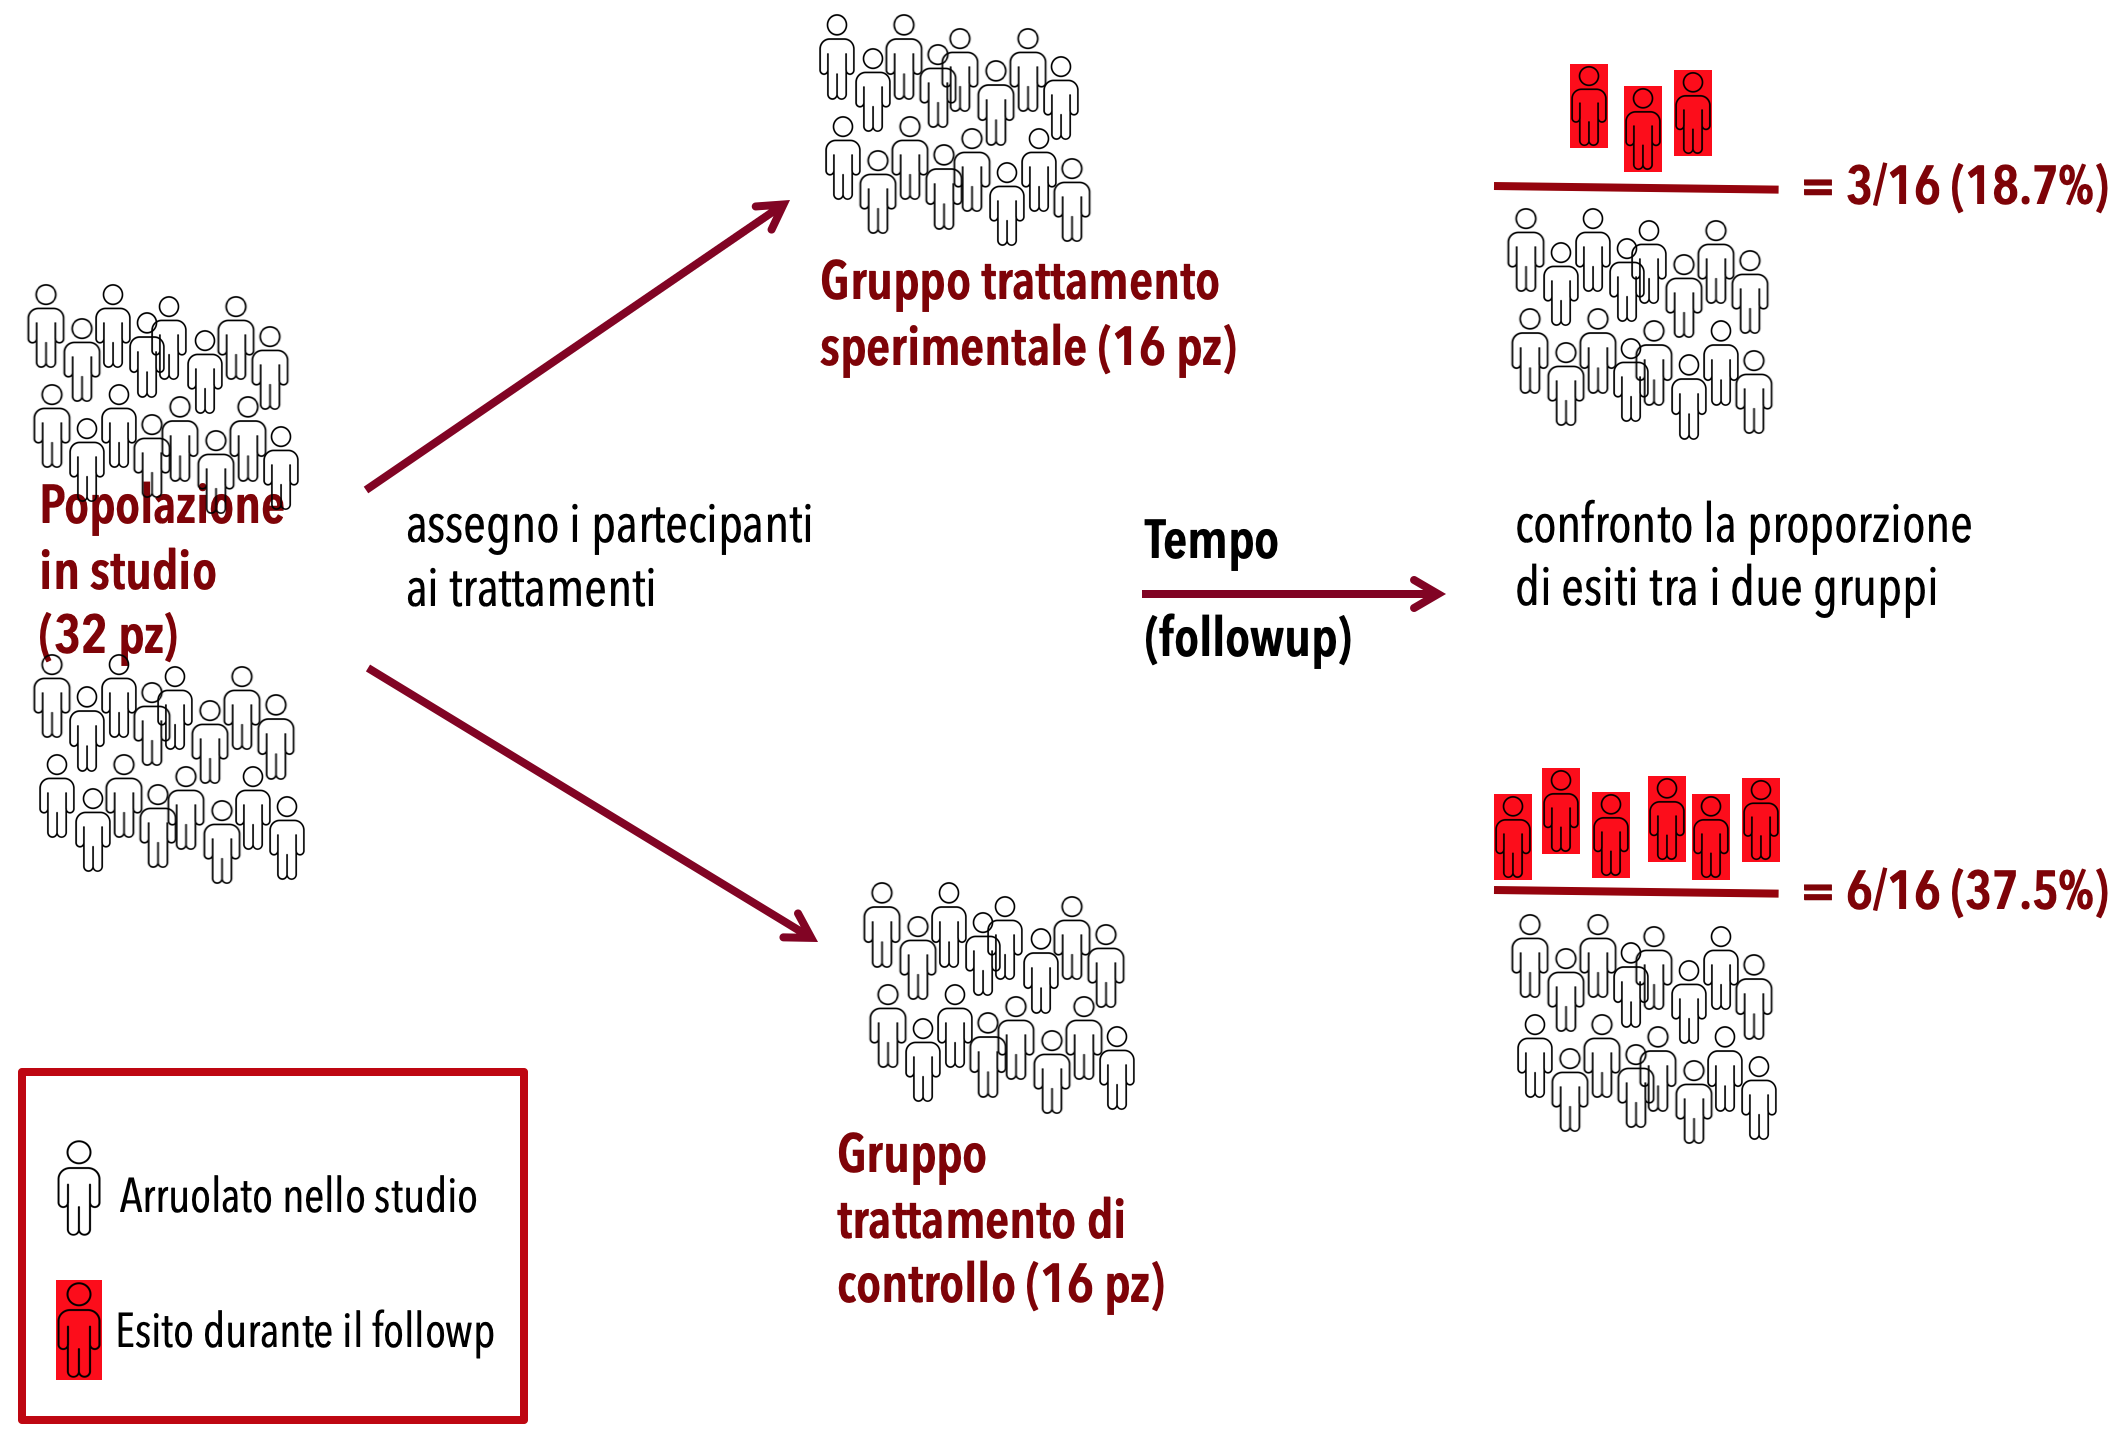
\includegraphics[width=1\textwidth,height=\textheight]{./img/schema-studio-sper.png}

In questo esempio, lo scopo di questo ipotetico studio e' verificare la maggiore efficacia (la «superiorita'») di un trattamento sperimentale rispetto allo standard of care (trattamento di controllo) per la terapia di una determinata patologia. L'esito studiato e' un evento negativo, per es. la morte del paziente.

A partire dalla lista dei pazienti che sono stati selezionati in base a specifici criteri di inclusione, lo sperimentatore assegna casualmente gli individui al gruppo sperimentale o al gruppo di controllo. Dal momento dell'assegnazione ad uno dei due gruppi, inizia il tempo di followup. Durante il followup i pazienti vengono monitorati clinicamente seguento un protocollo predefinito registrando tutti gli esiti, compresi gli eventi avversi di reazione al trattamento. Alla fine del followup si confrontano i due gruppi calcolando in ognuno di essi la proporzione di morti (numero di esiti sul totale dei pazienti che hanno iniziato il followup in quel gruppo).

Ne segue che in questo esempio, il trattamento piu' efficace sara' quello con la minore proporzione di morti. Ovviamente se l'esito studiato fosse stato un evento positivo per la salute (per es. la guarigione), il trattamento piu' efficace sarebbe stato quello che garantische la maggiore proporzione di guariti.

Vengono di seguito accennate alcune caratteristiche generali dei trial clinici.

\textbf{Fasi di un trial}. Un trial solitamente prevede le seguenti fasi: formulazione dell'ipotesi di ricerca e stesura del protocollo particolareggiato dello studio, ottenimento dei fondi e approvazione da parte del comitato etico (analisi rischi e benefici del trattamento sperimentale proposto), arruolamento nello studio in base a criteri prestabiliti (criteri di eleggibilita') e previo consenso informato, allocazione dei partecipanti a uno o più gruppi che ricevono i diversi interventi oggetto del confronto (ed evntuale randomizzazione), monitoraggio degli esiti (incluso gli eventi avversi) durante il followup, confronto tra proporzione degli esiti nei diversi gruppi e pubblicazione dei risultati.

\textbf{Criteri di inclusione (eleggibilità)}. Chi è eleggibile? Il pre-requisito e' che tutti gli individui arruolati possano avere (almeno in teoria) l'esito studiato durante il followup, o come si dice in gergo, siano ``a rischio'' di avere l'esito. Il tipo di popolazione selezionata dipende dagli scopi del trial e deve essere definita a priori. Piu' i criteri sono specifici, migliore e' la precisione del risultato ma minore e' la sua generalizzabilita' ad altri setting assistenziali. E' inoltre molto importante che i pazienti nei due gruppi a confronto abbiano lo stesso livello di prognosi, oltre che ovviamente la stessa malattia. Se per esempio mettessimo tutti i pz gravi nel gruppo sperimentale osserveremo presumibilmente una minore efficacia indipendentemente dalla bonta' o meno del trattamento.

\textbf{Dimensione del campione}. Il campione di individui dovrebbe essere abbastanza ampio da permettere di individuare una differenza di esiti con un potere statistico sufficiente e più sono gli esiti in studio, più individui sono necessari. La dimensione del campione deve essere calcolata in base all'effetto atteso in termini di differenza delle incidenze nei due gruppi ed alla precisione e accuratezza statistica che si vuole raggiungere e inserita nel protocollo sottomesso per l'approvazione del comitato etico.

\textbf{Randomizzazione}. E' l'assegnazione casuale del paziente ad un trattamento. Avviene tramite l'estrazione di numeri casuali. Ne' lo sperimentatore ne' il paziente possono influenzare l'assegnazione al trattamento. Rimuove potenziali bias derivanti dall'assegnazione dei soggetti nei gruppi di trattamento e tende a produrre gruppi confrontabili e intercambiabili, bilanciando (in media) sia i determinanti conosciuti, sia quelli sconosciuti dell'esito. E' molto importante effettuare una corretta randomizzazione che e' una prerogativa degli studi sperimentali.

\textbf{Durata del followup}. La durata del followup dipende dagli obiettivi del trial, dal tipo di trattamento, dalle caratteristiche dei pazienti e dalla patologia ed esito che viene studiato. Puo' andare da pochi giorni fino ad alcuni anni.

\textbf{Effetto placebo}. L'effetto totale osservato in uno studio e' la somma degli effetti del trattamento, del miglioramento spontaneo, della risposta specifica al farmaco e delle risposte aspecifiche soggettive dei pz. Il disegno sperimentale deve essere tale da evidenziare l'effetto del trattamento al netto di tutti gli altri effetti. L'effetto placebo sono la somma degli effetti soggettivi che non sono dovuti alla terapia ma a componenti psicologiche del pz come la fiducia nel medico, nella sperimentazione o nel tipo di terapia. Nei trial sull'efficacia dei farmaci si utilizzava un tempo il placebo: una sostanza farmacologicamente inerte ma identica al farmaco sperimentale. In molti trial moderni il gruppo di confronto riceve un farmaco di confronto (di solito lo standard of care).

\textbf{Mascheramento}. Si attua somministrando il trattamento in «cieco» per evitare interferenza dovute alle aspettative ottimistiche del pz o dello staff implicato nel trial. Al contrario nei trial «aperti» (open label) non c'e' mascheramento sul trattamento somministrato. Il mascheramento puo' essere di tipo:

\begin{itemize}
\item
  \emph{singolo cieco}: i partecipanti non sono a conoscenza a quale gruppo di trattamento sono stati assegnati
\item
  \emph{Doppio cieco}: lo staff che somministra loro il trattamento non è a conoscenza a quale gruppo di trattamento sono stati assegnati
\item
  \emph{Triplo cieco}: lo staff che monitora l`esito non e' a conoscenza a quale gruppo di trattamento i vari pazienti sono stati assegnati. Non e' necessario quando l'outcome si basa su diagnostica strumentale, per gli outcome non oggettivi il problema e' maggiore. A volte puo' essere in cieco anche lo statistico che fa l'analisi.
\end{itemize}

\textbf{Compliance (aderenza al protocollo)}. E' l'aderenza dei partecipanti alle procedure descritte nel protocollo.
Deviazioni dal protocollo possono accadere per alcuni partecipanti a causa di effetti secondari del trattamento. Per questo motivo il pz puo' essere riassegnato per il proseguo dello studio al gruppo di controllo oppure il trattamento puo' venire interrotto). La non compliance rende i due gruppi a confronto più simili, riducendo la capacità dello studio di evidenziare differenze dell'esito del trattamento tra i due gruppi (diminuice la potenza dello studio).

\textbf{Esiti primari ed esiti surrogati}.
Negli studi clinici di solito si utilizzano esiti primari ed esiti secondari (o surogati). Gli esiti primari sono esiti rilevanti clinicamente (morte, ricadute, guarigione\ldots{}) mentre l'esito surrogato: esito che risulta correlato con l'esito primario ma e' piu' semplice (o veloce) da ottenere. Per esempio negli studi sull'incidenza degli esiti cardiovascolari maggiori (infarto, ictus) viene utilizzato come esito surrogato l'ipertensione arteriosa oppure negli studi oncologici invece della morte puo' venire utilizzata la dimensione del tumore. In entrambi i casi l'esito surrogato si verifica prima durante il followup, accorciandone quindi i tempi. Tuttavia, non sempre all'esito surrogato segue temporalmente un esito primario. Per questo motivo sono piu' affidabili e significativi gli studi che verificano l'efficacia dei trattamenti su esiti primari.

\textbf{Aspetti etici e ruolo del comitato etico }. Negli studi sperimentali gli aspetti etici devono sempre essere considerati con il massimo scrupolo. Lo studio viene effettato \emph{solo} se c'e' ragionevole incertezza su quale trattamento scegliere (e.g.~quale trattamento e' più efficace). Il ruolo dei Comitati Etici diventa cruciale nel valutare il protocollo dello studio prima di dare l'autorizzazione. Inoltre il comitato etico effettua un monitoraggio di tutto lo studio, predisponendo delle analisi ad interim durante tutta la durata del trial, per es. a 6, 12 e 18 mesi. Il comitato etico locale recepisce i dettami dell'International Review Board, salvaguardia i diritti e la salute dei pazienti che partecipano allo studio, verifica che i rischi siano ragionevoli in relazione ai benefici attesi, verifica che il consenso informato sia documentato per ogni partecipante allo studio, garantisce l'integrita' scientifica del trial e ne dispone l'eventuale interruzione.

\textbf{Motivi per l'interruzione del trial}. Un trial puo' essere interrotto prima del termine prefissato se c'e' evidenza di maggiore efficacia del trattamento sperimentale nell'analisi ad interim o al contrario se c'e'evidenza di inefficacia, se gli effetti collaterali del trattamento sono troppo gravi per continuare, se il reclutamento dei pazienti troppo lento, se i dati sono di scarsa qualita', se c'e' scarsa compliance (aderenza al protocollo) o troppe perdite al followup.

\textbf{Consenso informato}. Descrive la natura dello studio, i trattamenti, le procedure, i rischi ragionevoli
prevedibili e i benefici attesi. Deve indicare che lo studio e' a fini di ricerca. Deve indicare che la partecipazione non implica perdita di benefici se il paziente rifiuta di partecipare durante lo studio (perdita al follow-up)

\hypertarget{risultati-di-uno-studio-sperimentale}{%
\section{Risultati di uno studio sperimentale}\label{risultati-di-uno-studio-sperimentale}}

Gli esiti clinici (morte, guarigione, ricadute) sono spesso espresse con una variabile dicotomica (si / no, vivo / morto, ecc.). In questo caso, la misura di esito utilizzata in un RCT e' l'incidenza cumulativa (o rischio di sviluppare l'esito) e i risultati sono organizzati in una tabella di contingenza. Nel caso invece che l'esito sia misurato tramite una variabile continua (per es. livelli marcatori ematici, scala infermieristica ecc.), si calcola il valore medio per gruppo.

\hypertarget{tabella-di-contingenza}{%
\subsection{Tabella di contingenza}\label{tabella-di-contingenza}}

Quando l'esito e il trattamento sono quantificati tramite variabili dicotomiche, l'organizzazione dei dati prevede la realizzazione di una tabella 2x2 (due righe x due colonne). Si puo' organizzare le righe e le colonne come si vuole ma un metodo facile da ricordare prevede che:

\begin{itemize}
\item
  la prima riga contenga il \emph{trattamento sperimentale}
\item
  la seconda riga il \emph{trattamento di controllo}
\item
  la prima colonna il numero di \emph{esiti}, ovvero coloro che hanno avuto l'outcome durante il followup
\item
  la seconda colonna il numero di \emph{non esiti}, ovvero coloro che non hanno avuto l'outcome
\end{itemize}

\begin{longtable}[]{@{}llll@{}}
\toprule
Trattamento & Esito & Non Esito & Tot\tabularnewline
\midrule
\endhead
Trattamento Sperimentale & a & b & a+b\tabularnewline
Trattamento Controllo & c & d & c+d\tabularnewline
Tot & a+c & b+d & a+b+c+d\tabularnewline
\bottomrule
\end{longtable}

Cosi' facendo procedendo da sx a dx avreno le seguenti celle (a, b, c, d):

a: numero esiti nel gruppo sperimentale

b: numero di non esiti nel gruppo sperimentale

c: numero esiti nel gruppo controllo

d: numero di non esiti nel gruppo controllo

Il totale della prima riga (a+b) rappresenta la somma dei pazienti che hanno ricevuto il trattamento sperimentale, mentre la somma della seconda riga (c+d) rappresenta la somma dei pazienti che hanno ricevuto il trattamento di controllo. La somma della prima colonna (a+c) rappresenta il totale dei pz che hanno avuto l'esito, la somma della seconda colonna (b+d) coloro che non lo hanno avuto. Il totale dei pz nel trial e' la somma dell 4 celle (a+b+c+d).

\hypertarget{incidenza-di-malattia}{%
\subsection{Incidenza di malattia}\label{incidenza-di-malattia}}

L'incidenza (o rischio) di malattia e' il numero di casi registrati alla fine del follow up rispetto al numero di pz che facevano parte del gruppo all'inizio dello studio.

\[Incidenza = \frac{Numero\ \ casi\ \ durante\ \ followup}{Numero\ \ pz\ \ che\ \ hanno\ \ iniziato \ \  followup}\]

Esprime la probabilita' di avere l'esito durante il followup in una certa popolazione.

Si distinguono:

\begin{quote}
EER (experimental event rate) = incidenza (o rischio) nel gruppo sperimentale

\[EER = \frac{a}{(a+b)}\]

Dove a e' il numero di casi durante il followup nel gruppo sperimentale e (a+b) e' il numero di pz che hanno iniziato il followup nel gruppo sperimentale

CER (control event rate) = incidenza (o rischio) nel gruppo di controllo

\[CER = \frac{c}{(c+d)}\]

Dove c e' il numero di casi durante il followup nel gruppo di controllo e (c+d) e' il numero di pz che hanno iniziato il followup nel gruppo di controllo
\end{quote}

\textbf{Esempio 1}
Viene condotto un ipotetico trial per verificare l'efficacia del trattamento della ferita chirurgica addominale infetta. Il trattamento sperimentale con iodopovidone e' confrontato con il trattamento con clorexidina, l'esito e' la guarigione (remissione dell'infezione del sito chirurgico) alla fine del followup). Nel gruppo iodopovidone iniziano il followup 100 pz, 90 guariscono. Nel gruppo clorexidina iniziano follow up 100 pz, 88 guariscono.
Quale dei due trattamenti sembra piu' efficace?

Formuliamo il quesito di ricerca tramite il metodo PICO

P: pz con ferita addome infetta

I: iodopovidone

C: clorexidina

O: guarigione

Poi realizziamo la tabella di contingenza 2x2

\begin{longtable}[]{@{}llll@{}}
\toprule
Trattamento & Guarigione & Non Guarigione & Tot\tabularnewline
\midrule
\endhead
Iodopovidone & 90 & 10 & 100\tabularnewline
Clorexidina & 88 & 12 & 100\tabularnewline
Tot & 178 & 22 & 200\tabularnewline
\bottomrule
\end{longtable}


\[EER = \frac{90}{100} = 0.9 \ \ (90\%)\]

\[CER = \frac{88}{100} = 0.88 \ \ (88\%)\]

Conclusione: il trattamento piu' efficace sembra quello tramite iodopovidone perche' guariscono il 90\% dei pazienti rispetto a 88\% delle guarigioni che ottengo trattando la ferita con la clorexidina.

\textbf{Esempio 2}
Viene condotto un ipotetico trial per verificare quale trattamento di disinfezione preventiva del sito di inserimento del catetere arterioso sia piu' efficace per la prevenzione delle infezioni (che rappresenta quindi l'esito studiato). Il confronto e' tra soluzione alcolica (trattamento sperimentale) e soluzione saponosa (trattamento di controllo). Alla fine del followup nel gruppo soluzione alcolica su 100 pz, 2 hanno contratto le infezioni durante il followup; nel gruppo soluzione saponosa: inizio follow up 100 pz, 3 infezioni durante il followup. Quale dei due trattamenti sembra piu' efficace?

Formuliamo il quesito di ricerca tramite il metodo PICO

P: pz con catetere arterioso

I: soluzione alcolica

C: soluzione saponosa

O: infezioni

Poi realizziamo la tabella di contingenza 2x2

\begin{longtable}[]{@{}llll@{}}
\toprule
Trattamento & Infezione & Non Infezione & Tot\tabularnewline
\midrule
\endhead
Sol. alcolica & 2 & 97 & 100\tabularnewline
Sol. saponosa & 3 & 98 & 100\tabularnewline
Tot & 5 & 195 & 200\tabularnewline
\bottomrule
\end{longtable}


\[EER = \frac{2}{100} = 0.2 \ \ (2\%)\]

\[CER = \frac{3}{100} = 0.3 \ \ (3\%)\]

Conclusione: il trattamento preventivo piu' efficace sembra quello tramite soluzione alcolica perche' il 2\% dei pazienti contrae un infezione al sito di inserzione del catetere rispetto a 3\% nel gruppo trattato con soluzione saponosa.

\textbf{Esempio 3}
Viene condotto un ipotetico trial per verificare quale trattamento analgesico sia piu' efficace per prevenire il dolore percepito dai bambini che devono essere sottoposto a sutura di una ferita lacero-contuse.
Il confronto e' tra l'applicazione di pomata anestetica (trattamento sperimentale) e somministrazione di lidocaina sottocutanea (trattamento di controllo). L'esito e' misurato mediante una scala di valutazione numerica (NRS, da 0 nessun dolore a 10 dolore molto forte).

Sono reclutati 8 bambini nel gruppo trattato con la pomata anestetica e 10 nel gruppo trattato con lidocaina. I valori della scala NRS dopo l'applicazione del trattamento sono i seguenti:

\begin{longtable}[]{@{}lll@{}}
\toprule
bambino & NRS & trattamento\tabularnewline
\midrule
\endhead
1 & 6 & pomata\tabularnewline
2 & 8 & pomata\tabularnewline
3 & 2 & pomata\tabularnewline
4 & 10 & pomata\tabularnewline
5 & 10 & pomata\tabularnewline
6 & 4 & pomata\tabularnewline
7 & 5 & pomata\tabularnewline
8 & 5 & pomata\tabularnewline
9 & 8 & lidocaina\tabularnewline
10 & 10 & lidocaina\tabularnewline
11 & 7 & lidocaina\tabularnewline
12 & 2 & lidocaina\tabularnewline
13 & 10 & lidocaina\tabularnewline
14 & 3 & lidocaina\tabularnewline
15 & 5 & lidocaina\tabularnewline
16 & 7 & lidocaina\tabularnewline
17 & 5 & lidocaina\tabularnewline
18 & 3 & lidocaina\tabularnewline
\bottomrule
\end{longtable}

Formuliamo il quesito di ricerca tramite il metodo PICO

P: pz pediatrico con ferita lacero-contusa che richiede sutura

I: pomata analgesica

C: lidocaina sottocutanea

O: dolore percepito scala NRS

Si noti che in questo caso l'esito e' quantificato tramite una variabile numerica. Calcoliamo quindi le medie nei due gruppi a confronto.

Media NRS gruppo trattato con la pomata = 6.25

Media NRS gruppo trattato con lidocaina= 6.0

Conclusione: il trattamento con lidocaina sembra essere piu' efficace per rispetto alla pomata per l'analgesia del pz pediatrico che deve essere sottoposto a sutura di una ferita lacero-contusa.


\hypertarget{esercizi-1}{%
\subsection{Esercizi}\label{esercizi-1}}

\textbf{Esercizio 1}
Siete in servizio presso il reparto di pediatria. Un collega vi chiede se un bambino di 4 anni che deve essere sottoposto a sutura di una ferita lacero-contusa, l'applicazione di pomata anestetica sia meno dolorosa della somministrazione di lidocaina sottocutanea per l'analgesia (livello di dolore percepito). Fate la vostra ricerca nella banca dati e trovate uno studio sperimentale nel quale erano stati arruolati 255 bambini \textless{}5 anni con ferita lacero-contusa che dovevano essere sottoposti a sutura. Su ogni bambino veniva effettuata una valutazione del dolore percepito tramite scala VAS. Su 122 trattati con lidocaina, il livello di dolore alto era riportato da 90 di questi. Nel gruppo di controllo, 100 riportavano un alto livello di dolore percepito.

\begin{enumerate}
\def\labelenumi{\arabic{enumi})}
\item
  Definire la tabella di contigenza con l'intestazione di righe e colonne
\item
  Sulla base della tabella calcolare per ciascun gruppo l'incidenza dell'esito
\item
  Quale trattamento sembra essere migliore e perche'?
\end{enumerate}

\textbf{Esercizio 2}
Un collega vi chiede un parere sull'efficacia dei bendaggi a 4 strati (4LB) in aggiunta alla terapia standard rispetto al bendaggio semplice (sempre in aggiunta alla terapia standard) per la medicazione delle ulcere venose aperte alle gambe negli anziani. Fate la vostra ricerca nella banca dati e trovate uno studio sperimentale con un followup di 2 mesi effettuato su pazienti \textgreater{}65 anni d'eta'. Su 215 pazienti che avevano ricevuto il bendaggio 4LB, 77 erano guariti. Nel gruppo di controllo su 209 pazienti, 62 erano guariti.

\begin{enumerate}
\def\labelenumi{\arabic{enumi})}
\item
  Definire la tabella di contigenza con l'intestazione di righe e colonne
\item
  Sulla base della tabella calcolare per ciascun gruppo l'incidenza dell'esito
\item
  Quale trattamento sembra essere migliore e perche'?
\end{enumerate}

\textbf{Esercizio 3}
Un ipotetico studio sperimentale condotto in reparto di medicina con l'obiettivo di valutare l'efficacia della terapia antibiotica locale per prevenire la colonizzazione post-operatoria del sito chirurgico ha riportato i seguenti risultati. Di 32 pz che hanno ricevuto preventivamente l'antibiotico A, 14 hanno riportato colonizzazione della ferita chirurgica. Dei 30 pz che hanno ricevuto preventivamente l'antibiotico B, 12 hanno riportato colonizzazione della ferita chirurgica.

\begin{enumerate}
\def\labelenumi{\arabic{enumi})}
\item
  Definire la tabella di contigenza con l'intestazione di righe e colonne
\item
  Sulla base della tabella calcolare per ciascun gruppo l'incidenza dell'esito
\item
  Quale trattamento sembra essere migliore e perche'?
\end{enumerate}

\hypertarget{misure-di-associazione-tra-trattamento-ed-esito}{%
\subsection{Misure di associazione tra trattamento ed esito}\label{misure-di-associazione-tra-trattamento-ed-esito}}

Per confrontare numericamente i valori di indicenza degli esiti che si misurano nei due gruppi si hanno due opzioni:

\begin{enumerate}
\def\labelenumi{\arabic{enumi}.}
\item
  Calcolare il rapporto di due misure di frequenza dell'evento (una misura per il gruppo sperimentale, l'altra per il gruppo di controllo). In questo caso la misura e' tipicamente l'incidenza.
\item
  Calcolare la differenza di due misure (una misura per il gruppo sperimentale, l'altra per il gruppo di controllo). In questo caso la misura puo' essere l'incidenza o la media (se l'esito e' espresso conuna variabile continua).
\end{enumerate}

\hypertarget{rischio-relativo}{%
\subsection{Rischio relativo}\label{rischio-relativo}}

Il rischio relativo ( \(RR\)) si utilizza quando si confronta l'incidenza dell'esito nel gruppo sperimentale e quello nel gruppo di controllo. Rischio relativo ovvero rapporto dei rischi e':

\[RR = \frac{ EER }{CER}\]

Dove:

EER: Incidenza esito nel gruppo sperimentale

CER: Incidenza esito nel gruppo di controllo

Indica di quante volte è più grande (o piu' piccola) l'incidenza di esito nel gruppo sperimentale rispetto a quella misurata nel gruppo di controllo.

Il rischio relativo assume il valore \(RR=1\) quando l'incidenza di esito nel gruppo sperimentale e' uguale all'incidenza di esito nel gruppo di controllo. In questo caso quindi i due trattamenti hanno \emph{uguale efficacia}.

Se l'esito in studio e' un evento negativo per la salute (per es. la morte) e \(RR>1\), significa che l'incidenza (il rischio) di morte e' piu' alto nel gruppo sperimentale. Concluderemo quindi che il trattamento sperimentale e' \emph{meno efficacie} rispetto a quello di controllo.

Al contrario se l'esito in studio e' un evento positivo per la salute (per es. la guarigione) e \(RR>1\), significa che l'incidenza di guarigione e' piu' alto nel gruppo sperimentale. Concluderemo quindi che il trattamento sperimentale e' \emph{piu' efficace} rispetto a quello di controllo.

\textbf{Interpretazione rischio relativo}. Il richio relativo da informazione sulla ``forza'' della relazione tra esposizione e evento. In altre parole possiamo concludere che i \emph{pazienti del gruppo sperimentale hanno \(RR\) volte la probabilita' di avere l'esito in confronto ai pazienti del gruppo di controllo}. Oppure, in maniera equivalente, che l' \emph{incidenza dell'esito nel gruppo sperimentale e' RR volte quella del gruppo di controllo}.

\textbf{Esempio interpretazione rischio relativo}. Si immagini che un ipotetico studio per verificare l'efficacia di due trattamenti sulla guarigione dei pz ricoverati per una determinata patologia abbia dato i seguenti risultati:

Incidenza di guarigione nel gruppo sperimentale

\(EER = 0.2 = 20\%\)

Incidenza di guarigione nel gruppo di controllo

\(CER= 0.05 = 5\%\)

\[RR = \frac {20}{5} = 4\]

La probabilita' di guarigione con il trattamento sperimentale e' 4 volte quella del trattamento di controllo
ovvero i pz trattati con il trattamento sperimentale (in media) hanno 4 volte la probabilita' di guarire rispetto ai pz trattati con il controllo.

\hypertarget{differenza-dei-rischi}{%
\subsection{Differenza dei rischi}\label{differenza-dei-rischi}}

La differenza dei rischi ( \(RD\)) si utilizza, come il rischio relativo, quando si confronta l'incidenza dell'esito nel gruppo sperimentale e quello nel gruppo di controllo.
Rischio relativo ovvero rapporto dei rischi e':

\[RD = { CER -EER}\]

Dove:

EER: Incidenza esito nel gruppo sperimentale

CER: Incidenza esito nel gruppo di controllo

Indica la differenza in valori assoluti dell'incidenza di esito nel gruppo sperimentale rispetto a quella misurata nel gruppo di controllo.

La differenza dei rischi assume il valore \(RD=0\) quando l'incidenza di esito nel gruppo controllo e' uguale all'incidenza di esito nel gruppo sperimentale. In questo caso quindi i due trattamenti hanno \emph{uguale efficacia}.

Se l'esito in studio e' un evento negativo per la salute (per es. la morte) e \(RD>0\), significa che l'incidenza (il rischio) di morte e' piu' alto nel gruppo di controllo. Concluderemo quindi che il trattamento sperimentale e' \emph{piu' efficace} rispetto a quello di controllo.

Al contrario, se l'esito in studio e' un evento positivo per la salute (per es. la guarigione) e \(RD>0\), significa che l'incidenza di guarigione e' piu' alto nel gruppo di controllo. Concluderemo quindi che il trattamento sperimentale e' \emph{meno efficace} rispetto a quello di controllo.

Si noti che \(RD\) puo' assumere valori negativi (varia tra -inf e +inf).

\textbf{Interpretazione differenza dei rischi}. La differenza dei rischi da informazione sulla differenza assoluta nelle incidenze di evento nei due gruppi a confronto. In altre parole possiamo concludere che i \emph{la differenza dell'incidenza di esito tra il gruppo sperimentale e quello di controllo e' pari a \(RD\) }.

\textbf{Esempio interpretazione differenza dei rischi}. Si immagini che un ipotetico studio per verificare l'efficacia di due trattamenti per prevenire la morte dei pz ricoverati per una determinata patologia abbia dato i seguenti risultati:

Incidenza di morte nel gruppo sperimentale:

\(EER = 5\%\)

Incidenza di morte nel gruppo di controllo:

\(CER= 20\%\)

\[RD = 20\%-5\% = 15\%\]

Quindi la differenza nella probabilita' di morte tra il trattamento sperimentale e quello di controllo e' di 15\% (15 punti percentuale).

\hypertarget{numero-necessario-da-trattare}{%
\subsection{Numero necessario da trattare}\label{numero-necessario-da-trattare}}

Il numero necessario da trattare ( \(NNT\)) e' il numero necessario di soggetti da trattare con il trattamento sperimentale per avere 1 evento favorevole in piu' rispetto al gruppo di controllo:

\[ NNT = \frac{1}{ CER -EER}\]

Si noti che quando CER e EER vengono riportati in percentuale, allora il numeratore della formula e' 100 invece di 1. Il risultato di NNT va sempre arrotondato al numero intero piu' vicino.

\textbf{Esempio interpretazione NNT}. Si immagini che un ipotetico studio per verificare l'efficacia di due trattamenti per prevenire la morte dei pz ricoverati per una determinata patologia abbia dato i seguenti risultati:

Incidenza di morte nel gruppo sperimentale:

\(EER = 15\%\)

Incidenza di guarigione nel gruppo di controllo:

\(CER= 30\%\)

\[NNT = \frac{100}{30-15} = 6.7 = 7\]

Ogni 7 pazienti trattati con il farmaco sperimentale, osservo un evento favorevole in piu' (ovvero una morte in meno) rispetto ai pazienti trattati con il farmaco di controllo.

\hypertarget{differenza-delle-medie}{%
\subsection{Differenza delle medie}\label{differenza-delle-medie}}

Come gia' detto, quando l'esito viene quantificato tramite variabile continua, il confronto tra i due gruppi deve essere effettuato tramite un confronto tra medie. La differenza risultante esprimera' in termini assoluti la differenza nei valori della variabile di esito.

\hypertarget{esempi-1}{%
\subsection{Esempi}\label{esempi-1}}

\textbf{Esempio 1}
Viene condotto un ipotetico trial per verificare l'efficacia del trattamento della ferita chirurgica addominale infetta. Il trattamento con iodopovidone e' confrontato con il trattamento con clorexidina, l'esito e' la guarigione (remissione dell'infezione del sito chirurgico) alla fine del followup. Si ottengono i seguenti valori

\(EER= 90%\)

\(CER= 88%\)

\(RR = \frac{EER} {CER} = \frac{0.9} {0.88} = 1.02\)

La probabilita' di guarigione nei pz trattati con iodopovidone e' 1.02 volte quello dei pz trattati con clorexidina

\(RD = CER – EER = 88\% - 90\% = - 2\%\)

Interpretazione: la differenza delle probabilita' di guarigione tra i pz trattati con iodopovidone e quelli trattati con clorexidina e' del 2\% a favore dello iodopovidone.

Conclusione: il trattamento della ferita chirurgica addominale infetta con iodopovidone sembra essere piu' efficace rispetto all'uso di clorexidina

\textbf{Esempio 2}
Viene condotto un ipotetico trial per verificare quale trattamento di disinfezione preventiva del sito di inserimento del catetere arterioso sia piu' efficace per la prevenzione delle infezioni. Il confronto e' tra soluzione alcolica (trattamento sperimentale) e soluzione saponosa (trattamento di controllo). Si ottengono i seguenti valori:

\(EER= 2\%\)

\(CER= 3\%\)

\(RR = \frac{EER} {CER} = \frac{0.02}{0.03} = 0.66\)

La probabilita' di infezione nei pz trattati con soluzione alcolica e' 0.66 volte quello dei pz trattati con soluz saponosa.

\(RD = CER – EER = 3\%-2\% = 1\%\)

Interpretazione: la differenza delle probabilita' di infezione tra i pz trattati con soluzione alcolica e quelli trattati con sol. saponosa e' del 1\% a favore della soluzione alcolica.

Conclusione: L'uso di soluzione alcolica sembra essere piu' efficace della soluzione saponosa per la disinfezione preventiva del sito di inserimento del catetere arterioso

\textbf{Esempio 3}
Viene condotto un ipotetico trial per verificare quale trattamento analgesico sia piu' efficace per prevenire il dolore percepito dai bambini che devono essere sottoposto a sutura di una ferita lacero-contuse.
Il confronto e' tra l'applicazione di pomata anestetica (trattamento sperimentale) e somministrazione di lidocaina sottocutanea.
L'esito e' misurato mediante una scala di valutazione numerica (NRS, da 0 a 10).

Gruppo pomata: \(media\ \ NRS = 6.25\)
Gruppo lidocaina: \(media\ \ NRS = 6.0\)

\(Differenza \ \ media \ \ trattamenti = 6 – 6.25 = -0.25\)

Interpretazione: la differenza degli score della scala NRS tra i pz trattati con pomata anestetica e quelli trattati con lidocaina e' -0.25.

Conclusione: per l'analgesia dei bambini che devono essere sottoposto a sutura di una ferita lacero-contuse e' piu' efficace l'uso della lidocaina

\hypertarget{esercizi-2}{%
\subsection{Esercizi}\label{esercizi-2}}

\textbf{Esercizio 1}. Lavorate in un reparto di ortopedia. I pazienti operati per inserzione di protesi alle ginocchia vengono dimessi dopo solo tre giorni di degenza (salvo complicazioni). Il capo reparto vi chiede se un intervento tramite telefonata dell'infermiere al pz possa migliorare lo stato di salute fisico precepito ad 1 mese dall'intervento. Nella telefonata l'infermiere puo' informarsi sullo stato della convalescenza, rispondere alle eventuali domande del pz ed indirizzarlo verso le opportune terapie se necessario. Lo stato di salute fisico e' quantificato mediante una scala con score da 0 (pessimo) a 12 punti (ottimo) che viene pero' ricodificata in due sole categorie (stato salute cattivo e stato salute buono).
Alla fine del follow up su 166 pz nel gruppo sperimentale, 120 pz riportavano un buono stato di salute; nel gruppo di controllo su 140 pz, 88 riportavano un buono stato di salute.

\begin{enumerate}
\def\labelenumi{\arabic{enumi})}
\item
  Definire il quesito di ricerca (PICO)
\item
  Definire la tabella di contigenza con l'intestazione di righe e colonne
\item
  Sulla base della tabella calcolare per ciascun gruppo l'incidenza dell'esito
\item
  Calcolare il rischio relativo e la differenza dei rischi
\item
  Interpretare il rischio relativo e la differenza dei rischi
\item
  Quali sono le vostre conclusioni in merito al quesito di ricerca? L'intervento sperimentale e' efficace?
\end{enumerate}

\textbf{Esercizio 2}. L'assistenza casalinga al pz molto anziano, allettato e con diagnosi di demenza viene spesso effettuata da uno dei familiari (care-giver), con possibili conseguenze di stress per lui/lei. Lavorate come infermiere di comunita' e vi chiedete se interventi di supporto mirati al care-giver nella forma di consulti telefonici con personale infermieristico specializzato possano possano diminuire il livello di stress percepito. Lo scopo delle telefonate e' rispondere alle eventuali domande del caregiver sull'assistenza al congiunto, valutare il suo livello di stress ed indirizzarlo verso le opportune terapie se necessario. Arruolate in questo trial 180 care-giver con un followup di 1 anno. A 88 di questi, effettuate 1 telefonata al mese, ed alla fine del followup rilevate un alto livello di stress in 50 caregivers. Nel gruppo di controllo (senza telefonata) misurate alla fine del follow up un alro livello di stress in 66 care givers.

\begin{enumerate}
\def\labelenumi{\arabic{enumi})}
\item
  Definire il quesito di ricerca (PICO)
\item
  Definire la tabella di contigenza con l'intestazione di righe e colonne
\item
  Sulla base della tabella calcolare per ciascun gruppo l'incidenza dell'esito
\item
  Calcolare il rischio relativo e la differenza dei rischi
\item
  Interpretare il rischio relativo e la differenza dei rischi
\item
  Quali sono le vostre conclusioni in merito al quesito di ricerca? L'intervento sperimentale e' efficace?
\end{enumerate}

\textbf{Esercizio 3}. Siete un infermiere di famiglia. Volete valutare l'efficacia di un intervento informativo sui ragazzi tra 12 e i 14 anni per la prevenzione delle malattie sessualmente trasmesse (MST). Decidete di fare un trial di comunita'. In una scuola e in alcune classi estratte a caso effettuate l'intervento mentre in altre no. Due mesi dopo l'intervento misurate tramite questionario l'attitudine ai corretti comportamenti preventivi verso le MST (esito: punteggio scala numerica da 0=scorrette a 10=corrette). Avete ottenuto i seguenti dati:

Gruppo che ha ricevuto l'intervento educativo: numero ragazzi = 50, media punteggio = 3.2

Gruppo di confronto: numero ragazzi = 50, media punteggio = 2.8

\begin{enumerate}
\def\labelenumi{\arabic{enumi})}
\item
  Definire il quesito di ricerca (PICO)
\item
  Calcolare la differenza nell'effetto del trattamento
\item
  Interpretare la differenza nell'effetto del trattamento
\item
  Quali sono le vostre conclusioni in merito al quesito di ricerca? L'intervento educativo e' efficace?
\end{enumerate}

\hypertarget{validita-interna-di-uno-studio}{%
\section{Validita' interna di uno studio}\label{validita-interna-di-uno-studio}}

Quando leggiamo i risultati di uno studio dobbiamo poter valutare la validita' e precisione della stima dell'associazione tra trattamento ed esito. La maggiore (o minore) efficacia del trattamento sperimentale rispetto a quello di controllo si basa sul valore della misura di associazione (il rischio relativo RR o la differenza dei rischi RD) che viene ottenuta su un campione estratto dalla popolazione di pazienti. Ma quanto e' affidabile e preciso questo risultato? Dobbiamo dotarci di un metodo che ci permetta di capire quanto e' affidabile il valore di RR (o quello di RD) ottenuto dal campione, ovvero quanto esso sia vicino al valore che misurerei nell'ipotetico caso che potessi includere nello studio l'intera popolazione (teoricamente infinita) di possibili pazienti. In particolare, vorremo evitare di sbagliare nel concludere che un trattamento e' piu' efficace dell'altro quando invece questo non e' vero.

\hypertarget{intervallo-di-confidenza-ic}{%
\subsection{Intervallo di confidenza (IC)}\label{intervallo-di-confidenza-ic}}

Chiamiamo \emph{parametro} il valore di RR (o di RD) che quantifica l'associazione tra trattamento e esito nella popolazione (teoricamente infinita) dalla quale noi abbiamo estratto il campione di pz che abbiamo incluso nello studio. Su questo campione abbiamo ottenuto una \emph{stima} del RR. La nostra ambizione pero' e' estendere le conclusioni dello studio a tutti i pazienti che fanno parte della popolazione, cioe' applicare il trattamento piu' efficace su tutti i pz affetti da quella patologia. Vorremmo quindi conoscere il valore dell'associazione tra trattamento ed esito nella popolazione (il \emph{parametro}) senza pero' poterla misurare direttamente ma soltanto basandoci sul nostro campione di pazienti.

Quanto la \emph{stima} del RR ottenuta sul campione e' vicina al RR (sconosciuto) della popolazione da cui il campione e' stato estratto? Non possiamo saperlo ma \emph{sui dati del campione} possiamo calcolare un intervallo di valori all'interno del quale siamo ragionevolemente certi che esso ricada. L'\emph{intervallo di confidenza (IC)} indica, con un certo grado di certezza (di solito 95\%), i valori entro i quali il parametro della popolazione, che tentiamo di stimare con il nostro campione e che non potremmo mai misurare, e' compreso. Lo stesso ragionamento esposto sopra e' valido anche per la differenza dei rischi RD.

Quando quantifichiamo l'associazione tra esposizione ed esito usando il rischio relativo, se il valore nullo \(RR=1\) e' compreso nell'intervallo, allora \emph{non} possiamo escludere che il parametro della popolazione da cui e
estratto il campione sia proprio 1. Conseguentemente, non possiamo essere certi della maggiore o minore efficacia del trattamento sperimentale rispetto a quello di controllo.

Allo stesso modo utilizzando la differenza dei rischi, se il valore nullo della misura di associazione \(RD = 0\) e' compreso nell'intervallo, allora non possiamo escludere che il parametro della popolazione sia proprio 0. Ne segue che non possiamo essere certi della maggiore o minore efficacia del trattamento sperimentale rispetto a quello di controllo.

L'intervallo di confidenza ha anche una seconda caratteristica molto utile: ci dice anche quanto la stima ottenuta sul campione e' precisa. Tanto piu' ampio e' l'intervallo di confidenza, quanto piu' la stima ottenuta sul campione sara' imprecisa. Al contrario, minore è l'ampiezza dell'intervallo di confidenza, più precisa sara' la nostra stima puntuale (ovvero minore e' la variazione casuale dei nostri dati).

Interpretazione efficacia del trt sperimentale rispetto al trt di controllo

\begin{longtable}[]{@{}llll@{}}
\toprule
\begin{minipage}[b]{0.22\columnwidth}\raggedright
Esito\strut
\end{minipage} & \begin{minipage}[b]{0.22\columnwidth}\raggedright
Associazione\strut
\end{minipage} & \begin{minipage}[b]{0.22\columnwidth}\raggedright
Intervallo di confidenza\strut
\end{minipage} & \begin{minipage}[b]{0.22\columnwidth}\raggedright
Efficacia del trt sperimentale rispetto al controllo\strut
\end{minipage}\tabularnewline
\midrule
\endhead
\begin{minipage}[t]{0.22\columnwidth}\raggedright
Morte\strut
\end{minipage} & \begin{minipage}[t]{0.22\columnwidth}\raggedright
RR=1.05\strut
\end{minipage} & \begin{minipage}[t]{0.22\columnwidth}\raggedright
1.01 ; 1.10\strut
\end{minipage} & \begin{minipage}[t]{0.22\columnwidth}\raggedright
Minore efficacia\strut
\end{minipage}\tabularnewline
\begin{minipage}[t]{0.22\columnwidth}\raggedright
Ricadute\strut
\end{minipage} & \begin{minipage}[t]{0.22\columnwidth}\raggedright
RR= 0.9\strut
\end{minipage} & \begin{minipage}[t]{0.22\columnwidth}\raggedright
0.8 ; 1.45\strut
\end{minipage} & \begin{minipage}[t]{0.22\columnwidth}\raggedright
uguale\strut
\end{minipage}\tabularnewline
\begin{minipage}[t]{0.22\columnwidth}\raggedright
Morte\strut
\end{minipage} & \begin{minipage}[t]{0.22\columnwidth}\raggedright
RR= 0.80\strut
\end{minipage} & \begin{minipage}[t]{0.22\columnwidth}\raggedright
0.7, 0.9\strut
\end{minipage} & \begin{minipage}[t]{0.22\columnwidth}\raggedright
Maggiore efficacia\strut
\end{minipage}\tabularnewline
\begin{minipage}[t]{0.22\columnwidth}\raggedright
Guarigione\strut
\end{minipage} & \begin{minipage}[t]{0.22\columnwidth}\raggedright
RD= -1.2\strut
\end{minipage} & \begin{minipage}[t]{0.22\columnwidth}\raggedright
-1.4; -0.8\strut
\end{minipage} & \begin{minipage}[t]{0.22\columnwidth}\raggedright
Maggiore efficacia\strut
\end{minipage}\tabularnewline
\begin{minipage}[t]{0.22\columnwidth}\raggedright
Infezioni\strut
\end{minipage} & \begin{minipage}[t]{0.22\columnwidth}\raggedright
RD= 1.2\strut
\end{minipage} & \begin{minipage}[t]{0.22\columnwidth}\raggedright
-0.4 ; 2\strut
\end{minipage} & \begin{minipage}[t]{0.22\columnwidth}\raggedright
uguale\strut
\end{minipage}\tabularnewline
\begin{minipage}[t]{0.22\columnwidth}\raggedright
Guarigione\strut
\end{minipage} & \begin{minipage}[t]{0.22\columnwidth}\raggedright
RD= -2.0\strut
\end{minipage} & \begin{minipage}[t]{0.22\columnwidth}\raggedright
-3.5, 0.5\strut
\end{minipage} & \begin{minipage}[t]{0.22\columnwidth}\raggedright
uguale\strut
\end{minipage}\tabularnewline
\bottomrule
\end{longtable}

\hypertarget{bias}{%
\subsection{Bias}\label{bias}}

Errore sistematico che comporta una stima incorretta o non valida della misura dell'associazione tra esposizione e outcome. E' commesso dallo sperimentatore(Non si puo' correggere (o diminuire) a posteriori

Principali bias dei trial

\begin{longtable}[]{@{}lll@{}}
\toprule
\begin{minipage}[b]{0.30\columnwidth}\raggedright
Tipo di bias\strut
\end{minipage} & \begin{minipage}[b]{0.30\columnwidth}\raggedright
Descrizione\strut
\end{minipage} & \begin{minipage}[b]{0.30\columnwidth}\raggedright
Perche'\strut
\end{minipage}\tabularnewline
\midrule
\endhead
\begin{minipage}[t]{0.30\columnwidth}\raggedright
selezione (partecipazione)\strut
\end{minipage} & \begin{minipage}[t]{0.30\columnwidth}\raggedright
Differenze tra i due gruppi delle caratteristiche dei pz al baseline\strut
\end{minipage} & \begin{minipage}[t]{0.30\columnwidth}\raggedright
scorretta randomizzazione\strut
\end{minipage}\tabularnewline
\begin{minipage}[t]{0.30\columnwidth}\raggedright
informazione (accertamento)\strut
\end{minipage} & \begin{minipage}[t]{0.30\columnwidth}\raggedright
Differenze sistematiche nel modo con cui il trattamento e' amministrato o nella misura dell'outcome\strut
\end{minipage} & \begin{minipage}[t]{0.30\columnwidth}\raggedright
scorretto mascheramento\strut
\end{minipage}\tabularnewline
\begin{minipage}[t]{0.30\columnwidth}\raggedright
selezione (violazione protocollo)\strut
\end{minipage} & \begin{minipage}[t]{0.30\columnwidth}\raggedright
Differenze nelle caratterische dei pz che si ritirano dallo studio o cambiano gruppo o non aderiscono alprotocollo\strut
\end{minipage} & \begin{minipage}[t]{0.30\columnwidth}\raggedright
Perdite al follow up o switch o non aderenza al trattamento differenziale tra i due gruppi\strut
\end{minipage}\tabularnewline
\begin{minipage}[t]{0.30\columnwidth}\raggedright
informazione (reporting)\strut
\end{minipage} & \begin{minipage}[t]{0.30\columnwidth}\raggedright
Differenze sistematiche nel reporting dei risultati (es. riporto solo risultati positivi)\strut
\end{minipage} & \begin{minipage}[t]{0.30\columnwidth}\raggedright
Reporting selettivo\strut
\end{minipage}\tabularnewline
\bottomrule
\end{longtable}

\textbf{Scorretta randomizzazione}. E' un esempio di bias di selezione. Si immagini di avere pz eleggibili al trial con diversa fragilita' clinica: una randomizzazione non corretta porta alla formazione gruppi non omogenei per condizioni cliniche, comorbidita', eta', sesso ecc. Se per esempio una maggiore quota di pz fragili fosse assegnata al gruppo che riceve il trattamento di controllo, potremmo avere una maggiore efficacia del trattamento sperimentale non dovuta' alla bonta' del trattamento ma alla diversa composizione dei gruppi. L'effetto del trattamento sperimentale sara' quindi confuso da tutte le altre variabili che possono influenzare l'esito. Una corretta procedura di randomizzazione e' tale che l'assegnazione di un certo pz ad un gruppo e' casuale e quindi non puo' essere nota in anticipo agli operatori.

\textbf{Scorretto o assenza di mascheramento}. Conoscere il trattamento (se sperimentale o controllo) che viene amministrato ai pz causa un errore sistematico nella somministrazione del trattamento e nell'accertamento dell'esito che dipende dalle aspettative ottimistiche dello staff che compie il trial. A questo si aggiunge l'effetto placebo del pz. Per questo motivo il trattamento assegnato al pz non dovrebbe essere riconoscibile. Ovviamente, se per la somministrazione di farmaci spesso il mascheramento e' possibile per altri interventi assistenziali no.

\textbf{Perdite al followup, non compliance, switch}. E' un esempio di bias di selezione. Si verifica quando le perdite al followup sono differenziali (maggiore in un gruppo rispetto all'altro) oppure la non aderenza al protocollo (compliance) o il passaggio da un gruppo all'altro (switch) riguardano in maniera maggiore uno dei due trattamenti.Per giudicare quanto questo fenomeno possa influire sui risultati, deve essere presente nella pubblicazione una descrizione del numero di soggetti che hanno abbandonato il followup, non compliant e che hanno effettuato lo switch.

\hypertarget{tipi-di-analisi}{%
\subsection{Tipi di analisi}\label{tipi-di-analisi}}

\textbf{Analisi secondo intenzione al trattamento (``intention to treat'')}. In questa tipologia di analisi del dato di un trial l'incidenza di esito nei due gruppi viene calcolata usando al denominatore tutti gli individui che hanno iniziato il followup in un certo gruppo.

\(EER = \frac {esiti\ \ gruppo \ \ sperimentale}{pz \ \ gruppo \ \ sperimentale}\)

\(CER = \frac {esiti\ \ gruppo \ \ controllo}{pz \ \ gruppo \ \ controllo}\)

\textbf{Analisi secondo protocollo (``per protocol'')} In questa tipologia di analisi del dato di un trial l'incidenza di esito nei due gruppi viene calcolata usando al denominatore solo i soggetti che hanno concluso il followup all'interno del gruppo al quale erano stati assegnati. Si escludono dal calcolo sia del numeratore sia del denominatore i pz persi al followup, quelli non aderenti al protocollo e coloro che hanno cambiato gruppo.

\(EER = \frac {esiti\ \ gruppo \ \ sperimentale}{pz \ \ gruppo \ \ sperimentale^1}\)

\(CER = \frac {esiti\ \ gruppo \ \ controllo}{pz \ \ gruppo \ \ controllo^1}\)

\emph{(1) solo pz che hanno finito il follow up seguendo il protocollo nel gruppo di assegnazione}

L'analisi intention to treat e' preferibile perche' rispetta l'assegnazione casuale dei pz ai due gruppi, garantendo quindi l'assenza di bias di selezione e produce stime vicine alla realtà (ci saranno sempre dei non compliant). Tuttavia, tende a sottostimare l'effetto del trattamento. L'analisi secondo protocollo non rispetta l'assegnazione casuale ma produce stime accurate nel sottogruppo di popolazione che ha seguito il protocollo. Tende a sovrastimare l'effetto trattamento

\hypertarget{valutazione-critica-rct-critical-appraisal}{%
\section{Valutazione critica RCT (critical appraisal)}\label{valutazione-critica-rct-critical-appraisal}}

In generale gli studi sperimentali sono il modello preferibile per la sperimentazione clinica e, nello specifico, sono i piu' efficienti ed affidabili quando i quesiti assistenziali che rigurdano l'efficacia dei trattamenti infermieristici. I \textbf{vantaggi} degli studi sperimentali comprendono: 1) sono gli studi che se ben condotti sono più corretti da un punto di vista metodologico; 2) costituiscono gli unici modelli di studio in grado di stabilire l'efficacia degli interventi; 3) se ben condotti non sono suscettibili a bias di selezione, di classificazione e di confondimento. Tra gli \textbf{svantaggi} ricordiamo: 1) problemi etici; 2) lunga durata, costi elevati, difficoltà organizzative; 3) Problemi di validita' esterna: non sempre il risultato di questa procedura controllata in ogni sua fase e' applicabile al setting assistenziale in condizioni di ``real life''.

Quando esaminiamo uno studio dobbiamo valutarlo criticamente in termini di validita' interna, significativita' clinica e applicabilita'. In altri termini dobbiamo verificare non solo che uno studia sia corretto dal punto di vista delle metodologie (come e' stato condotto) ma anche che sia affidabile e rilevante (faccia la differenza) in merito al quesito assistenziale.

E' importante effettuare una valutazione critica secondo lo schema seguente.

\begin{longtable}[]{@{}lll@{}}
\toprule
\begin{minipage}[b]{0.30\columnwidth}\raggedright
Cosa dobbiamo capire\strut
\end{minipage} & \begin{minipage}[b]{0.30\columnwidth}\raggedright
Indicatore\strut
\end{minipage} & \begin{minipage}[b]{0.30\columnwidth}\raggedright
come\strut
\end{minipage}\tabularnewline
\midrule
\endhead
\begin{minipage}[t]{0.30\columnwidth}\raggedright
Lo studio e' valido?\strut
\end{minipage} & \begin{minipage}[t]{0.30\columnwidth}\raggedright
Assenza di bias\strut
\end{minipage} & \begin{minipage}[t]{0.30\columnwidth}\raggedright
Controllo le metodologie utilizzate\strut
\end{minipage}\tabularnewline
\begin{minipage}[t]{0.30\columnwidth}\raggedright
E' significativo dal punto di vista clinico?\strut
\end{minipage} & \begin{minipage}[t]{0.30\columnwidth}\raggedright
Effetto del trattamento fa la differenza in termini clinici (non statistici)\strut
\end{minipage} & \begin{minipage}[t]{0.30\columnwidth}\raggedright
Esamino la grandezza del RR e RD e l'intervallo di confidenza\strut
\end{minipage}\tabularnewline
\begin{minipage}[t]{0.30\columnwidth}\raggedright
Le conclusioni sull'efficacia del trattamento sono applicabili ai miei pz?\strut
\end{minipage} & \begin{minipage}[t]{0.30\columnwidth}\raggedright
Quanto la popolazione studiata e' simile alla mia\strut
\end{minipage} & \begin{minipage}[t]{0.30\columnwidth}\raggedright
Rifletto se il trattamento e le metodologie sono applicabili al mio setting assistenziale\strut
\end{minipage}\tabularnewline
\bottomrule
\end{longtable}

\textbf{Validita' interna}. Consiste nel verificare, esaminando la sezione dei methods della pubblicazione, l'assenza di bias. Cosa devo chiedermi quando leggo il lavoro:
- l'assegnazione dei pz al trattamento era randomizzata?
- la randomizzazione era ``nascosta'' agli operatori?
- i gruppi erano simili all'inizio dello studio?
- Il follow up era sufficientemente lungo e completo?
- l'analisi e' stata eseguita secondo intention to treat?
- il mascheramento e' stato effettuato?

\textbf{Significativita' clinica}. Consiste nel verificare, esaminando la sezione results della pubblicazione, quanto siano affidabili i risultati:
- la dimensione dell'effetto del trattamento e' clinicamente rilevante?
- quanto e' precisa la stima del trattamento?
- e' stato utilizzato un esito clinico o un esito surrogato?
- i benefici della terapia superano gli eventuali danni?

\textbf{Applicabilita' clinica}
Consiste nel verificare, esaminando la sezione discussion della pubblicazione, quanto siano generalizzabili i risultati. Ovvero si deve riflettere se l'intervento che risulta piu' efficace nello studio sia poi applicabile e mantenga le proprie prerogative di maggiore efficacia anche in altri setting assistenziali ed in condizioni di real life. Sono aspetti da considerare:
- il mio pz e' sufficientemente simile a quelli considerati nello studio?
- il trattamento e' attuabile nel mio contesto lavorativo?
- il trattamento e' attuabile al mio pz, tenuto conto delle sue preferenze e aspettative?
- posso estrapolarne i risultati e applicarli al mio posto di lavoro?

\textbf{Valutazione critica RCT- check list}
Le check list sono molto utili durante la lettura per fare un sommario dei punti di forza e delle debolezze di uno studio. Di seguito, a titolo di esempio, e' riportata un checklist semplificata. Si legge lo studio e si risponde alle seguenti domande (critical appraisal) con si/no/non riportato (nr):

\begin{longtable}[]{@{}lr@{}}
\toprule
\begin{minipage}[b]{0.47\columnwidth}\raggedright
Domanda\strut
\end{minipage} & \begin{minipage}[b]{0.47\columnwidth}\raggedleft
Risposta (barrare ove appropriato)\strut
\end{minipage}\tabularnewline
\midrule
\endhead
\begin{minipage}[t]{0.47\columnwidth}\raggedright
1.Lo studio si basa su un quesito valido (es. riconducibile al PICO)?\strut
\end{minipage} & \begin{minipage}[t]{0.47\columnwidth}\raggedleft
SI / NO / Non riportato\strut
\end{minipage}\tabularnewline
\begin{minipage}[t]{0.47\columnwidth}\raggedright
\strut
\end{minipage} & \begin{minipage}[t]{0.47\columnwidth}\raggedleft
\strut
\end{minipage}\tabularnewline
\begin{minipage}[t]{0.47\columnwidth}\raggedright
2. Gli autori usano un tipo di studio adeguato al quesito?\strut
\end{minipage} & \begin{minipage}[t]{0.47\columnwidth}\raggedleft
SI / NO / Non riportato\strut
\end{minipage}\tabularnewline
\begin{minipage}[t]{0.47\columnwidth}\raggedright
\strut
\end{minipage} & \begin{minipage}[t]{0.47\columnwidth}\raggedleft
\strut
\end{minipage}\tabularnewline
\begin{minipage}[t]{0.47\columnwidth}\raggedright
\textbf{3. VALIDITA'}\strut
\end{minipage} & \begin{minipage}[t]{0.47\columnwidth}\raggedleft
\strut
\end{minipage}\tabularnewline
\begin{minipage}[t]{0.47\columnwidth}\raggedright
3.1 Il gruppo sperimentale ed il gruppo di controllo sono simili in termini di prognosi all'inizio dello studio?\strut
\end{minipage} & \begin{minipage}[t]{0.47\columnwidth}\raggedleft
SI / NO / Non riportato\strut
\end{minipage}\tabularnewline
\begin{minipage}[t]{0.47\columnwidth}\raggedright
3.2 l'assegnazione dei pazienti ai gruppi era randomizzata?\strut
\end{minipage} & \begin{minipage}[t]{0.47\columnwidth}\raggedleft
SI / NO / Non riportato\strut
\end{minipage}\tabularnewline
\begin{minipage}[t]{0.47\columnwidth}\raggedright
3.3 mascheramento della procedura di randomizzazione?\strut
\end{minipage} & \begin{minipage}[t]{0.47\columnwidth}\raggedleft
SI / NO / Non riportato\strut
\end{minipage}\tabularnewline
\begin{minipage}[t]{0.47\columnwidth}\raggedright
3.4 e' seguita l'analisi intention to treat (ovvero considerando tutti i soggetti presenti all'inizio del trial)?\strut
\end{minipage} & \begin{minipage}[t]{0.47\columnwidth}\raggedleft
SI / NO / Non riportato\strut
\end{minipage}\tabularnewline
\begin{minipage}[t]{0.47\columnwidth}\raggedright
3.5 i gruppi erano simili per tutti i fattori conosciuti (tranne ovviamente il trattamento)?\strut
\end{minipage} & \begin{minipage}[t]{0.47\columnwidth}\raggedleft
SI / NO / Non riportato\strut
\end{minipage}\tabularnewline
\begin{minipage}[t]{0.47\columnwidth}\raggedright
3.6 mantenevano la stessa prognosi anche dopo l'avvio dello studio?\strut
\end{minipage} & \begin{minipage}[t]{0.47\columnwidth}\raggedleft
SI / NO / Non riportato\strut
\end{minipage}\tabularnewline
\begin{minipage}[t]{0.47\columnwidth}\raggedright
3.7 pazienti in cieco (singolo cieco)?\strut
\end{minipage} & \begin{minipage}[t]{0.47\columnwidth}\raggedleft
SI / NO / Non riportato\strut
\end{minipage}\tabularnewline
\begin{minipage}[t]{0.47\columnwidth}\raggedright
3.8 somministratori del trattamento in cieco (doppio cieco)?\strut
\end{minipage} & \begin{minipage}[t]{0.47\columnwidth}\raggedleft
SI / NO / Non riportato\strut
\end{minipage}\tabularnewline
\begin{minipage}[t]{0.47\columnwidth}\raggedright
3.9 analisti in cieco (triplo cieco)?\strut
\end{minipage} & \begin{minipage}[t]{0.47\columnwidth}\raggedleft
SI / NO / Non riportato\strut
\end{minipage}\tabularnewline
\begin{minipage}[t]{0.47\columnwidth}\raggedright
3.10 il follow up era completo?\strut
\end{minipage} & \begin{minipage}[t]{0.47\columnwidth}\raggedleft
SI / NO / Non riportato\strut
\end{minipage}\tabularnewline
\begin{minipage}[t]{0.47\columnwidth}\raggedright
\strut
\end{minipage} & \begin{minipage}[t]{0.47\columnwidth}\raggedleft
\strut
\end{minipage}\tabularnewline
\begin{minipage}[t]{0.47\columnwidth}\raggedright
\textbf{4. RISULTATI} Calcolare per ogni esito (endpoint)\strut
\end{minipage} & \begin{minipage}[t]{0.47\columnwidth}\raggedleft
\strut
\end{minipage}\tabularnewline
\begin{minipage}[t]{0.47\columnwidth}\raggedright
4.1 Rischio gruppo trattato\strut
\end{minipage} & \begin{minipage}[t]{0.47\columnwidth}\raggedleft
\strut
\end{minipage}\tabularnewline
\begin{minipage}[t]{0.47\columnwidth}\raggedright
4.2 Rischio gruppo confronto\strut
\end{minipage} & \begin{minipage}[t]{0.47\columnwidth}\raggedleft
\strut
\end{minipage}\tabularnewline
\begin{minipage}[t]{0.47\columnwidth}\raggedright
4.3 Differenza del rischio (con IC95\%)\strut
\end{minipage} & \begin{minipage}[t]{0.47\columnwidth}\raggedleft
\strut
\end{minipage}\tabularnewline
\begin{minipage}[t]{0.47\columnwidth}\raggedright
4.4 Rapporto dei rischi (con IC95\%)\strut
\end{minipage} & \begin{minipage}[t]{0.47\columnwidth}\raggedleft
\strut
\end{minipage}\tabularnewline
\begin{minipage}[t]{0.47\columnwidth}\raggedright
4.5 NNT\strut
\end{minipage} & \begin{minipage}[t]{0.47\columnwidth}\raggedleft
\strut
\end{minipage}\tabularnewline
\begin{minipage}[t]{0.47\columnwidth}\raggedright
\strut
\end{minipage} & \begin{minipage}[t]{0.47\columnwidth}\raggedleft
\strut
\end{minipage}\tabularnewline
\begin{minipage}[t]{0.47\columnwidth}\raggedright
\textbf{5. APPLICABILITA' DEI RISULTATI}\strut
\end{minipage} & \begin{minipage}[t]{0.47\columnwidth}\raggedleft
\strut
\end{minipage}\tabularnewline
\begin{minipage}[t]{0.47\columnwidth}\raggedright
5.1 I pazienti dello studio sono simili a quelli che riscontro in ambito clinico?\strut
\end{minipage} & \begin{minipage}[t]{0.47\columnwidth}\raggedleft
SI / NO / Non riportato\strut
\end{minipage}\tabularnewline
\begin{minipage}[t]{0.47\columnwidth}\raggedright
5.2 Gli outcome considerati sono clinicamente rilevanti?\strut
\end{minipage} & \begin{minipage}[t]{0.47\columnwidth}\raggedleft
SI / NO / Non riportato\strut
\end{minipage}\tabularnewline
\begin{minipage}[t]{0.47\columnwidth}\raggedright
5.3 I benefici bilanciano i danni e i potenziali costi?\strut
\end{minipage} & \begin{minipage}[t]{0.47\columnwidth}\raggedleft
SI / NO / Non riportato\strut
\end{minipage}\tabularnewline
\begin{minipage}[t]{0.47\columnwidth}\raggedright
\strut
\end{minipage} & \begin{minipage}[t]{0.47\columnwidth}\raggedleft
\strut
\end{minipage}\tabularnewline
\begin{minipage}[t]{0.47\columnwidth}\raggedright
\textbf{6. CONCLUSIONI}\strut
\end{minipage} & \begin{minipage}[t]{0.47\columnwidth}\raggedleft
\strut
\end{minipage}\tabularnewline
\begin{minipage}[t]{0.47\columnwidth}\raggedright
6.1 Lo studio ha un quesito ed un disegno appropriato?\strut
\end{minipage} & \begin{minipage}[t]{0.47\columnwidth}\raggedleft
SI / NO / Non riportato\strut
\end{minipage}\tabularnewline
\begin{minipage}[t]{0.47\columnwidth}\raggedright
6.2 Lo studio ha validita' interna soddisfacente?\strut
\end{minipage} & \begin{minipage}[t]{0.47\columnwidth}\raggedleft
SI / NO / Non riportato\strut
\end{minipage}\tabularnewline
\begin{minipage}[t]{0.47\columnwidth}\raggedright
6.3 I risultati dello studio sono significativi dal punto di vista clinico?\strut
\end{minipage} & \begin{minipage}[t]{0.47\columnwidth}\raggedleft
SI / NO / Non riportato\strut
\end{minipage}\tabularnewline
\begin{minipage}[t]{0.47\columnwidth}\raggedright
6.4 I risultati sono applicabili nella pratica quotidiana?\strut
\end{minipage} & \begin{minipage}[t]{0.47\columnwidth}\raggedleft
SI / NO / Non riportato\strut
\end{minipage}\tabularnewline
\bottomrule
\end{longtable}

\hypertarget{esercizio-2}{%
\subsection{Esercizio}\label{esercizio-2}}

Leggere criticamente lo studio \emph{Efficacia della medicazione sterile trasparente per il fissaggio del catetere venoso periferico (CVP) sull'incidenza delle flebiti rispetto all'uso della medicazione standard: un trial randomizzato e controllato} e compilare la scheda di valutazione critica (con si/no o calcolando i valori tramite OpenEpi)



\hypertarget{studi-di-prognosi-e-studi-eziologici}{%
\chapter{Studi di prognosi e studi eziologici}\label{studi-di-prognosi-e-studi-eziologici}}

L'obiettivo degli \emph{studi di prognosi} e' individuare quali caratteristiche del paziente con una certa diagnosi siano associate con gli esiti durante il decorso della malattia. Questi fattori, come per es. l'eta', la storia clinica, le caratteristiche della malattia (es. stadio del tumore), eventuali comorbidita' ecc. si dicono \emph{fattori prognostici}. Per esempio: e' il livello pressione intracranica pz ricoverati per trauma cranico associato con morte? E' il braden score piu' elevato associato con lesioni da pressione nel pz ricoverato in terapia intensiva? I fattori prognostici non devono necessariamente causare l'esito ma devono essere in grado di predirlo con un certo grado di approssimazione.

L'obiettivo degli \emph{studi eziologici} e' individuare quali caratteristiche degli individui all'interno di una popolazione siano associate con il rischio di un certo esito. Queste caratteristiche come per esempio il livello di colesterolo, l'obesita', il fumo di sigaretta ecc. si dicono fattori di rischio. Per esempio: e' una certa dieta collegata con lo sviluppo di obesita' negli adolescenti? Le donne immigrate sono piu' a rischio di non effettuare screening oncologici? e' il bere alcolici compulsivamente (binge) un comportamento a rischio per le malattie sessualmente trasmesse?

Quindi le principali differenze tra uno studio prognostico ed uno eziologico sono:

\begin{itemize}
\item
  I partecipanti sono differenti: negli studi di prognosi siamo interessati a chi ha una certa diagnosi, negli eziologici a chi ancora non la ha
\item
  Gli esiti sono diversi: lo studio eziologico predice il rischio di una patologia, quello prognostico i diversi esiti (conseguenze) di quella patologia
\item
  I fattori associati con il rischio di sviluppare una malattia non necessariamente sono gli stessi di quelli che indicano una migliore/peggiore esito di quella malattia
\end{itemize}

Gli studi epidemiologici adatti a rispondere ai quesiti prognostici e a quelli eziologici sono gli studi analitici. Si differenziano per il diverso timing nela quale sono misurate esposizione ed esito. Negli \emph{studi di corte} prima determino l'esposizione (possesso fattore di rischio o prognostico) e poi misuro gli esiti in studio durante il follow-up. Negli \emph{studi caso controllo} prima determino gli esiti in studio e poi misuro retrospettivamente l'esposizione (possesso fattore di rischio o prognostico) durante il followup. Infine, negli \emph{studi trasversali} determino gli esiti in studio e l'esposizione (possesso fattore di rischio o prognostico) nello stesso momento.

\hypertarget{studi-di-corte}{%
\section{Studi di corte}\label{studi-di-corte}}

In epidemiologia una coorte è un gruppo di individui che viene seguito per un periodo di tempo (tempo di follow-up), con lo scopo di valutare ciò che accade loro, in termini di esiti di salute. Negli studi di corte si selezionano gli individui elegibili, che inizialmente non hanno l'esito di interesse, e si dividono in gruppi che differiscono per lo status di esposizione ad alcuni fattori ri rischio (studi eziologici) o per il possesso di fattori prognostici (studi prognostici). Gli individui che fanno parte dei diversi gruppi di esposizione vengono quindi seguiti nel tempo al fine di confrontare l'incidenza degli esiti al termine del follow-up.
Uno studio di corte molto famoso e' lo studio sulla salute degli infermieri (Nurse Health Study) condotto negli Stati Uniti, una tra le più grandi indagini sui fattori di rischio per le principali malattie croniche nelle donne che e' tutt'ora in corso. Piu' di 120000 infermiere hanno partecipato alla prima corte ed i risultati dell'analisi condotte hanno contribuito a quantificare l'associazione tra fumo, esercizio fisico, obesita', uso di contraccettivi orali e terapie ormonali con numerose patologie cronico degenerative (tra e quali diabete tipo 2, malattie cardiovascolari, cancro dalla mammella, del pancreas e del colon-retto, psoriasi e la sclerosi multipla).

\hypertarget{descrizione-1}{%
\subsection{Descrizione}\label{descrizione-1}}

\{figura\}

\textbf{Definizione di coorte}. Il termine coorte indica un gruppo designato di persone che viene seguito nel tempo.
Deriva dal latino cohors che indicava una delle 10 divisioni della legione romana. Gli studi di coorte sono anche detti studi di follow up, di incidenza o longitudinali. Come per le altre tipologie di studi, il protocollo dello studio deve essere stato approvato dal comitato etico competente.

Negli \emph{studi corte prospettici} nel momento in cui inizia lo studio, inizia anche il followup. La popolazione in studio viene assegnata al gruppo esposto e a quello di riferimento e si effettua il monitoraggio degli esiti durante il followup. Si immagini di voler determinare l'associazione tra uno score Braden alto e l'insorgenza di piaghe da decubito durante il ricovero in un certo reparto. In uno studio prospettico i pz, tutti senza lesioni al momento dell'inizio della degenza, vengono divisi in due gruppi a seconda del Braden score (braden alto/basso) e l'esito (``insorgenza di lesioni'') viene monitorato durante le successive 4 settimane.

Negli \emph{Studi coorte retrospettivi} si ricostruisce retrospettivamente la storia dell'esposizione e degli esiti nella popolazione in studio. Quando inizia lo studio il followup e' gia' terminato. Uno studio retrospettivo per determinare l'associazione tra uno score Braden alto e l'insorgenza di piaghe da decubito durante il ricovero in un certo reparto si basa su informazioni gia' raccolte durante i ricoveri (per es. le cartelle cliniche). Dalla lettura di queste informazioni possiamo suddividere al momento del ricovero i pazienti nei due gruppi (score Braden alto e basso) e poi confrontare il numero di pz nei quali siano insorte le lesioni nelle successive 4 settimane.

\textbf{Criteri di inclusione ed esclusione}. Sono le caratteristiche che devono avere i pz per essere inclusi nello studio. Uno dei requisiti di base di uno studio di tipo di coorte è che nessuno dei soggetti ha gia' l'esito di interesse all'inizio del periodo di follow-up.
Negli studi di prognosi, i pz devono essere selezionati nella stessa fase del decorso della malattia. Per es. pazienti che hanno subito un particolare tipo di trattamento (interventi chirurgici, dialisi ecc.).
Negli studi eziologici, i partecipanti spesso sono reclutati tra la popolazione generale, come per es. individui che sono portatori di alcuni fattori di rischio (ipertensione, alto colesterolo, BPCO, mutazioni genetiche ecc.) o con stili di vita a rischio (fumo, dieta, comportamenti sessuali etc.).
Sono ovviamente esclusi tutti gli individui che presentano gia' la condizione patologica sotto indagine all'inizio dello studio (baseline) o perche' non possono sviluppare l'esito durante il followup. Ad esempio, se si volesse confrontare il rischio di sviluppare un cancro all'utero tra le donne in menopausa che ricevono una terapia ormonale sostitutiva con quelle che non ricevono ormoni, dei possibili criteri di inclusione sono: 1) sesso femminile 2) in menopausa e 3) che non hanno subito una isterectomia.

\textbf{Valutazione dell'esposizione}. Negli studi di corte, i partecipanti sono raggruppati in base al possesso o meno di un fattore di rischio (es. possesso alterazione genetica BRCA1 per tumore al seno), in base a diversi livelli di un marcatore (es. Pressione sistolica bassa, media, alta) che pensiamo essere collegato con una diversa prognosi (studi di prognosi), in base alle risposte ottenute da questionari ed interviste (per stili di vita come il tabagismo o la dieta iperlipidica). Lo status di esposizione se possibile viene tenuto nascosto ai verificatori dell'esito.

\textbf{Esito e follow up}. L'esito e' misurabile tramite certificati morte, cartelle cliniche, schede dimissioni ospedaliere, questionari, diagnostica ecc. Durante il follow up i due gruppi (esposti e non esposti) sono monitorati continuamente per gli esiti studiati. Non ci devono essere differenze di accertamento (capacita' diagnostica). La durata del follow up dipende dagli obiettivi dello studio. In generale il tempo di followup deve essere sufficientemente lungo e completo da permettere l'insorgenza degli esiti studiati. Tuttavia, piu' e' lungo il followup, speso maggiori sono gli abbandoni dei pz (pz \emph{persi al followup}) collegate con il peggioramento delle condizioni di salute.

\hypertarget{risultati-negli-studi-di-corte}{%
\subsection{Risultati negli studi di corte}\label{risultati-negli-studi-di-corte}}

Negli studi di corte le misure di frequenza degli esiti sono l'incidenza (o rischio) quando l'esito e' quantificato con una variabile dicotomica e la media quando quantificato con una variabile continua.

\[Incidenza = \frac{Numero\ \ casi\ \ durante\ \ followup}{Numero\ \ pz\ \ che\ \ hanno\ \ iniziato \ \  followup}\]

La tabella di contigenza nel caso di esposizione ed esito entrambe quantificate mediante variabili dicotomiche

\begin{longtable}[]{@{}llll@{}}
\toprule
Gruppo & Esito & Non Esito & Tot\tabularnewline
\midrule
\endhead
Esposti & a & b & a+b\tabularnewline
Non esposti & c & d & c+d\tabularnewline
Tot & a+c & b+d & a+b+c+d\tabularnewline
\bottomrule
\end{longtable}

Da cui segue che:

\begin{quote}
Incidenza (o rischio) nel gruppo esposto

\[R1 = \frac{a}{(a+b)}\]

Dove a e' il numero di casi durante il followup nel gruppo esposto e (a+b) e' il numero di individui che hanno iniziato il followup nel gruppo esposto

Incidenza (o rischio) nel gruppo non esposto

\[R0 = \frac{c}{(c+d)}\]

Dove c e' il numero di casi durante il followup nel gruppo di non esposto e (c+d) e' il numero di individui che hanno iniziato il followup nel gruppo non esposto
\end{quote}

Per misurare l'associazione tra esposizione ed esito si pu' calcolare il rischio relativo (\(RR\)), la differenza dei rischi o la differenza dei valori medi.

Il \emph{rischio relativo} (\(RR\)) e':

\[ RR = \frac{ R1 }{R0}\]

Dove:

R1: Incidenza esito nel gruppo esposto

R0: Incidenza esito nel gruppo non esposto

Indica di quante volte è più grande (o piu' piccola) l'incidenza di esito nel gruppo esposto rispetto a quella misurata nel gruppo non esposto.

La differenza dei rischi (\(RD\)) e':

\[ RD = { R1 -R0}\]

Dove:

R1: Incidenza esito nel gruppo esposto

R0: Incidenza esito nel gruppo non esposto

Indica la differenza in valori assoluti dell'incidenza di esito nel gruppo esposto rispetto a quella misurata nel gruppo non esposto.

Quando l'esito viene quantificato tramite variabile continua, il confronto tra i due gruppi deve essere effettuato tramite un confronto tra medie. La differenza risultante esprimera' in termini assoluti la differenza nei valori della variabile di esito.

Tutte le considerazioni legate al calcolo ed interpretazione dell'intervallo di confidenza delle misure di associazione degli studi di corte (RR, RD e differenza delle medie) sono gia' state fatte nel capitolo studi sperimentali.

\hypertarget{bias-studi-di-corte}{%
\subsection{Bias studi di corte}\label{bias-studi-di-corte}}

Gli errori sistematici causano una distorsione della stima dell'associazione tra esposizione ed esito. Sono di tre tipi: bias di selezione, bias di informazione e confondimento.

\textbf{Bias di selezione}. Puo' essere commesso durante la fase di selezione dei soggetti o durante il follow up e riguarda errori nella selezione o nel mantenimento all'interno dello studio dei partecipanti. Gli studi di corte sono particolarmente soggetti al bias di perdite al followup che si verifica quando si ha un maggior numero di individui che abbandonano lo studio in uno dei due gruppi a confronto. Per es. in uno studio prospettico sull'essociazione tra obesita' e rischio cardiovascolare chi non e' obeso (cioe' non esposto) potrebbe avere meno motivazioni a proseguire il followup smettendo di partecipare al monitoraggio. Quindi in questo gruppo potremmo avere una sottostima del rischio di esito perche' gli eventuali esiti cardovascolari di questi soggetti non sarebbero registrati, aumentando la differenza tra esposti e non esposti.

\textbf{Bias di informazione}. Riguarda tutti gli errori commessi durante la fase di raccolta dati. Riguarda errori nella misura o valutazione dell'esposizione o dell'esito. Un esempio e' il bias di classificazione che comprende gli errori di compilazione dei registri utilizzati come fonte del dato, come per es errori nell'assegnazione dei codici di diagnosi di malattia.
Il bias di accertamento e' un altro tipo di bias di informazione e riguarda la differente capacita' di accertamento dell'esito tra gli esposti. Per es. i portatori di un fattore di rischio potrebbero venire sottoposti ad analisi piu' approfondite. In questo caso avremmo una maggiore probabilita' di ``scoprire'' eventuali malattie in un gruppo rispetto all'altro, aumentando ``artificialmente'' l'effetto dell'esposizione sull'esito (ovvero la differenza tra esposti e non esposti).

\textbf{Confondimento}. Una variabile confondente distorce il valore della misura di associazione tra esposizione ed esito portandoci a conclusioni erronee. E' quindi molto importante evitare che la nostra stima di associazione sia viziata dal confondimento. L'effetto della variabile confondente sulla relazione esposizione-effetto oggetto dello studio puo' causare:

\begin{itemize}
\item
  che l'associazione sia significativa anche quando in realta' non lo e'
\item
  che l'associazione (che in realtà esiste) risulti non significativa
\item
  che la misura di associazione sia sotto- (o sovra-) stimata
\end{itemize}

Una variabile confondente e' associata con l'esposizione e con l'esito, puo' determinare l'esito anche in assenza dell'esposizione e non e' una variabile intermedia nel modello concettuale che lega l'esposizione all'esito.

A differenza dei bias di selezione e del bias di informazione, che possono essere introdotti dallo sperimentatore o dai partecipanti, il confondimento è un tipo di bias che può essere gestito nell'analisi dei risultati, a condizione che gli investigatori abbiano misurato le eventuali variabili confondenti.

Per esempio l'eta' e' un confondente dell'associazione tra le variazioni emodinamiche (ipo / iper tensione) e il rischio di cadute in ambiente domestico. In questo esempio l'esito di interesse sono le cadute e l'esposizione sono gli sbalzi pressori. Poiche' l'anziano presenta con piu' probabilita' alterazioni emodinamiche, l'eta' risulta collegata con il rischio di cadute. Si noti che avere capogiri non puo' essere un confondente della associazione tra variazioni emodinamiche e caduta perche' anello intermedio nella catena di eventi tra esposizione ed esito (alterazione emodinamica -\textgreater{} capogiro -\textgreater{} caduta).

Per determinare con esattezza l'effetto delle variazioni pressorie sul rischio di caduta, dobbiamo annullare l'effetto dell'eta'. In altre parole dobbiamo analizzare l'associazione \emph{a parita' di eta'}, selezionando solamente pz con eta' simile. In questo modo misuriamo l'associazione in strati omogenei per eta'. Questo approccio (\emph{analisi stratificata}) permette di ottenere delle stime dell'associazione tra esposizione ed esito che non siano viziate dal confondimento dovuto alla variabile per la quale si stratifica (nell'esempio l'eta'). Si noti che per effettuare l'analisi stratificata per eta', devo averla registrata.

\hypertarget{vantaggisvantaggi-studi-coorte}{%
\subsection{Vantaggi/svantaggi studi coorte}\label{vantaggisvantaggi-studi-coorte}}

Gli studi di corte sono il modello di studio epidemiologico piu' efficiente per rispondere a quesiti eziologici o che riguardano la prognosi.

Vantaggi:

\begin{itemize}
\item
  E' relativamente facile essere sicuri che l'esposizione abbia preceduto l'esito
\item
  Sono efficienti per esposizioni rare
\item
  Possono valutare L'associazione di diversi esiti con la stessa esposizione
\item
  Permettono misura diretta dell'incidenza
\end{itemize}

Svantaggi:

\begin{itemize}
\item
  Inefficienti per esiti rari
\item
  Se retrospettivi, l'informazione sull'esposizione (e altre variabili chiave) può essere di bassa qualità e più soggetta a bias
\item
  Se prospettici sono costosi e di lunga durata (specialmente per malattie con lungo tempo di latenza) e piu' soggetti alle perdite al followup
\end{itemize}

\hypertarget{esempio-di-studio-di-corte}{%
\subsection{Esempio di studio di corte}\label{esempio-di-studio-di-corte}}

\hypertarget{studi-caso-controllo}{%
\section{Studi caso controllo}\label{studi-caso-controllo}}

In EBN, gli studi caso-controllo vengono utilizzati per rispondere a quesiti di tipo eziologico o a quesiti di prognosi analogamente agli studi di corte. Sono studi nei quali i pazienti (casi) sono identificati e arruolati nello studio insieme ad un campione (controlli) della popolazione che ha dato origine ai casi.
Nello studio caso-controllo non è previsto un periodo di follow-up. Si inizia identificando i soggetti malati e si determina quanti di loro sono esposti. Si identificano poi dei controlli selezionando un campione della popolazione dal quale sono originati i casi e si determina quanto di loro sono esposti. Per determinare se esiste una associazione tra esposizione ed esito si confronta il rapporto tra esposti e non esposti tra i casi con quello calcolato tra i controlli. Questa misura si chiama \emph{odds ratio}.
Un esempio di studio caso-controllo riguarda l'individuazione dei potenziali fattori di rischio di caduta in un ospedale degli Stati Uniti (\url{https://www.ncbi.nlm.nih.gov/pmc/articles/PMC1490065/}). In questo studio 98 pz che erano caduti durante il ricovero e 318 pz che non erano caduti come controllo. La presenza dei fattori di rischio e' stata determinata tramite interviste e l'analisi delle cartelle cliniche. Lo studio ha concluso che lo stato di salute del paziente, in particolare l'andatura anormale o problemi agli arti inferiori, i farmaci e i fattori correlati alla cura, aumentano il rischio di cadute.

\hypertarget{descrizione-2}{%
\subsection{Descrizione}\label{descrizione-2}}

\{figura\}

tutto quello che c'e' da sapere sui c-c
• disegno studio caso controllo
• selezione dei controlli
• risultati di uno studio c-c: odds, OR
• principali errori sistematici (bias) degli studi di c-c
• vantaggi/ svantaggi c-c
• valutazione critica studi c-c

\textbf{Selezione dei casi e dei controlli}.
Come per le altre tipologie di studi, vengono applicati dei criteri di inclusione ed esclusione che devono essere descritti nel protocollo dello studio, sottomesso ed approvato dal comitato etico dell'azienda sanitaria competente prima dell'inizio dello studio. I casi sono di solito arruolati in ambito ospedaliero tra coloro che presentano una determinata patologia (studi \emph{caso-controllo ospedalieri}); meno spesso vengono effettuati su popolazioni non ospedalizzate (studi \emph{caso-controllo comunitari}).
Uno studio caso-controllo comunitario i casi provengono da una popolazione definita con precisione, come un'area geografica fissa, ei controlli sono campionati direttamente dalla stessa popolazione. In questa situazione, i casi potrebbero essere identificati da un registro statale (del cancro, per esempio) ed il gruppo di confronto sarebbe logicamente selezionato a caso dalla stessa popolazione di origine. I controlli comunitari possono essere identificati per es. dagli elenchi di iscritti alle ASL, o dalle liste elettorali. I controlli della popolazione possono anche essere più difficili da ottenere, tuttavia, a causa della mancanza di interesse a partecipare da parte di individui apparentemente sani.
Il gruppo di controllo ha lo scopo di determinare la relativa proporzione di esposti e non esposti nella popolazione. Gli individui che fanno parte del gruppo di controllo devono quindi essere un campione della stessa popolazione dalla quale sono stati selezionati anche i casi.
Un'altra caratteristica dei controlli e' che devono essere selezionati indipendentemente dal livello di esposizione della quale vogliamo verificare l'associazione con l'esito. Per questo motivo si evita di selezionare gli i controlli da reparti ospedalieri dove il motivo del ricovero sono patologie che hanno fattori di rischio/prognostici in comune con l'esposizione oggetto dello studio. Se per esempio l'oggetto dello studio fosse una ipotetica associazione tra fumo di sigaretta e ipertensione, i casi potrebbero essere reclutati negli ambulatori per la cura dell'ipertensione mentre sarebbe errato selezionare i controlli tra i pazienti normotesi del reparto di pneumologia dello stesso ospedale. In questo ipotetico esempio, in entrambi i gruppi a confronto (casi ipertesi e controlli normotesi) ci sarebbe un rapporto fumatori/non fumatori molto simile portando a concludere erroneamente che il fumo non e' un fattore di rischio per l'ipertensione.

\textbf{Attribuzione dell'esposizione}
Negli studi caso-controllo l'attribuzione dell'esposizione ai soggetti inclusi nello studio viene fatta retrospettivamente ed e' quindi piu' soggetta ad errori (bias di informazione, si veda in seguito). Quando possibile si usano le informazioni presenti nelle cartelle cliniche, nelle schede di dimissione ospedaliera o in altri registri, altrimenti si utilizzano questionari o interviste.

\hypertarget{risultati-negli-studi-caso-controllo}{%
\subsection{Risultati negli studi caso-controllo}\label{risultati-negli-studi-caso-controllo}}

Il numero di casi e controlli inclusi nello studio e' una scelta arbitraria effettuata da chi conduce lo studio. Per questo motivo non e' possibile con questo disegno dello studio quantificare l'incidenza di un esito. Un metodo alternativo al calcolo della probabilita' e' il calcolo degli \emph{odds}. Data la tabella di contingenza:

\begin{longtable}[]{@{}lll@{}}
\toprule
Gruppo & Caso & Controllo\tabularnewline
\midrule
\endhead
Esposti & a & b\tabularnewline
Non esposti & c & d\tabularnewline
\bottomrule
\end{longtable}

\begin{quote}
Odds di essere esposto tra i casi

\[O1 = \frac{a}{c}\]

Dove a e' il numero di casi esposti e c il numero di casi non esposti

Odds di essere esposto tra i controlli

\[O0 = \frac{b}{d}\]

Dove c e' il numero di controlli esposti e d il numero di controlli non esposti
\end{quote}

Per misurare l'associazione tra esposizione ed esito si pu' calcolare il rapporto degli odds (\(OR\)), chiamato anche \textbf{odds ratio}.

Lo \emph{odds ratio} (\(OR\)) e':

\[ OR = \frac{ a / c }{b / d} \]

L'odds ratio indica di quante volte è più grande (o piu' piccola) la probabilita' di esito nel gruppo esposto rispetto a quella nel gruppo non esposto. Come il rischio relativo, l'odds ratio quantifica la forza dell'associazione tra esposizione ed esito. Per valori bassi di rischio nel gruppo non esposto (\(R0 <10%\)), \(OR\) da valori numericamente simili al \(RR\).

\textbf{Intervallo di confidenza del OR}.
Analogamente al \(RR\), anche con lo \(OR\) si puo' valutare se il valore osservato sul campione dei partecipanti allo studio possa derivare da una popolazione nella quale non ci sia associazione tra esposizione ed esito semplicemente controllando se il valore 1 e' contenuto nell'intervallo di confidenza del \(OR\).

\hypertarget{bias-negli-studi-caso-controllo}{%
\subsection{Bias negli studi caso-controllo}\label{bias-negli-studi-caso-controllo}}

Questi studi sono affetti da bias di selezione, informazione e confondimento analogamente agli studi di corte.

Tra i bias di selezione rientra il \emph{bias di scorretta selezione dei controlli}. Questo errore e' presente quando i controlli sono selezionati da una popolazione diversa da quella dalla quale si sono selezionati i casi. Per es. possiamo selezionare i casi tra i pazienti di un reparto poco rinomato di un ospedale pubblico ed i controlli da una clinica privata dove opera un primario molto famoso. In questo ipotetico esempio e' probabile che la provenienza geografica dei pazienti ``controllo'', il loro livello socioeconomico e culturale sia diverso da quello dei casi inserendo delle differenze non dovute all'esposizione in studio.

Tra i bias di informazione piu' frequenti ricordiamo il \emph{bias del ricordo}, presente quando l'esposizione viene attribuita retrospettivamente tramite questionari od interviste ai partecipanti lo studio. Per es. e' stato verificato che le madri di bambini con difetti alla nascita ricordino con piu' esattezza i farmaci che hanno assunto durante la gravidanza rispetto alle madri di bambini normali. Quindi i casi tendono a ricordare meglio eventuali esposizioni rispetto ai controlli. Il \emph{bias dell'intervistatore} si ha quando la persona che amministra il questionario pone le domande in maniera diversa (con maggiore/minore enfasi o con maggiore dettaglio) ai casi rispetto ai controlli.

Bias del confondimento: come per gli studi di corte deriva da caratteristiche dei soggetti che sono correlate sia con l'eposizione sia con l'esito e che ne modificano l'associazione. Per esempio in un ipotetico studio tra consumo di alcol e malattie cardiovascolari, il fumo di tabacco e' un confondente di cui bisogna tener conto. Una possibile strategia e' analizzare questa associazione in due sottogruppi omogenei rispetto al confondente (nei fumatori e nei non fumatori).

\hypertarget{vantaggisvantaggi-studi-caso-controllo}{%
\subsection{Vantaggi/svantaggi studi caso-controllo}\label{vantaggisvantaggi-studi-caso-controllo}}

Vantaggi:
- Efficienti per gli esiti rari o con lungo periodo di latenza
- Possono valutare associazioni tra malattia ed esposizioni multiple, per cui sono
indicati per malattie di cui si conosce poco
- Costo minore rispetto ai corte prospettici perche' l'informazione su esiti ed esposizione e' spesso gia' disponibile

Svantaggi:
- Non efficienti per esposizioni rare
- Informazione su esposizione può essere fallace
- Non è possibile stimare l'incidenza di malatti

\hypertarget{esempio-studio-caso-controllo}{%
\subsection{Esempio studio caso-controllo}\label{esempio-studio-caso-controllo}}

La carenza di staff in reparto aumenta il rischio di ICA nei pz in ter. int.?
la vostra ipotesi: meno staff -\textgreater{} maggiore carico di lavoro -\textgreater{}minore aderenza alle procedure di sicurezza -\textgreater{} maggiori rischi per il paziente
P: pazienti ricoverati in terapia intensiva per piu' di 7gg da diversi ospedali
I: degenza durante periodo con staff sotto organico (\textless{}2 persone per paziente)
C: degenza durante periodo staff a pieno organico
O: Aver contratto l'infezione durante la degenza (ICA)
Fonte dei dati
esiti e date ricovero: registri di reparto/cartelle cliniche esposizione: ufficio del personale

Infezione durante degenza
si (caso)
No (controllo)
Staff sotto-organico
144
222
Staff non sotto- organico
92
348
esposizione
Odds di essere esposto tra I casi = 144/92 Odds di essere esposto tra I controlli = 222/348
OR = (144 / 92) / (222/348) = 2.45 (IC: 1.8 -- 3.3)
Interpretazione:
I pazienti con degenza in terapia intensiva durante i periodi di sotto- organico hanno un rischio di 2.4 più elevato di sviluppare un infezione rispetto ai periodi con dotazione organica adeguata al reparto.

dal pico alle intestazioni della tabella
P: I: C: O:
pz ricoverati in terapia intensiva per piu' di 7gg staff sotto-organico
staff completo
ica
sotto-organico
----------------
completo
----------------
ICA si
---------------
144
92
ICA no
---------------
222
348
Odds Odds
casi
144/92
di essere esposto gruppo\ldots{}\ldots{}\ldots{}\ldots{}\ldots{}\ldots{}\ldots{}. = di
essere esposto gruppo \ldots{}\ldots{}\ldots{}\ldots{}\ldots{}\ldots{}\ldots{}.. =
controllo
222/348

Es8a rischio cadute e incontinenza
P = paziente ricoverato \textgreater{}75 anni I = incontinenza urinaria
C = continenza nella norma
O = esito
incontinenza
Non incontinenza
7
54
Caduti (caso)
61
Non caduti (controllo)
3
67
70
Odds essere incontinente tra caduti = 7 / 54 = 0.12 Odds essere incontinente tra i non caduti = 3 / 67 = 0.04

P individui \textgreater{}75anni I alto BMI
C BMI normale
O rischio cadute
Odds esposizione tra casi = 13/6 = 2.16 odds esposizione tra controlli= 7/21 = 0.28
Es. 8b rischio fratture e BMI

\hypertarget{gli-studi-trasversali-cross-sectional}{%
\section{Gli studi trasversali (cross-sectional)}\label{gli-studi-trasversali-cross-sectional}}

In EBN, gli studi trasversali vengono utilizzati per capire cosa hanno in comune (o cosa non hanno) i pazienti/ popolazioni studiate e come variano tra loro per la prevalenza dei fattori prognostici / di rischio. Questi studi servono a verificare nuove ipotesi eziologiche/prognostiche prima di intentare studi piu' complessi come gli studi di corte e gli atudi caso-controllo.

Sono esempi di studi trasversali le indagini su grandi campioni (survey) che hanno lo scopo di stimare la prevalenza di alcuni fattori di rischio e / o condizioni di salute all'interno della popolazione (o sottogruppi di essa). Gli studi KAP (dall' inglese Knowledge, Attitude and Practice) sono indagini sulle conoscenze, attitudini e comportamenti riferite a particolari comportamenti o stili di vita come per es. l'esitazione vaccinale o la partecipazione alle campagne di screening oncologico.

\hypertarget{descrizione-3}{%
\subsection{Descrizione}\label{descrizione-3}}

Si dicono trasversali perche' sia l'esposizione che l'esito sono misurati nello stesso momento (una sezione trsversale del tempo). Conseguentemente, non e' possibile verificare che l'esposizione preceda l'evento.
\{figura cross-sectional\}

tutto quello che c'e' da sapere sui trasversali
• disegno studio trasversale
• risultati di uno studio trasversale: prevalenza, RP
• principali errori sistematici (bias) degli studi trasversali
• valutazione critica studi trasversali

\textbf{Le survey (indagini campionarie)}.
Gli studi Cross-sectional comprendono le survey o indagini campionarie. E' un'indagine effettuata su tante persone, selezionate con rigorose tecniche di campionamento, in una normale situazione di vita, utilizzando procedure standardizzate, in grado di produrre misure quantitative e in cui ci si propone di analizzare le relazioni tra le variabili implicate. E' spesso necessario effettuare un campionamento di tipo statistico.

\textbf{Il campionamento casuale semplice}.
Raramente negli studi di prevalenza vengono inclusi tutti gli individui di una popolazione. Il campionamento deve assicurare la rappresentativita', ovvero i soggetti inclusi devono rappresentare la popolazione per la quale si vuole generalizzare la stima. Il campionamento probabilistico (casuale semplice) prevede la selezione casuale dei partecipanti da una lista comprendente tutta la popolazione. Per es. in uno studio condotto su gli infermieri in servizio, potremmo selezionare a caso degli infermieri da una lista del personale infermieristico in servizio presso una azienda ospedaliera. Quando invece non si utilizza uno schema di campionamento probabilistico, la prevalenza viene campionata su un \textbf{campione di convenienza}. Per es. potremmo selezionare gli infermieri partecipanti tramite le conoscenze del nostro capo reparto. In questo caso le conclusioni del nostro studio non potranno essere generalizzate alla popolazione di tutti gli infermieri dell'azienda ospedaliera ma restano valide se ristrette al campione esaminato.

\hypertarget{risultati-degli-studi-trasversali}{%
\subsection{Risultati degli studi trasversali}\label{risultati-degli-studi-trasversali}}

Gli studi trasversali hanno spesso l'obiettivo di stimare la \textbf{prevalenza} di una patologia o di una fattore di rischio all'interno di una popolazione.

\[Prevalenza = \frac{numero\ \ casi\ \ }{popolazione}\]

Si noti che per stimare la prevalenza non c'e' bisogno di un periodo di followup. Per questo motivo e' rifarita al momento in cui si effettua la misura. Per es. la prevalenza dei pz che sono caduti in reparto in una settimana sara' uguale alla somma dei pz che sono caduti in quella settimana sulla somma dei pazienti presenti in quel reparto.

La tabella di contigenza nel caso di esposizione ed esito entrambe quantificate mediante variabili dicotomiche e':

\begin{longtable}[]{@{}llll@{}}
\toprule
Gruppo & Esito & Non Esito & Tot\tabularnewline
\midrule
\endhead
Esposti & a & b & a+b\tabularnewline
Non esposti & c & d & c+d\tabularnewline
Tot & a+c & b+d & a+b+c+d\tabularnewline
\bottomrule
\end{longtable}

Da cui segue che:

\begin{quote}
Prevalenza nel gruppo esposto

\[P1 = \frac{a}{(a+b)}\]

Dove a e' il numero di casi nel gruppo esposto e (a+b) e' il numero di individui totale nel gruppo esposto

Prevalenza nel gruppo non esposto

\[P0 = \frac{c}{(c+d)}\]

Dove c e' il numero di casi nel gruppo di non esposto e (c+d) e' il numero di individui totale nel gruppo non esposto
\end{quote}

Per misurare l'associazione tra esposizione ed esito si puo' calcolare il rapporto delle prevalenze (\(RP\)) analogamente al rischio relativo.

Il \emph{rapporto di prevalenza} (\(RP\)) e':

\[ RP = \frac{ P1 }{P0}\]

Dove:

P1: Prevalenza esito nel gruppo esposto

P0: Prevalenza esito nel gruppo non esposto

Indica di quante volte è più grande (o piu' piccola) la prevalenza di esito nel gruppo esposto rispetto a quella misurata nel gruppo non esposto. Come per il rischio ralativo e l'odds ratio e' possibile calcolare l'intervallo di confidenza.

In alternativa, quando il campione e' di convenienza, per misurare l'associazione tra esposizione ed esito si preferisce calcolare il rapporto degli odds (\(OR\))

\[ OR = \frac{ a / c }{b / d} \]

L'odds ratio indica di quante volte è più grande (o piu' piccola) l'odds di avere l'esito nel gruppo esposto rispetto a quella nel gruppo non esposto.

\hypertarget{bias-negli-studi-trasversali}{%
\subsection{Bias negli studi trasversali}\label{bias-negli-studi-trasversali}}

Il bias piu' importante e' il \textbf{bias temporale}. Infatti, misurando sia esposizione che esiti nello stesso momento non si e' sicuri che l'esposizione preceda l'esito. Questo bias non e' presente quando si e' ragionevolmente certi che l'esposizione abbia preceduto l'esito, come per es. nelle associazioni tra fattori di rischio genetici ed esito.

Come per gli altri disegni analitici sono presenti diversi tipi di \emph{bias di informazione}, come errori nell'attribuzione dell'esposizione (specialmente se attribuita retrospettivamente tramite questionari) o errori nella determinazione dell'esito. Il \emph{bias di selezione ricorre} per es. quando viene effettuato uno scorretto campionamento (per es. campionamento di convenienza) ma poi si generalizzano i risultati alla popolazione sottostante. Infine, va sempre considerata l'eventuale presenza nello studio di \emph{fattori di confondimento}.

\hypertarget{vantaggisvantaggi-studi-trasversali}{%
\subsection{vantaggi/svantaggi studi trasversali}\label{vantaggisvantaggi-studi-trasversali}}

Il principale vantaggio degli studi trasversali e' che sono studi di facile esecuzione e spesso poco dispendiosi in termini di tempo. E' possibile calcolare la prevalenza di patologie e fattori di rischio in sottogruppi della popolazione e stabilire una associazione tra esposizione e malattia con il rapporto di prevalenza o con l'odds ratio. Sono quindi studi adatti a monitorare lo stato di salute all'interno di una popolazione.

Tra gli svantaggi, se lo studio prevede un campionamento probabilistico questo puo' essere complicato da realizzarsi. Non sono generalmente adatti a testare ipotesi eziologiche perche' non si riesce a determinare con certezza che l'esposizione abbia preceduto l'esito.

\hypertarget{esempio-studio-trasversale}{%
\subsection{Esempio studio trasversale}\label{esempio-studio-trasversale}}

\textbf{Esempio: turno di notte e livello di stress}
Si ipotizza che il personale infermieristico che svolge con frequenza il turno di notte abbia un livello di stress percepito maggiore rispetto a chi invece svolge il turno di notte con meno frequenza.
Decidi di effettuare uno studio trasversale per vedere se l'ipotesi e' valida e puo' poi essere verificata con studi piu' lunghi e complessi (corte o caso controllo)
P: infermiere in servizio presso ospedali I: svolge spesso turno notte
C: svolge raramente turno notte
O: sintomi di stress psicologico

Esempio
Ottieni la lista dei dipendenti da 16 ospedali pubblici che servono centri abitati di simile dimensioni.
Estrai un campione casuale al quale sottoponi un questionario con una scala validata per la misura dello stress lavoro correlato.
Ottieni per gli stessi individui dalla direzione sanitaria i records di servizio.
Li dividi tra chi effettua il turno di notte \textgreater{}=10 gg al mese e \textless{}10gg al mese.

Esempio
Malati Alto stress
ESPOSTI Turno di notte spesso
n.570
56
Campione casuale: 1148 infermieri dalla lista dei dipendenti di 16 ospedali
Non malati Assenza sintomi stress
514
malati Alta livello stress
NON ESPOSTI
Turno di notte raramente n.578
Non malati assenza sintomi stress
24
554

Esempio calcolo rapporto prevalenze
stress +-
56
514
24
554
Esposizione (turno di notte)
+ -
tot
570
578
1148
= 56/(570) 24/(578)
RP =
Prevalenza negli esposti
Prevalenza nei non esposti
= 2.1
Interpretazione: la prevalenza dei sintomi di stress psicologico lavoro correlato e' 2.1 volte piu' elevata tra coloro che svolgono il turno di notte \textgreater{}= 10 volte al mese e coloro che lo svolgono \textless{}10 volte al mese.

uso di OR come misura di associazione tra esposizione ed esito
stress +-
56
514
24
554
Esposizione (turno di notte)
56 x 554 24 x 514
+ -
= 2.5
tot
570
578
1148
OR =
Negli studi cross sectional OR viene usato piu' spesso perche' piu' facile da calcolare in forma aggiustata nell'analisi multivariata.
OR e' una buona approssimazione di RP se la prevalenza nei non esposti e' bassa (\textless{} 10\%)

Es8a dipendenza smartphone
P- (scolaro) adolescente
I- bassa autostima
C- autostima normale
O- dipendenza da smartphone
08/02/21
74

Es8a dipendenza smartphone
RP
La prevalenza della dipendenza da smartphone negli adolescenti con bassa autostima e' 1.6 volte la prevalenza di quelli con autostima normale
OR
la probabilita' di essere dipendente da smartphone nel gruppo con bassa autostima e' 3.2 volte quella del gruppo con autostima normale
L'autostima sembra associata con la dipendenza da smartphone
Problemi: non sono sicuro che l'autostima causi la dipendenza perche' l'esposizione e l'esito (dipendenza da smartphone) sono misurate nello stesso momento. Possono esserci molte altre variabili che incidono con il risultato. Diverse scuole, diversi contesti socio economici.
08/02/21
75

Es8b sonno e comfort letto
E' stata condotta un'indagine trasversale sulla qualita' del sonno autoriportata in un campione di pazienti ricoverati in 10 reparti con lo scopo di individuare i principali determinanti della qualita' del sonno. Su un totale di 157 pazienti, 136 hanno riportato una scarsa qualita' del sonno. Il numero di pazienti divisi per qualita' del sonno e le principali cause indicate sono riportate in tabella.
Qualita' sonno
BASSA
ALTA
comfort letto no
106
14
comfort letto si
08/02/21
76

Esercizio studio cross sectional
P- pazienti ricoverati in 10 reparti I- no comfort letto
C- comfort letto
O- qualita' sonno
08/02/21
77

Discomfort letto -- qualita' sonno
08/02/21
78

Dolore- qualita' sonno
08/02/21
79

Preoccupazione-qualita' del sonno
08/02/21
80

Esercizio studio cross sectional
Discomfort letto non e' un determinante significativo della cattiva qualita' del sonno mentre lo sono preoccupazione e dolore.
Intervalli confidenza grandi: ampia variabilita' (sesso, reparti, eta', diagnosi\ldots{})
Bias: nessuna informazione su qualita' del sonno a casa, bias di selezione, confondenti non misurati (quali?)
Suggerimenti : fare studio di corte (o caso-controllo) sull'associazione tra un fattore per volta e qualita' sonno
08/02/21
81

\hypertarget{case-reports-case-series}{%
\section{Case reports, case series}\label{case-reports-case-series}}

Case report: dettagliata descrizione di segni e sintomi o risultati di laboratorio relativi ad un ``caso tipico'' od un piccolo gruppo di casi. Case series uniscono piu' case report
Scopo: segnalare alle autorita' sanitarie ed alla comunita' scientifica casi sospetti, nuove malattie o possibili epidemie.
Vantaggi: rapida diffusione dei risultati
Svantaggi: Studi privi di un protocollo di raccolta dati e (spesso) di rigore metodologico.
Es. Un clinico riporta di una malattia inusuale o di una strana associazione

\hypertarget{validita-interna-studi-analitici}{%
\section{Validita' interna studi analitici}\label{validita-interna-studi-analitici}}

Per stabilire se uno studio analitico (corte, caso-controllo o trasversale) sia valido si ricorre alle check list come per gli studi sperimentali. In termini generali gli aspetti da verificare sono inerenti la validita' interna (assenza di errori sistematici), la significativita' e l'applicabilita' clinica dei risultati dello studio.

Per esempio domanti rilevanti la validita' interna sono:

\begin{itemize}
\item
  Il campione di pazienti era rappresentativo del decorso della malattia?
\item
  La durata e completezza del follow up erano adeguati?
\item
  Esiti (nei corte) verificati in cieco (senza conoscere se il soggetto faceva parte del gruppo esposto o non esposto) dove possibile?
\item
  Esposizione (nei caso-controllo) verificata in cieco dove possibile?
\item
  Assenza di bias di selezione e di informazione?
\item
  Assenza di bias di confondimento: e' stata effettuata analisi stratificata?
\end{itemize}

Domande rilevanti per la significativita' clinica sono:

\begin{itemize}
\item
  la dimensione dell'effetto dell'esposizione e' clinicamente rilevante?
\item
  quanto e' precisa la stima dell'esposizione?
\end{itemize}

Domande rilevanti per l'applicabilita' clinica sono:

\begin{itemize}
\item
  la popolazione di pz nel mio reparto e' sufficientemente simile a quelli considerati nello studio?
\item
  il setting assistenziale del mio reparto e' sufficientemente simile a quello dello studio?
\end{itemize}

\hypertarget{esercizi-3}{%
\subsection{Esercizi}\label{esercizi-3}}

\hypertarget{studi-sulla-diagnosi}{%
\chapter{Studi sulla diagnosi}\label{studi-sulla-diagnosi}}

Lo scopo degli studi di diagnosi è valutare la validità e l'accuratezza diagnostica degli strumenti di diagnosi utilizzati nella pratica infermieristica.
Per rispondere ad un quesito diagnostico vengono utilizzati lo studio trasversale e lo studio di corte prospettico (più raramente caso- controllo).

(www.quadernodiepidemiologia.it)

\textbf{Test diagnostici}.
La diagnosi infermieristica è un giudizio clinico-assistenziale sulle risposte del pz, della famiglia o della comunità ai problemi di salute anche potenziali. Per giungere ad una diagnosi infermieristica, il professionista utilizza i risultati di opportune scale o test diagnostici. Ricordiamo che la diagnostica o diagnosi medica è il processo per determinare quale malattia o condizione spiega sintomi o le condizioni di una persona. Non esistono test capaci di accertare il reale stato (malato/sano) di un individuo in tutte le situazioni e nel 100\% dei casi. Questo vuol dire che non esistono test «infallibili». L'esito del test sia esso positivo, cioè deponga a favore dell'esistenza della malattia, o negativo deve essere visto come una indicazione di probabilità. È opportuno distinguere i test di screening dai test diagnostici.

\textbf{Test di screening}.
Sono dei test che non conducono alla diagnosi definitiva come i test diagnostici ma che sono utili ad identificare precocemente possibili casi di malattia o alterazioni strutturali o fisiologiche che sono precursori di malattia. Gli individui positivi ad un test di screening vengono poi sottoposti ad approfondimenti diagnostici. Esistono due principali tipologie:

\begin{enumerate}
\def\labelenumi{\arabic{enumi})}
\item
  Test per diagnosi precoce della malattia in fase pre-clinica (es. caricinoma in situ)
\item
  Test per diagnosi di condizioni a rischio per la malattia (precancerosi, displasia grave, ipertensione\ldots{})
\end{enumerate}

Sono comuni test di screening il Pap-test, la mammografia, la misurazione pressione arteriosa o della glicemia, gli esami audiometrici o delle lesioni cutanee (nevi), gli screening pediatrici per fenilchetonuria, displasia congenita dell'anca, galattosemia.

\textbf{Programma di screening o screening di popolazione}.
Alcuni test di screening sono utilizzati all'interno di veri e propri programmi di sanità pubblica, i programmi di screening o screening di popolazione. Uno screening di popolazione è un programma di sanità pubblica organizzato in tutte le sue parti, che consiste nell'invito attivo a sottoporsi ad un test (test di screening) rivolto a tutti i componenti di una popolazione. I soggetti positivi a questo test di screening saranno poi sottoposti ad ulteriori esami diagnostici (anche mediante lo utilizzo di uno o più test diagnostici). Lo scopo è individuare gli individui con segni diagnosticabili di una data malattia che non si è ancora manifestata clinicamente, al fine di avviali precocemente ad un trattamento. Quindi la diagnosi della malattia avviene durante la fase pre-clinica della sua storia naturale (è quindi un intervento di prevenzione secondaria) e la precocità del trattamento modifica favorevolmente la prognosi. Un esempio sono i programmi nazionali di screening oncologico attualmente attivi in Italia che riguardano lo screening del tumore alla mammella ed al collo dell'utero nelle donne ed il tumore al colon-retto in uomini e donne.

\hypertarget{risultati-di-uno-studio-di-diagnosi}{%
\section{Risultati di uno studio di diagnosi}\label{risultati-di-uno-studio-di-diagnosi}}

In EBN, gli studi diagnosi hanno quasi sempre lo scopo di verificare la validità di un test diagnostico di verificarne la superiorità rispetto ad un altro. La validità di un test viene misurata mediante la sua capacità di fornire risultati conformi al vero. Si usano i seguenti indici:

\begin{itemize}
\item
  Sensibilità e specificità (dette anche probabilità pre-test)
\item
  Valore predittivo positivo e negativo (probabilità post-test)
\item
  Rapporto di verosimiglianza positivo e negativo
\end{itemize}

In tutti gli studi di diagnosi la validità di un test diagnostico è valutata rispetto ad un \textbf{gold standard} che rappresenta lo standard di riferimento. I risultati di validità del test in studio sono sempre relativi al test di riferimento utilizzato.

La tabella di contigenza prevede

\begin{longtable}[]{@{}llll@{}}
\toprule
Test & Positivi al gold standard & Negativi al gold standard & Tot\tabularnewline
\midrule
\endhead
Positivi al test & a & b & a+b\tabularnewline
Negativi al test & c & d & c+d\tabularnewline
Tot & a+c & b+d & a+b+c+d\tabularnewline
\bottomrule
\end{longtable}

Dove:

a = veri positivi

b = falsi positivi

c = falsi negativi

d = veri negativi

\textbf{Sensibilità}. La sensibilità risponde alla domanda: «quanti, degli individui malati sottoposti al test, sono risultati positivi?». Un test molto sensibile identifica correttamente tutti gli ammalati.

\(Se = \frac{a}{a+c}\)

La sensibilità massima (100\%) si ha quando l'applicazione del test a individui sicuramente malati non produce falsi negativi (c = 0).

\textbf{Specificità}. La specificità risponde alla domanda: «quanti, degli individui sani sottoposti al test, sono risultati negativi?» Un test molto specifico identifica correttamente tutti gli individui sani.

\(Sp = \frac{d}{b+d}\)

La specificità massima (100\%) si ha quando l'applicazione del test a individui sicuramente sani non produce falsi positivi (b = 0).

Sensibilità e specificità sono proprietà intrinseche del test e sono dette anche probabilità pre-test. Devono essere valutate in sede di pianificazione in base al problema specifico.

\textbf{Influenza del valore di soglia (cut-off)}. I test possono anche essere di tipo quantitativo, fornendo risultati numerici misurabili su una scala numerica (come per es. il titolo anticorpale, glicemia, piastrine ecc). Per i test quantitativi occorre stabilire un valore critico (soglia o cut-off), che rappresenta il limite di separazione tra «positività» e «negatività» del test.
La scelta del valore di cutoff influenza la sensibilità e la specificità del test: se diminuisco il livello di cutoff, aumento la sensibilità del test (a discapito della specificità); se lo aumento, aumento anche la specificità del test (a discapito della sensibilità).

\textbf{Curva ROC}
La curva ROC (Receiver Operating Characteristic curve) permette di visualizzare sensibilità e specificità per differenti valori di cutoff. Nella curva ROC la sensibilità (proporzione veri positivi) e la proporzione di falsi positivi (1- specificità) sono calcolati per differenti cut off del test. La curva ``migliore'' è quella che si avvicina all'angolo in alto a sinistra dove abbiamo il massimo del rapporto tra sensibilità e di specificità , riducendo il rischio di falsi positivi e negativi.
Le ROC possono essere confrontate tra i diversi test utilizzati per la diagnosi della stessa patologia. Il test migliore sarà quello che per ogni valore di cutoff da i valori migliori di sensibilità e specificità. Si noti che la bisettrice è la curva su cui Se = 1-Sp, il test ha la stessa probabilità di dare veri e falsi positivi (test non informativo, cioè inutile.
\{figura roc\}

\textbf{Valore predittivo}.
Sensibilità e specificità sono probabilità pre test e predeterminate da studi effettuati in condizioni controllate. Nella pratica clinica, una volta eseguito il test, sensibilità e specificità perdono importanza. Infatti nell'attività diagnostica ambulatoriale o di reparto, diventano più importanti due probabilità post-test: il \emph{valore predittivo positivo (VPP)} ed il \emph{valore predittivo negativo(VPN)}.

\textbf{Valore predittivo positivo VPP}. Il valore predittivo positivo è la proporzione di veri malati rispetto a tutti i positivi al test. Risponde alla domanda: «quanti, degli individui risultati positivi al test, sono veri malati?».

\(VPP = \frac{a}{a+b}\)

Un VPP massimo (100\%) si ottiene quando l'applicazione del test non produce falsi positivi (b = 0).

\textbf{Valore predittivo negativo VPN}. Il valore predittivo negativo è la proporzione di veri sani rispetto a tutti i negativi al test. Risponde alla domanda: «quanti, degli individui risultati negativi al test, sono veri sani?».

\(VPN = \frac{d}{c+d}\)

Un VPN massimo (100\%) si ottiene quando l'applicazione del test non produce falsi negativi (c = 0).

\hypertarget{valutazione-degli-studi-diagnostici}{%
\section{Valutazione degli studi diagnostici}\label{valutazione-degli-studi-diagnostici}}

Sensibilità e specificità sono inversamente relazionate: al crescere dell'una diminuisce l'altra. In fase di pianificazione il professionista deve valutare se utilizzare un test molto sensibile (e quindi poco specifico) o un test molto specifico (e quindi poco sensibile),

In generale, test sensibili (pochi falsi negativi) si usano quando la mancata diagnosi di un malato ha un alto costo per il paziente (morte, grave decorso ecc.). Per es. nei test di screening è preferibile usare test sensibili anche a discapito della specificità, perchè tutti gli individui positivi (compresi i falsi positivi) sono poi sottoposti ad indagini confirmatorie. Anche nel processo di diagnosi differenziale vengono applicati test sensibili che, quando negativi, escludono una o più malattie.

Un test specifico (pochi falsi positivi) è particolarmente utile per confermare una diagnosi già effettuata con altri mezzi (es. test screening). Infatti, un test specifico raramente è positivo in assenza della malattia. Per es. per un test diagnostico (confirmatorio) uso test specifico (pochi falsi positivi). I test altamente specifici sono anche utili quando un risultato falso positivo risulta particolarmente dannoso (per es. invio in chirurgia in base al risultato dei test).

I valori predittivi invece vanno valutati in base alla prevalenza della condizione che si vuole diagnosticare con il test. La loro performance non dipende infatti solo dalle caratteristiche intrinseche del test (sensibilità e specificità) ma anche con la diffusione della malattia che si vuole diagnosticare in una specifica popolazione.

La prevalenza di una malattia in una popolazione è calcolabile da una tabella di contingenza:

\(Prevalenza = \frac {a+c}{a+b+c+d}\)

In generale, il VPP aumenta con l'aumentare della prevalenza della malattia nella popolazione (cioè dei veri positivi) perchè diminuisce la probabilità che il test restituisca un falso positivo. Per avere un accettabile VPP anche quando la prevalenza è relativamente bassa (quindi nella popolazione ci sono pochi malati) è consigliabile usare un test molto specifico che assicura pochi falsi positivi.

Al contrario, il VPN diminuisce con l'aumentare della prevalenza perchè aumenta la probabilità che il test restituisca un falso negativo. Per avere un accettabile VPN quando la prevalenza è relativamente alta è consigliabile utilizzare un test molto sensibile che assicura pochi falsi negativi.

\textbf{Rapporto di verosimiglianza del test}.
I valori predittivi sono la misura più utile per giudicare la validità del test ma dipendono dalle condizioni nelle quali è stata effettuata la misura (ovvero sono specifiche dello studio). Il rapporto di verosimiglianza (RV) è un rapporto di odds che non dipende dalla prevalenza della condizione che si vuole diagnosticare ed è quindi la misura più utile per giudicare la validità clinica del test dai dati di uno studio.

Rapporto di verosimiglianza di un risultato positivo: esprime quante volte è più probabile che il test risulti positivo in un soggetto malato rispetto ad un soggetto sano. Tanto maggiore sarà RVP, tanto più utile sarà il test nell'individuare i veri positivi \((RVP > 5)\).

\(RVP = \frac{\frac {a}{a+c}}{\frac {b}{b+d}}\)

dove:

\(\frac {a}{a+c}\) = \% veri positivi

\(\frac {b}{b+d}\) = \% falsi positivi

Questa formula è equivalente a:

\(RVP = \frac {sensibilità}{1-specificità}\)

Rapporto di verosimiglianza di un risultato negativo: esprime quante volte è più probabile che il test risulti negativo in un soggetto sano rispetto ad un soggetto malato. Tanto minore sarà RVN \((RVN < 0.2)\), più utile sarà il test nell'individuare i veri negativi.

\(RVN = \frac{\frac {c}{a+c}}{\frac {d}{b+d}}\)

dove:

\(\frac {c}{a+c}\) = \% falsi negativi

\(\frac {d}{b+d}\) = \% veri negativi

Questa formula è equivalente a:

\(RVP = \frac {1-sensibilità}{specificità}\)

\hypertarget{principali-bias-studi-diagnostici}{%
\section{Principali bias studi diagnostici}\label{principali-bias-studi-diagnostici}}

Scorretta selezione dei pazienti o del gold standard

Applicazione in contesti dove la prevalenza è diversa da quella presente negli studi dove il test diagnostico è stato verificato

\hypertarget{esempio-1}{%
\section{Esempio}\label{esempio-1}}

Valutazione nuovo test dolore in pazienti operati spalla.
Gold standard
positivi
negativi
Nuovo test
positivo
Veri +
83
Falsi +
8
Valore pred + 83/91= 91.2\%
negativo
Falsi -
19
Veri --
65
Valore pred -- 65/84=77.4\%
TOT
102
73
175
Sensibilità 83/102=81.3\%
Specificità 65/73=89.4\%
Prevalenza reale= 102 / 175 = 58.3
Rapporto di verosimiglianza RV+ = 0.813 / (1 -- 0.894) = 7.6
Angelo Solimini - Epidemiologia, statistica
08/02/21
43

Analisi con Openepi

Analisi con Openepi

interpretazione
Il dolore ha una prevalenza reale di 102/175= 58\% nella popolazione di pazienti operati alla spalla
Il nuovo test ha una buona specificità ma non ha una grande sensibilità
I valori predittivi ci danno la probabilità di sbagliarci quando abbiamo un risultato di un test.
In questo caso un individuo con nuovo test positivo ha una probabilità VP+=91.2\% di avere la dolore post operatorio (ci sbagliamo in 8.8 casi su 100).
Più spesso ci sbagliamo nel definire un soggetto senza dolore quando il nuovo test è negativo (VP-=77.4\%).
Il rapporto di verosimiglianza esprime una misura di quanto il test è utile per individuare la condizione in esame, ovvero se conviene o no utilizzarlo.
Il valore RV+ di 7.6 indica un test moderatamente utile nella corretta diagnosi di un soggetto veramente malato

Esercizio test diagnostico
Come infermiere di comunità stai valutando l'implementazione sul territorio di programmi di prevenzione secondaria. Effettui la ricerca e trovi un articolo dove viene valutata l'efficacia di un test di screening FOVB (ricerca sangue occulto nelle feci) per l'individuazione in fase precoce di individui malati di tumore al colon nella ASL Lazio Sud. Il test FOVB viene confrontato con i gold standard (istologico dopo colonscopia).
Dallo studio deduci i seguenti risultati:
150 pazienti sono risultati positivi ad entrambi i test,
840 positivi solo al gold standard,
10 negativi solo al gold standard ma positivi al nuovo test, 1000 negativi ad entrambi i test.
Se la prevalenza reale della patologia diminuisse del 50\%, quale parametro del test dovreste migliorare per mantenere un alto valore predittivo positivo (\textgreater{}90\%) del test di screening?

Analisi con Openepi

interpretazione
La scelta del test diagnostico è basata su considerazioni di costo, sul significato in termini sanitari dei falsi positivi e falsi negativi, e sulla prevalenza della condizione che si vuole diagnosticare nella popolazione da cui proviene il paziente in esame.
Il kcolon ha una prevalenza reale di 9.8 ogni 100 individui
Il FOVB ha una buona specificità. La mancata diagnosi ha un costo elevato (si manca una diagnosi di tumore!). Viceversa non ha una grande sensibilità. Però i falsi positivi soffrono ``solo'' di ansia ingiustificata ma non avranno altre conseguenze ( a parte l'endoscopia\ldots{}). Inoltre il FOVB ha altri vantaggi (economico, non invasivo, accettato dalla popolazione)
I valori predittivi ci danno la probabilità di non sbagliarci quando abbiamo un risultato di un test.
In questo caso un individuo con FOVB positivo ha una probabilità VP+=67.7\% di avere la Kcolon (ci sbagliamo in 42 casi su 100). Molto raramente ci sbagliamo quando il FOVB è negativo (VP-=99.5\%), il che è una caratteristica desiderabile vista la gravità della malattia e l'importanza della diagnosi precoce nel miglioramento della prognosi.
Il rapporto di verosimiglianza esprime una misura di quanto il test è utile per individuare la condizione in esame, ovvero se conviene o no utilizzarlo. In questo caso i valori sono accetabili per diagnosticare la malattia (LR+=18.3) ma meno per diagnosticare l'assenza di malattia, (LR- =0.9).
Se la prevalenza diminuisce bisogna scegliere un test con maggiore sensibilità per mantenere un alto VP+

\hypertarget{review-sistematiche-e-metanalisi}{%
\chapter{Review sistematiche e metanalisi}\label{review-sistematiche-e-metanalisi}}

Le revisioni sistematiche sono degli studi secondari condotti come dei veri e propri progetti di ricerca che sintetizzano e valutano criticamente in un unico documento gli esiti di tutti gli studi primari riguardo ad un determinato e ben definito quesito clinico o intervento infermieristico. Per un certo quesito EBN, ci danno anche un'idea della consistenza delle evidenze prodotte da tutti gli studi effettuati (per es. quanti di questi hanno rilevato differenze di efficacia tra due trattamenti). Per questo motivo sono studi estremamente utili e significativi nella pratica EBN. In generale, e' sempre preferibile per un dato quesito ricercare meta-analisi che siano recenti e di buona qualita' prima di passare, se non ne esistono, all'esame dei risultati di studi primari.

Una revisione tradizionale della letteratura e' un articolo scientifico in cui gli autori fanno il punto sulle attuali conoscenze su un determinato argomento. Non segue nessuna regola formale e ha ampie finalità. Al contrario, una revisione sistematica è una revisione della letteratura condotta seguendo un protocollo formale e standardizzato.La meta-analisi è una revisione sistematica che prevede anche un' analisi statistica finalizzata alla combinazione dei risultati di diversi studi in un'unica statistica riassuntiva.

\hypertarget{descrizione-4}{%
\section{Descrizione}\label{descrizione-4}}

Le fasi metodologiche di una meta-analisi sono:

\textbf{1. Definizione del quesito di ricerca}. E' utile definire il quesito di ricerca utilizzando il metodo PICOM, dova la M definisce il tipo di studi che andiamo a considerare (sperimentali, corte, caso-controllo ecc.). Per il resto sono valide le considerazioni gia' fatte nei capitoli precedenti.

\textbf{2. Definizione dei criteri di inclusione degli studi}. Quali studi includere dipende dal tipo di quesito. Di solito per quesiti di trattamento si includono gli studi sperimentali, per eziologici e prognostici gli studi corte , caso controllo, per i quesiti di diagnosi si includono gli studi trasversali. Di solito si tende ad inserire studi dello stesso tipo. Devono poi essere eplicitati la tipologia del trattamento (intervento di interesse) o l'esposizione (nel caso di studi osservazionali), le caratteristiche dei pazienti e dell'esito studiato.

\textbf{3. Ricerca bibliografica}. Viene effettuata sulle banche dati biomediche. La strategia di ricerca ideale è quella che consente di reperire, su scala internazionale, tutti gli studi, pubblicati e non, che riguardano l'argomento della revisione. Per garantire un elevata completezza, le ricerche devono essere condotte considerando molte e diverse fonti: database elettronici (Medline, Embase, Cinhal, etc), registri nazionali ed internazionali, bibliografie delle review e delle monografie sull'argomento, bibliografie degli studi individuati, records collegati agli studi selezionati. La stringa di ricerca deve essere esplicitata nel protocollo dello studio. Gli studi vengono selezionati sulla base prima del titolo, poi dell'abstract ed infine dopo la lettura del full text. In ogni fase vengono eliminati gli studi che non sono conformi ai criteri di inclusione.

\textbf{4. Valutazione della qualita' metodologica degli studi}. Esistono diversi metodi standardizzati per la valutazione ``quantitativa'' della qualita' dei trial clinici (es. scala jadad) e degli studi osservazionali. La valutazione e' di solito effettuata in duplicato da due componenti del gruppo di ricerca. In caso di non accordo nello score di qualita' per uno studio particolare tra i due valutatori, si ottiene il giudizio consensuale. La valutazione della qualita' metodologica degli studi individuali va fatta sempre.

\textbf{5. Estrazione e presentazione dei dati}. Estraggo la misura di effetto e il suo intervallo di confidenza. Negli studi di trattamento quindi estrarremmo il rischio relativo o la differenza dei rischi o la differenza delle medie, negli studi di corte il rischio relativo, negli studi caso-controllo e negli studi trasversali l'odds ratio. Negli studi diagnostici Sensibilita', specificita' e valori predittivi.

\textbf{6. Combinazione statistica dei dati e rappresentazione grafica}. Le stime di efficacia dei vari studi selezionati vengono combinate insieme in un unica misura combinata (``pooled'') che tiene conto dei contributi in termini di numerosita' dei pazienti di tutti gli studi. Il risultato di uno studio con tanti pazienti pesera' piu' nel valore combinato finale che un risultato derivante da uno studio piccolo.
La visualizzazione viene effettuata mediante il forest plot. Ogni studio e' riportato graficamente con il suo RR oppure con OR e ha sempre associato il suo intervallo di confidenza. Se l'intervallo comprende la linea di no effect (OR oppure RR = 1), vuol dire che non c'e' effetto significativo. La prima colonna riporta il nome dello studio; la parte grafica della figura riporta la stima dell'effetto per ciascuno studio, sotto forma di quadrato nero. La linea verticale rappresenta l'assenza di differenze, ovvero il valore nullo della misura di associazione (RR=1, RD=0, OR=1). La dimensione del quadrato dipende dalla numerosità dello studio: i quadrati di dimensioni maggiori indicano che la stima è stata calcolata su campioni elevati, e dunque dovranno ricevere maggiore peso rispetto alle stime calcolate su piccoli campioni. Ogni quadrato è attraversato da una barra orizzontale che rappresenta l'intervallo di confidenza. La colonna ``peso'' esprime il peso in percentuale che ciascuno studio ha avuto nella metanalisi. La stima globale fornita dalla metanalisi è rappresentata dal simbolo a losanga riportata sotto le stime dei singoli studi e indica anche l'intervallo di confidenza.
\{figura forest plot\}

\textbf{7. Analisi di sensibilita'}. La stima conbinata viene ripetuta su sottogruppi omogenei di studi.

\hypertarget{principali-bias-delle-meta-analisi}{%
\section{Principali bias delle meta-analisi}\label{principali-bias-delle-meta-analisi}}

Scorretta ricerca (errore nella stringa di ricerca) e selezione degli articoli. Assenza di valutazione della qualita' dei singoli studi.

Eterogeneita' nei singoli studi

Bias di pubblicazione

Valutazione qualita' singoli studi
Non tutti gli studi sono di buona qualita'. Si deve valutare la validita' interna di ciascuno studio selezionato per la meta-analisi (assenza di errori random e bias).

Esistono degli strumenti specifici per ciascuna tipologia di studio

Eterogeneita' dei risultati dei singoli studi

Presenza di eterogeneita' nei singoli lavori: i valori di RR oppure di OR dei singoli studi sono troppo diversi per essere combinabili in un'unica stima combinata

Bias di pubblicazione: solo gli studi nei quali si sono osservati risultati favorevoli al trattamento sperimentale vengono pubblicati, e quindi inseriti nella metanalisi.
Invece quelli nei quali non si sono osservati effetti favorevoli non vengono pubblicati e quindi non sono presenti nelle banche dati. Questo vuol dire la stime combinate verra' distirta a favore del trattamento.
Di solito gli studi che non danno risultati significativi sono quelli con scarsa potenza statistica, ovvero quelli con pochi pazienti reclutati

\hypertarget{esempio-2}{%
\section{Esempio}\label{esempio-2}}

I risultati si riportano graficamente mediante il forest plot
es. metanalisi per verificare se la clorexidina e' un trattamento piu' efficace per evitare infezioni del sito chirurgico nel pz operato all'addome rispetto allo iodopovidone?
P: pz operato all'addome
I: trattamento ferita con clorexidina
C: trattamento ferita con iodopovidone O: infezione sito chirurgico
M: studi sperimentali

Esempio risultati di una metanalisi (forest plot)
Ogni linea e' il valore dell'effetto (in questo esempio tramite RR) misurato in un singolo studio
Corrigan (2000)
Shrader (2000)
Linea di RR=1: (Assenza di effetto)
Dimensione del quadrato proporzionale alla numerosita' dei pz
1.31 (0.75-2.27)
0.66 (0.51-0.87)
Sull'asse x c'e' l'intensita' della misura di effetto (in questo esempio RR)
0.5
1
1.5
A favore del trattamento di sperimentale (clorexidina)
A favore del trattamento controllo (iodopovidone)

Linea di RR=0.85 (valore pooled)
Peso dello studio nel calcolo (proporzionale alla numerosita' dei pz)
Esito RR (IC95\%)
Stima RR combinato, media pesata degli RR di tutti gli studi.
A favore del trattamento di sperimentale
A favore del trattamento controllo (iodopovidone)
(clorexidina)

Conclusione della meta-analisi?
Si esamina il valore della misura combinata ed il suo intervallo di confidenza
Es: il valore del RR combinato indica una maggiore efficacia del trattamento della ferita chirurgica con clorexidina rispetto allo iodopovidone nella prevenzione delle infezioni del sito chirurgico post- operazione all'addome

\hypertarget{esercizi-4}{%
\section{Esercizi}\label{esercizi-4}}

Es10a calze antitrombo
P: individui \textgreater{}75 anni che devono affrontare un lungo viaggio (\textgreater{}3h senza soste)
I: calze antitrombo
C: nessun presidio
O: trombosi venosa profonda M: caso-controllo
• Quale misura di effetto? OR = a/c / b/d
• Maggiore rischio salute? studio n1 (OR=2.9)
• Minore rischio per la salute? studio n3, n6 (OR=0.3)
• Non c'e' evidenza di effetto? studi 2,3,4,5
• Peso maggiore: studio 4 perche' al maggiore numero di soggetti reclutati
• Maggiore variabilita': studio 3 perche' ha l'intervallo di confidenza piu' ampio
• Il rischio complessivo OR pooled = 1.5 (0.8, 2.7); concludo che le calze non servono a prevenire la trombosi venosa profonda
• Bias: assenza valutazione qualita', diverse popolazioni studiate (pazienti immo
bilizzati e viaggiatori) , eterogeneita' nei risultati

\end{document}
